% -------------------------------------------------------------------------------
% Definiciones UTFSM Thesis : Hector Hidalgo Sepulveda, 2012
% -------------------------------------------------------------------------------

\documentclass[a4paper,12pt]{report}
\usepackage{color}
\definecolor{gray97}{gray}{.97}
\definecolor{gray75}{gray}{.75}
\definecolor{gray45}{gray}{.45}
\definecolor{Gray}{cmyk}{0,0,0,0.50}
\definecolor{SkyBlue}{cmyk}{0.62,0,0.12,0}
\definecolor{RubineRed}{cmyk}{0,1,0.13,0}
\definecolor{Orange}{cmyk}{0,0.61,0.87,0}
\definecolor{DarkOrchid}{cmyk}{0.40,0.80,0.20,0}
\definecolor{MidnightBlue}{cmyk}{0.98,0.13,0,0.43}
\definecolor{RedViolet}{cmyk}{0.07,0.90,0,0.34}
\definecolor{RawSienna}{cmyk}{0,0.72,1,0.45}

\usepackage{graphicx}               % Para poder agregar imagenes al documento.
\usepackage[english,spanish]{babel} % Para los idiomas que se usaran en el documento, permite el correcto corte de palabras (entre otras cosas en ls titulos)
\decimalpoint 
\usepackage[dvips]{epsfig}
\usepackage[centertags]{amsmath}    % Permite alinear ecuaciones (muy util para varias ecuaciones)
\usepackage{amsfonts}
\usepackage{amssymb}
\usepackage[Algoritmo]{algorithm}
%\usepackage{algorithmic}
%\usepackage{algorithm2e}
\usepackage[noend]{algpseudocode}
\makeatletter
\def\BState{\State\hskip-\ALG@thistlm}
\makeatother
\usepackage{amsthm}
%\usepackage{subfig}
\usepackage{multirow}              % Para poder unir celdas en una tabla.
\usepackage{url}                   % Sirve para que se habiliten las URL %
\usepackage[unicode=true, pdfusetitle, bookmarks=true, bookmarksnumbered=false, bookmarksopen=false, breaklinks=true,pdfborder={0 0 0}, backref=false, colorlinks=false, pdfpagemode=FullScreen]{hyperref} % Sirve para que los links y navegacion en el pdf queden habilitados y ademas les da un estilo.
\usepackage{newlfont}
\usepackage{packages/UTFSM_Tesis}           % Paquete del DI para el formato de la Tesis
\usepackage{packages/xtocinc}               % Include Table of Contents as the first entry in TOC
\usepackage[inactive]{srcltx}      % SRC Specials for DVI search
\usepackage{packages/slashbox} % Para hacer tablas con celdas separadas por una diagonal
\usepackage{tikz}
\usetikzlibrary{shadows,arrows,shapes}
\usepackage{caption}
\usepackage{subcaption}
\bibliographystyle{ieeetr}

% -----------------------------------------------------------------------------
    



\usepackage{appendix}
\renewcommand{\appendixname}{Ap\'{e}ndices}
\renewcommand{\appendixtocname}{Ap\'{e}ndices}
\renewcommand{\appendixpagename}{Ap\'{e}ndices}

% -----------------------------------------------------------------------------
\usepackage{listings}              % para incluir codigo fuente (esto puede ser muuy personalizable)
\usepackage{packages/lstcustom}
\renewcommand\lstlistingname{Procedimiento}

% -----------------------------------------------------------------------------
% Otros paquetes necesarios, no anexados en UTFSM template
\usepackage{array}
\usepackage{varioref}
\usepackage{float}
\usepackage{textcomp}
\usepackage{setspace}
\usepackage[T1]{fontenc}
% Para poder escribir con acentos sin tener que estar escribiendo codigos raros
%\usepackage[utf8]{inputenc}
\usepackage[applemac]{inputenc}
\pagestyle{headings}
\addto\shorthandsspanish{\spanishdeactivate{~<>}}

%%%%%%%%%%%%%%%%%%%%%%%%%%%%%% Textclass specific LaTeX commands.
\newenvironment{lyxcode}
{\par\begin{list}{}{
\setlength{\rightmargin}{\leftmargin}
\setlength{\listparindent}{0pt}    % needed for AMS classes
\raggedright
\setlength{\itemsep}{0pt}
\setlength{\parsep}{0pt}
\normalfont\ttfamily}%
 \item[]}
{\end{list}}

% Fuzz -------------------------------------------------------------------
\hfuzz2pt

 \hyphenpenalty=5000
 \tolerance=1000
 \hyphenation{co-neccionistas}

 \oddsidemargin  0cm                % Ancho Legal 21,59cm
 \evensidemargin 0.5cm              % Alto  Legal 35,56cm
 \textwidth      16.5cm
 \topmargin      -1.5cm
 \textheight     22cm

 \newlength{\defbaselineskip}
 \setlength{\defbaselineskip}{\baselineskip}

 \newcommand{\setlinespacing}[1]    %
           {\setlength{\baselineskip}{#1 \defbaselineskip}}

%Formulas matemáticas utilizadas en el paper

\newcommand{\bbbr}{\mathbb R}

% THEOREMS ---------------------------------------------------------------
\theoremstyle{plain}
\newtheorem{thm}{Teorema}[section]
\newtheorem{cor}[thm]{Corolario}
\newtheorem{lem}[thm]{Lema}
\newtheorem{prop}[thm]{Proposici�n}
\theoremstyle{definition}
\newtheorem{defn}{Definici�n}[section]
\theoremstyle{remark}
\newtheorem{rem}{Observaci�n}[section]
\numberwithin{equation}{section}
\renewcommand{\theequation}{\thesection.\arabic{equation}}
%%% ----------------------------------------------------------------------
\setlength{\tclineskip}{1.05\baselineskip}
%%% ----------------------------------------------------------------------

%% TIKZ DIAGRAMS
% Define the layers to draw the diagram
\pgfdeclarelayer{background}
\pgfdeclarelayer{foreground}
\pgfsetlayers{background,main,foreground}
 
% Define block styles  
\tikzstyle{materia}=[draw, fill=white!20, text width=8.0em, text centered,
  minimum height=1.5em,]
\tikzstyle{practica} = [materia, text width=11em, minimum width=12em,
  minimum height=3em, rounded corners]
\tikzstyle{texto} = [above, text width=6em, text centered]
\tikzstyle{linepart} = [draw, thick, color=black!50, -latex', dashed]
\tikzstyle{line} = [draw, thick, color=black!50, -latex']
\tikzstyle{ur}=[draw, text centered, minimum height=0.01em]

\tikzstyle{rombo}=[diamond, draw, fill=white!20, text width=6.0em, text centered,
  minimum height=1.5em]
\tikzstyle{decision} = [rombo, text width=7em, minimum width=8em,
  minimum height=2em]
  
\tikzstyle{block} = [rectangle, draw, fill=blue!20, 
    text width=5em, text centered, rounded corners, minimum height=4em]
\tikzstyle{line} = [draw, -latex']
\tikzstyle{cloud} = [draw, ellipse,fill=red!20, node distance=3cm,
    minimum height=2em]
 
% Define distances for bordering
\newcommand{\blockdist}{1.3}
\newcommand{\edgedist}{1.5}

\newcommand{\practica}[2]{node (p#1) [practica]
  {{\scriptsize #2}}}
  
  \newcommand{\decision}[2]{node (p#1) [decision]
  {{\scriptsize #2}}}

% Draw background
\newcommand{\background}[5]{%
  \begin{pgfonlayer}{background}
    % Left-top corner of the background rectangle
    \path (#1.west |- #2.north)+(-0.5,0.5) node (a1) {};
    % Right-bottom corner of the background rectanle
    \path (#3.east |- #4.south)+(+5.9,-0.25) node (a2) {};
    % Draw the background
    \path[fill=yellow!20,rounded corners, draw=black!50, dashed]
      (a1) rectangle (a2);
    \path (a1.east |- a1.south)+(0.8,-0.3) node (u1)[texto]
      {\scriptsize\textit{Fase #5}};
  \end{pgfonlayer}}

\newcommand{\transreceptor}[3]{%
  \path [linepart] (#1.east) -- node [above]
    {\scriptsize Transreceptor #2} (#3);}
    
\newcommand{\lineaizq}[3]{%
  \path [linepart] (#3) -- node [above]
    {\scriptsize #2} (#1.west);}

%\DeclareUnicodeCharacter{00A0}{ }

\DeclareMathOperator{\plim}{plim}
\DeclareMathOperator{\arcsinh}{arcsinh}

%% maxwidth is the original width if it is less than linewidth
%% otherwise use linewidth (to make sure the graphics do not exceed the margin)
\makeatletter
\def\maxwidth{ %
  \ifdim\Gin@nat@width>\linewidth
    \linewidth
  \else
    \Gin@nat@width
  \fi
}
\makeatother

\begin{document}

%\nobib
%\draft
%\nofront
%\permissionfalse

%\dedicate{	
%...
%}
% \nolistoftables \nolistoffigures
\magister

\copyrightyear{2016} \submitdate{JULIO 2016}
\convocation{JULIO}{2016}

% ------------------------------------------------------------------------

\title{Algoritmo de reconstrucci\'on para la identificaci\'on y segregaci\'on de part\'iculas de Altas Energ\'ias en un Detector Preshower.}

\author{Juan Guillermo Pavez Sep\'ulveda}

\twosupervisors
\profguia{Dr. H�ctor Allende O.}      % Profesor Tutor
\profcorr{Dr. Carlos Valle.}        % Profesor Correferente
\profext{Dr. Hayk Hakobyan.}         % Profesor Externo
\prescom{Dr. Marcelo Mendoza R.}      % Presidente Comision

%\include{dedication}
\ack{0_Agradecimientos}          % Incluir Archivo con Agradecimientos
\resumenesp{1_resumen/0.4_Resumen}           % Incluir Resumen
\resumening{1_resumen/0.5_Abstract}          % Incluir Abstract
%\abreviaciones{0.6_Abreviaciones}  % Incluir Abreviaciones
 {
\WinEdt{?0000} % Don't bother with over/under-full boxes
\beforepreface
\WinEdt{?1111} % Process All Errors from Here on
}

% ------------------------------------------------------------------------
\afterpreface

% ------------------------------------------------------------------------
% Se agregan los diferentes capitulos de la Tesis
% ------------------------------------------------------------------------
    \include{Apendice_Abreviaciones}
    \chapter{Introducci�n}
\label{cap:introduccion}

\section{Motivaci�n}
Grandes avances han sido logrados durante los �ltimos a�os en el campo de la f�sica de part�culas. Gran parte de estos adelantos han sido permitidos gracias al desarrollo y perfeccionamiento de complicados colisionadores de part�culas que permiten a los cient�ficos detectar y analizar millones de datos provenientes de colisiones entre part�culas. Los grandes colisionadores permiten observar el universo en su escala m�s microsc�pica, esto es analizar las part�culas que componen todo lo que nos rodea. En conjunto con los colisionadores es necesario construir potentes detectores que permitan medir y analizar el resultado de las colisiones. Los detectores de part�culas son responsables de proveer los datos en bruto para el posterior an�lisis que permitir� realizar conclusiones acerca de los eventos observados.

B�sicamente, dado un evento (o colisi�n) que produce part�culas secundarias de diferentes masas en varios �ngulos y con distintos momentos, como se muestra en la Figura \ref{fig:collision}, el rol del detector ser� medir variables como el tiempo de interacci�n $t$, el momento $p$ y la masa $M$ de estas part�culas.
\begin{figure}[t]
\makebox[\textwidth][c]{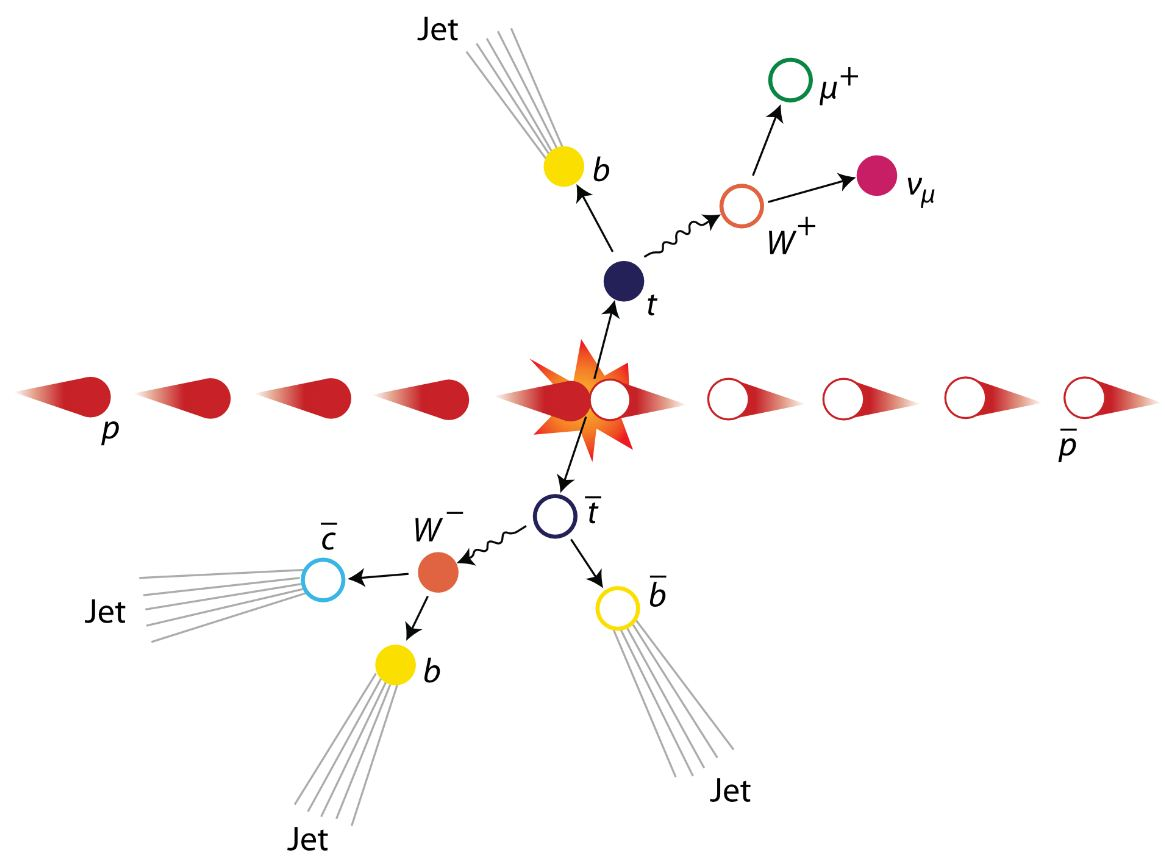
\includegraphics[width=10cm]{figure/collision.JPG}}
%{\centering 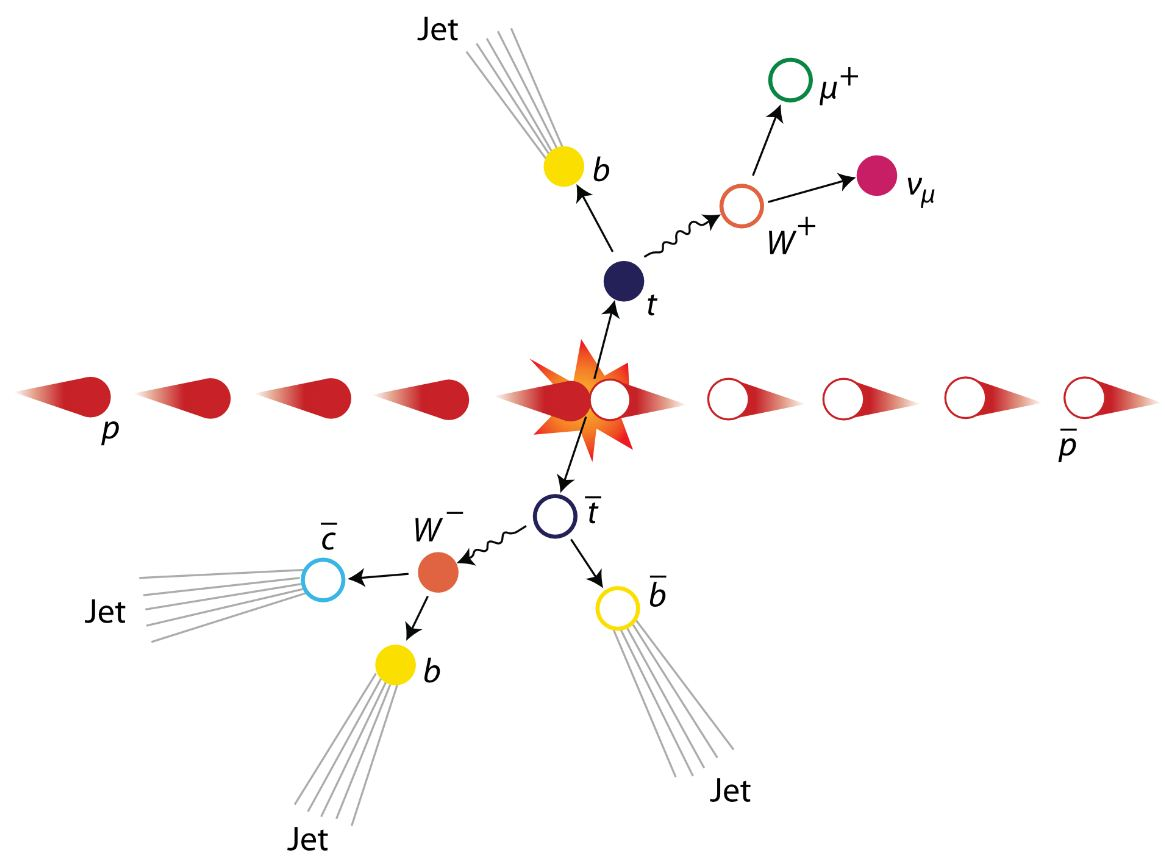
\includegraphics[width=10cm]{figure/collision.JPG}}
\caption[Colisi�n entre part�culas y part�culas secundarias producidas]{Colisi�n entre part�culas y part�culas secundarias producidas.\label{fig:collision}}
\end{figure}


El proceso de detecci�n no es un trabajo simple, primero se debe comprender que para cada tipo de part�culas y para cada variable a analizar existen distintos tipos de detectores con diferentes propiedades de detecci�n. Estos detectores a su vez pueden variar mucho entre ellos, bas�ndose en principios f�sicos muy distintos. Debido a que en los colisionadores las part�culas producidas pueden ser de una gran cantidad de tipos, en diferentes rangos de energ�as, un detector en un acelerador puede estar compuesto por diversos sub-detectores que deben trabajar en conjunto para obtener una imagen completa del evento. Adem�s de las complicaciones inherentes al proceso de detecci�n, se debe considerar toda la electr�nica asociada al trabajo de lectura de las se�ales. Esto involucra el tratamiento electr�nico de las se�ales, la digitalizaci�n, el procesamiento en computadoras, entre otros.

A�adido a todo esto se debe observar que los colisionadores pueden producir una cantidad gigantesca de datos, colisionadores como el LHC ubicado en Suiza produce alrededor de 600 millones de colisiones por segundo (en datos se producir�n 25 GB/s en la actual corrida del detector). Esto agrega la necesidad de que todo el proceso de detecci�n debe ser muy r�pido y eficiente, o en otras palabras, la detecci�n debe ser muy escalable.

Si bien el proceso de detecci�n entrega datos en bruto de las part�culas detectadas es necesario procesar estos datos computacionalmente con la finalidad de obtener informaci�n �til para ser utilizada en el an�lisis. De esto �ltimo se encarga el procedimiento conocido como reconstrucci�n. Durante este paso los datos en bruto entregados por el detector son procesados utilizando m�todos estad�sticos y modelos te�ricos en f�sica con la finalidad de inferir el proceso mediante el cual los datos finales fueron producidos, es decir identificar las part�culas que dieron origen a los datos observados y sus propiedades. Al igual que en los detectores, existe una gran cantidad de opciones para el proceso de reconstrucci�n, dependiendo del detector del que provienen los datos, el tipo de part�cula a ser identificada, el rango de energ�a en que se opera, etc�tera. 

A continuaci�n se proceder� a entregar una muy breve introducci�n a los diferentes tipos de detectores que son utilizados en la f�sica experimental, un an�lisis m�s t�cnicos del funcionamiento de estos ser� abordado en la Secci�n 2.

\subsection{Tipos de detectores}

Como una primera clasificaci�n los detectores pueden agruparse en dos grupos, detectores de part�culas cargadas y detectores de part�culas neutras. Mientras que la part�culas cargadas pueden ser detectadas directamente mediante diversos m�todos, la �nica forma de detectar part�culas neutras es hacerlas interactuar en el detector con la finalidad de que produzcan part�culas cargadas secundarias que puedan ser detectadas y luego reconstruir las part�culas neutras mediante la informaci�n de las part�culas secundarias. 

Los detectores de part�culas neutras se pueden clasificar seg�n la part�cula a detectar:
\begin{itemize}
\item Los detectores de fotones ($\gamma$) usan las interacciones electromagn�ticas de los fotones con la materia, es decir el efecto fotoel�ctrico, efecto compton y la creaci�n de pares. Aqu� son �tiles los detectores calor�metros que ser�n analizados m�s adelante.
\item La detecci�n de neutrinos ($\nu$)  utiliza la interacci�n d�bil de estos con la materia, debido a que esta es la �nica fuerza que los afecta. Dado que la probabilidad de interacci�n de los neutrinos es muy baja el proceso de detecci�n es considerablemente m�s complicado. 
\item Los detectores de neutrones ($n$) hacen uso de la interacci�n fuerte de estos con la materia. Un ejemplo es hacer uso de la colisi�n el�stica entre un proton y un neutr�n, en esta, el proton adquiere energ�a y se puede utilizar esto para detectar el neutr�n.
\end{itemize}

Los detectores de part�culas cargadas, por otro lado, pueden ser clasificados seg�n el proceso que utilizan para medir las propiedades de las part�culas con carga.
\begin{itemize}
\item Los detectores electr�nicos miden los electrones liberados por ionizaci�n. Estos electrones acelerados en un potencial producen a su vez m�s ionizaci�n generando una avalancha que produce una se�al medible. El medio de ionizaci�n puede ser un gas ( por ejemplo en los detectores Geiger-M�ller o en los contadores proporcionales) o puede ser un cristal semiconductor donde la avalancha es generada por la creaci�n de pares $e^-$-hueco.
\item En la detecci�n por trazas se utiliza un medio en el cual la trayectoria de la part�cula se hace visible (c�maras de niebla, de burbujas, de emulsiones, de chispas, entre otras). En presencia de un campo el�ctrico $\vec{B}$ las trayectoria de la part�culas es curvada en funci�n de su momento, lo que permite estimarlo.
\item Los contadores por centelleo y de Cherenkov detectan la emisi�n luminosa de las part�culas que son excitadas por las part�culas incidentes. Estos fotones pueden ser medidos utilizando el efecto fotoel�ctrico y amplificadores del pulso el�ctrico (fotomultiplicadores).
\end{itemize}
De especial inter�s en este trabajo son los detectores Calor�metros, que se proceder�n a describir a continuaci�n.
\subsection{Detector Calor�metro}
Los detectores del tipo calor�metros son muy �tiles para medir la energ�a total de una o m�s part�culas (tanto neutras como cargadas). Pueden ser de dos tipos: calor�metros electromagn�ticos o calor�metros hadr�nicos. Los calor�metros electromagn�ticos son capaces de medir la energ�a de las part�culas incidentes mediante la producci�n de lluvias electromagn�ticas, compuestas de $e^{\pm}$ y $\gamma$ mediante procesos de creaci�n de pares y radiaci�n de frenado (a altas energ�as)~\cite{davies1954theory}. Los calor�metros hadr�nicos, en cambio, miden la energ�a de la part�cula mediante la generaci�n de lluvias hadr�nicas mediante interacciones del tipo fuerte. Ambos pueden ser homog�neos o heterog�neos (o de muestreo). Un calor�metro de muestreo intercala  capas de materiales sensibles y materiales de producci�n de las lluvia (un ejemplo de este tipo de calor�metros es el \emph{Hadron Calorimeter (HCAL)} del experimento CMS en CERN). El calor�metro homog�neo, por otro lado, esta compuesto en su totalidad por materiales sensibles. Estos materiales sensibles pueden ser cristales centelleadores (BGO, LYSO), cristales de vidrio de plomo, arg�n liquido, entre otros. 

Este trabajo en particular tratar� con un calor�metro de tipo electromagn�tico, por lo que se ahondar� m�s en este tipo de calor�metros en la pr�xima secci�n.

\subsection{Magnitudes de los detectores}
Diferentes tipos de detector sirven para medir distintas part�culas, estos, a su vez se pueden diferenciar en sus materiales de construcci�n, la disposici�n de estos materiales, su tama�o, etc�tera. Para evaluar la eficacia de un detector hay varias variables a considerar:
\begin{itemize}
\item \textbf{Resoluci�n energ�tica:} Mide la capacidad del detector para medir con exactitud la energ�a de la part�cula incidente, esta se define como $ R =\Delta E/E_0 $, donde $\Delta E$ es el ancho en la altura media de una normal ajustada a la se�al medida y $E_0$ es el valor de la part�cula incidente.
\item \textbf{Resoluci�n espacial:} Esta variable mide la capacidad de identificar espacialmente part�culas cercanas entre s�. Se puede entregar en forma de desviaci�n est�ndar $\sigma_x$.
\item \textbf{Sensibilidad:} Mide la capacidad del detector para producir una se�al de salida medible �til, dada una entrada. Mayor sensibilidad corresponde a un detector capaz de detectar mayor parte de la energ�a de una part�cula incidente. Detectores peque�os tendr�n una baja sensibilidad y s�lo detectaran parte de la energ�a de la part�cula.
\item \textbf{Eficiencia:}  Com�nmente un detector no es capaz de responder al paso de todas las part�culas que lo atraviesan. La eficiencia $\xi$ corresponde a la raz�n \emph{n�mero de part�culas detectadas / n�mero de part�culas incidentes}. 
Esta puede ser descompuesta en una eficiencia gemetrica $\xi_{geo}$ que es consecuencia del tama�o del detector y su distancia a la fuente de part�culas y una eficiencia intr�nseca $\xi_{int}$ que se relaciona con la probabilidad de interacci�n del material del detector. 
\item \textbf{Tiempo muerto:} Esta variable mide el tiempo de inoperabilidad entre la detecci�n de part�culas. Pone un l�mite inferior a la capacidad del detector para contar part�culas muy cercanas temporalmente. 
\end{itemize} 

En un calor�metro electromagn�tico la resoluci�n espacial es un factor clave a considerar. El problema de identificar part�culas muy cercanas entre s� es universal en la f�sica de altas energ�as (o HEP, por las siglas de \emph{High Energy Physics}) y es de inter�s particular en los coleccionadores Electr�n-I�n debido a la alta proporci�n de fotones, electrones y positrones en la colisi�n. Un caso muy com�n en que se presenta este problema es en el decaimiento de un pion neutro en dos fotones muy cercanos entre s�. Si la resoluci�n no es suficiente es muy dif�cil identificar dos fotones generados por este tipo de decaimiento de un s�lo fot�n de alta energ�a. 

Como ejemplo concreto, el detector ECAL (por \emph{Electromagnetic Calorimeter}) del colisionador CMS en CERN tiene como prop�sito identificar el decaimiento del boson de Higgs en dos fotones. Para hacer esto es necesario identificar los diferentes eventos background que se comportan similar, pero no corresponden al boson de Higgs. Uno de estos eventos es el decaimiento de un pion neutro en dos fotones cercanos entre s�. El detector ECAL esta conformado por una matriz de cristales del tipo $PbWO_4$ (tungsteno de plomo) como se muestra en la Figura~\ref{fig:ecal}, el tama�o transversal de cada cristal define la resoluci�n espacial del detector. Hacia los extremos del detector el �ngulo entre los fotones producidos por el decaimiento de un pion neutro es mucho menor y la resoluci�n espacial del detector ECAL no es suficiente, como se muestra mediante simulaciones en la Figura ~\ref{fig:pion0_ecal}. Con la finalidad de solucionar este problema se utiliza un detector de alta resoluci�n y sensible a los fotones incidentes que se coloca delante del detector calor�metro, conocido como detector preshower. El detector preshower es capaz de distinguir fotones muy cercanos entre s� y de esta manera rechazar eventos background provenientes del decaimiento del pion neutro.  El detector preshower de CMS esta compuesto por capas de plomo, que producen las lluvias electromagn�ticas y capas sensibles de silicio.

 \begin{figure}[t]
\makebox[\textwidth][c]{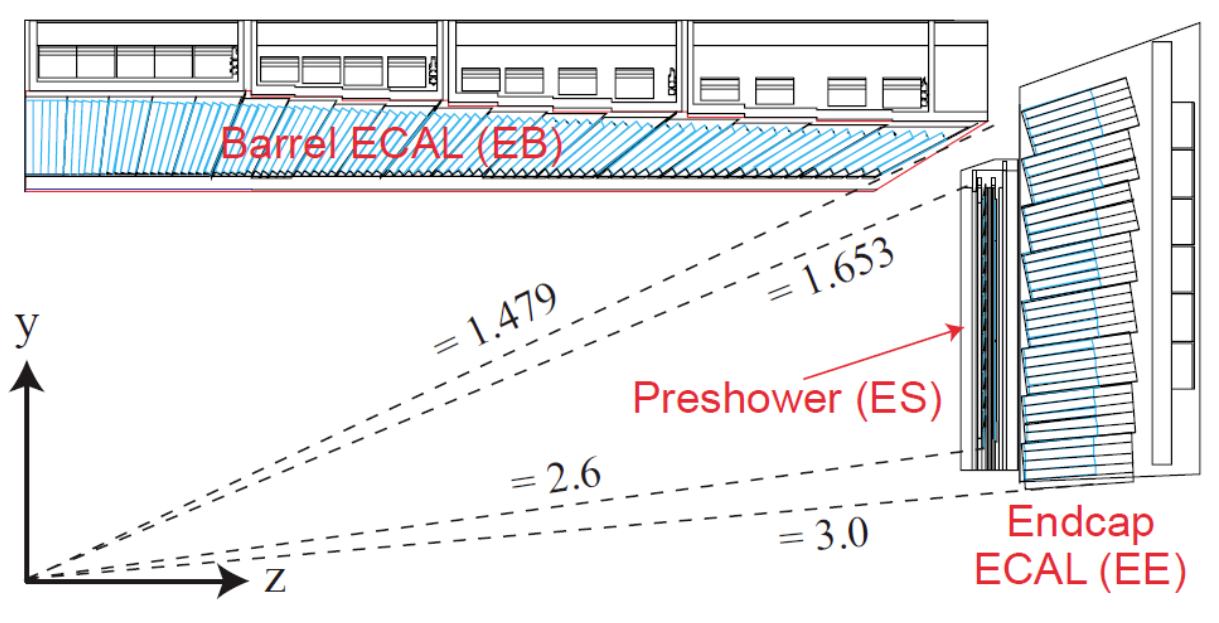
\includegraphics[width=10cm]{figure/ecal_design.png}}
%{\centering 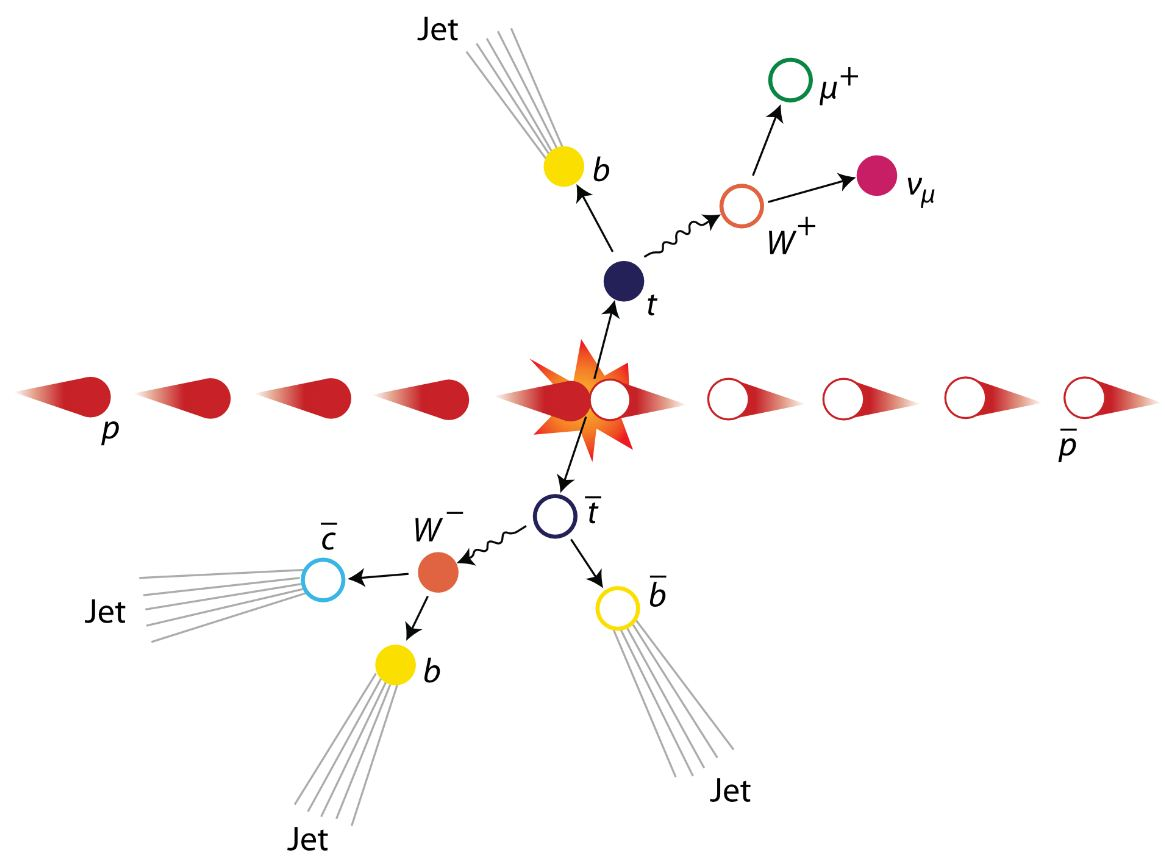
\includegraphics[width=10cm]{figure/collision.JPG}}
\caption{Dise�o de detector ECAL en CMS.\label{fig:ecal}}
\end{figure}
\begin{figure}[t]
    \centering
    \begin{subfigure}[b]{0.3\textwidth}
        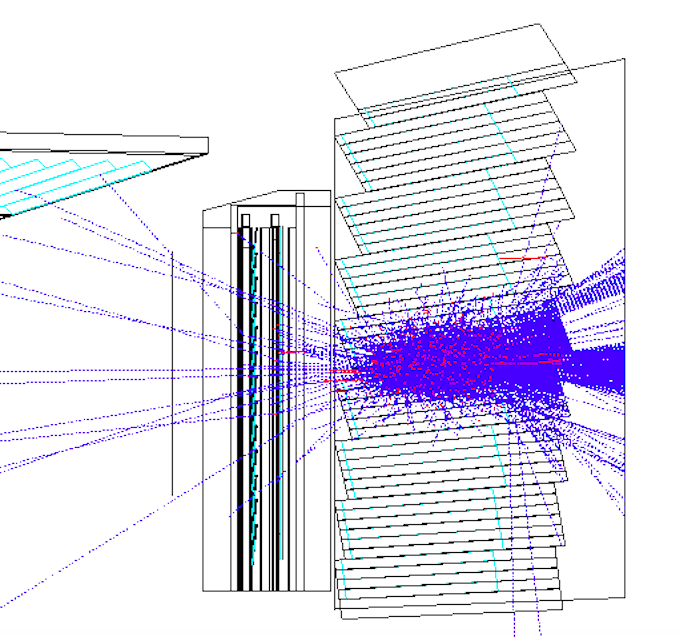
\includegraphics[clip, trim=0.5cm 0.5cm 0.5cm 0.5cm, width=\textwidth]{figure/gamma_2.png}
        \caption{Un foton siendo detectado por ECAL.}
        \label{fig:gamma2_ecal}
    \end{subfigure}
    ~
    \begin{subfigure}[b]{0.3\textwidth}
        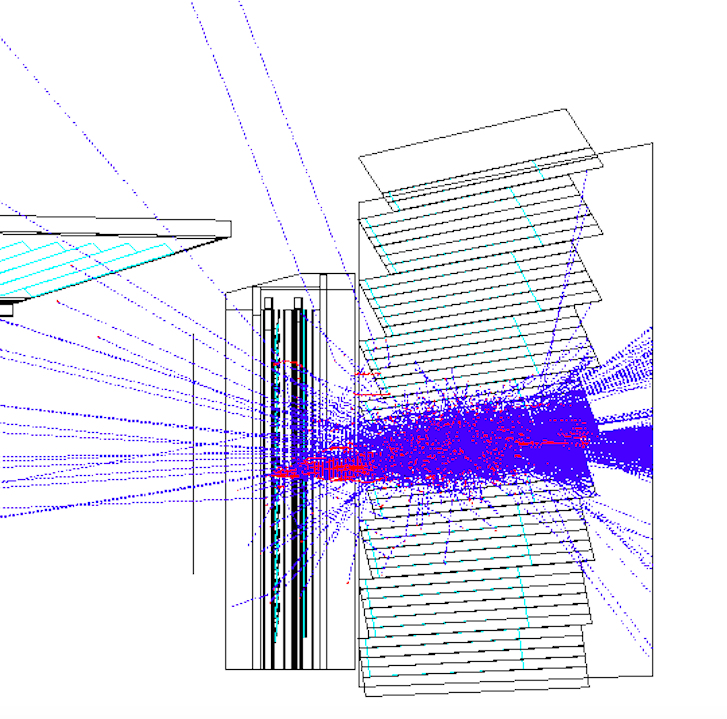
\includegraphics[clip, trim=0.5cm 0.5cm 0.5cm 0.5cm,width=\textwidth]{figure/pi0_2.png}
        \caption{Decaimiento de un pion neutro detectado por ECAL.}
        \label{fig:pion0_ecal}
    \end{subfigure}
\end{figure}

\section{Contexto}
Como ya se mencion�, el problema de identificaci�n de piones neutrales es de part�cular inter�s para cualquier colisionador Electri�n-I�n. En este contexto, los laboratorio BNL (\emph{Brookhaven National Laboratory}) y JLab (\emph{Thomas Jefferson Laboratory}), en conjunto con la oficina de f�sica nuclear del departamento de energ�a de Estados Unidos convocaron propuestas en torno a un programa R\&D en busca de satisfacer los requerimientos de un futuro colisionador EIC (\emph{Electron-Ion Collider}). En torno a esta convocatoria, la propuesta por parte de investigadores del Centro Cient�fico y Tecnol�gico de Valpara�so (CCTVal)~\cite{will_kuleshov} para construir un detector preshower para calor�metros fue aceptada. El detector podr�a ser utilizado en experimentos como CMS en CERN o IC de CLAS en Jefferson Lab.

Si bien existen calor�metros preshower basados en materiales como silicio, plomo o tungsteno, lo innovador de la propuesta del CCTVal es la exploraci�n de un calor�metro preshower basado en una matriz de cristales, lo que permite estudiar una alternativa con costos y caracter�sticas muy diferentes a la tecnolog�a actualmente en uso. Los detectores basados en cristales se han desarrollado con gran �xito en campos como la medicina nuclear, para la visualizaci�n mediante radiaci�n de tejidos internos (usando tom�grafos de emisi�n de positrones, PET). Cristales destelladores del tipo LYSO (Lutetium Yttrium Silicon Oxide) han logrado un gran protagonismo debido a que ofrecen cualidades de producci�n de lluvia excepcionales, adem�s que la industria de producci�n industrial de estos cristales esta bien desarrollada. Estas ventajas hacen que la exploraci�n de un dise�o basado en cristales para la detecci�n de alta resoluci�n espacial sea muy interesante. El detector preshower debe cumplir varias exigencias: 
\begin{itemize}
\item La capacidad de identificar dos part�culas muy cercanas entre s� depender� del tama�o transversal de cada cristal y de la secci�n longitudinal de estos. Ambos factores pueden ser optimizados para lograr una resoluci�n que permita identificar la mayor�a de los eventos problem�ticos. Si la distancia entre dos fotones es menor que la mitad del tama�o transversal de cada cristal, ser� muy dif�cil identificar ambos fotones correctamente, por lo que es recomendable utilizar cristales de tama�o transversal menor.
\item La superficie no sensitiva del detector preshower debe ser minimizada, con la finalidad de evitar la perdida de energ�a debido a interacci�n con materiales de lectura u otros instrumentos. Para esto se propone la utilizaci�n de un sistema especial de lectura ubicado en el frente del detector. 
\end{itemize}

La contribuci�n principal de este trabajo es la propuesta e implementaci�n de un algoritmo de reconstrucci�n completo para el detector preshower. Debido al dise�o innovador del detector, muchos de los componentes del algoritmo de reconstrucci�n son una contribuci�n nueva, mientras que otros componentes deben ser adaptados de la literatura para ser utilizados en conjunto con la singular composici�n del detector preshower. 

En lo que continua del trabajo se proceder� a describir de manera general la composici�n y funcionamiento del detector preshower, para luego continuar con la presentaci�n del algoritmo de reconstrucci�n y finalmente estudiar la efectividad del algoritmo mediante experimentos en datos simulados y reales. En la Secci�n 2 se introducir�n algunos conceptos fundamentales en f�sica de detectores, vitales para comprender de manera general el funcionamiento del detector preshower. Luego, en la Secci�n 3, se explicar� de manera general la composici�n y funcionamiento del detector preshower. En la Secci�n 4 se analizar�n las diferentes alternativas presentes en la literatura para la reconstrucci�n de part�culas en calor�metros. Se continuar� en la Secci�n 5 con la presentaci�n del algoritmo de reconstrucci�n propuesto. En la Secci�n 6, experimentos en datos simulados y datos reales para estudiar la capacidad del algoritmo de reconstrucci�n ser�n expuestos para finalmente, en la Secci�n 7, concluir sobre estos resultados.



    \chapter{Detectores de part�culas \label{conceptos-fisica}}
En esta secci�n se analizar�n los conceptos f�sicos relacionados a la detecci�n en calor�metros. Para un tratamiento de los conceptos f�sicos b�sicos relacionados a la interacci�n general de part�culas con la materia el lector se puede dirigir al Ap�ndice A.

\section{F�sica de los detectores calor�metros}
Si bien la f�sica involucrada en el funcionamiento de los detectores es amplia y variada aqu� nos concentraremos en los detectores del tipo calor�metro, que son el eje principal de este trabajo. En lo que sigue de esta secci�n se realizar� una descripci�n de los procesos que ocurren en un detector calor�metro de manera general con la finalidad de entregar una base te�rica para comprender las desiciones de dise�o en la construcci�n del detector preshower. Tambi�n, como ya se mencion�, un calor�metro puede ser del tipo homog�neo o heterog�neo (o de muestreo) seg�n la disposici�n de sus partes o, adem�s, del tipo electromagn�tico o hadr�nicos seg�n el tipo de part�cula que detecten. Aqu� nos concentraremos en los elementos constitutivos de un calor�metro del tipo electromagn�tico y su funcionamiento. 

Un calor�metro se conforma de un material de producci�n de lluvias electromagn�ticas y un material de lectura de estas lluvias. Para comprender mejor esto a continuaci�n se describir�n los procesos que originan las lluvias electromagn�ticas.
\subsection{Lluvias electromagn�ticas}\label{sec:lluvias}
La generaci�n de lluvias electromagn�ticas es un proceso producido por el efecto combinado de la producci�n de pares y la emisi�n por radiaci�n de frenado (o bremsstahlung). A altas energ�as un fot�n se convierte en un par $e^+e^-$, estos a su vez emiten fotones mediante el proceso de radiaci�n de frenado, estos fotones producen pares $e^+e^-$ y el proceso continua intercalando ambos procesos como se muestra en la Figura \ref{fig:shower}, hasta alcanzar la energ�a cr�tica. El proceso es descrito de manera aproximada por el modelo de Heitler.

\begin{figure}[t]
\makebox[\textwidth][c]{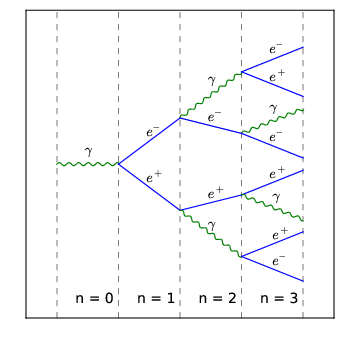
\includegraphics[width=8cm]{figure/em_shower.png}}
%{\centering 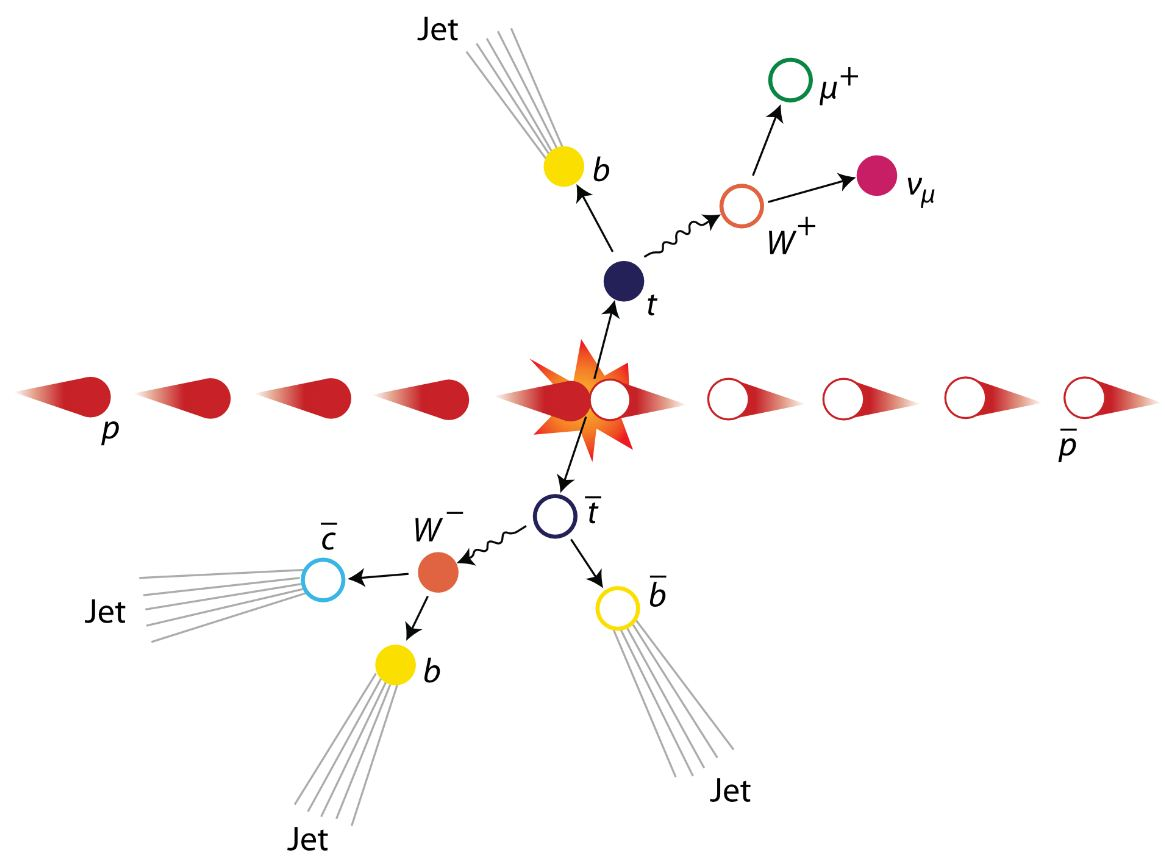
\includegraphics[width=10cm]{figure/collision.JPG}}
\caption[Colisi�n entre part�culas y part�culas secundarias producidas]{Diagrama de una lluvia electromagn�tica, descrita por el modelo Hetiler.\label{fig:shower}}
\end{figure}

En el modelo de Heitler, en promedio un fot�n se convertir� en un par electr�n-positron en una longitud de radiaci�n $X_0$. Entonces un fot�n de $E_0$ que entra en el calor�metro producir� alrededor de $2^t$ part�culas al cabo de $t$ longitudes de radiaci�n. Es decir,
\begin{equation}
N(t) = 2^t. \nonumber
\end{equation}
Adem�s, dado a que en cada paso la energ�a de cada par ser� un medio de la part�cula que lo produce, entonces 
\begin{equation}
E(t) = \frac{E_0}{2^t}, \nonumber
\end{equation}
o, trabajando esta ecuaci�n, la energ�a media de las part�culas a la profundidad $t$ ser�,
\begin{equation}
t(E') = \frac{\ln(E_0/E')}{\ln2}. \nonumber
\end{equation}
Como ya se mencion�, la lluvia se detiene al alcanzar la energ�a cr�tica $E_c$, en la que los pares $e^+e^-$ empiezan a perder su energ�a por colisiones at�micas en vez que por radiaci�n de frenado. Asumiendo que la cascada (o lluvia) se detiene abruptamente a esta energ�a tenemos que el m�ximo n�mero de part�culas se alcanza a  
\begin{equation}
t_{max} = \frac{\ln(E_0/E_c)}{\ln 2}, \nonumber
\end{equation}
donde el n�mero de part�culas es,
\begin{equation}
N_{max} = e^{t_{max}\ln2} = E_0/E_c, \nonumber
\end{equation}
y la suma de recorrido de las part�culas es,
\begin{equation}
L = X_0 \int^{t_{max}}_0 N(t) dt \approx X_0\frac{E_0/E_c}{\ln2}. \nonumber
\end{equation}
Es decir, midiendo $N_{max}$, $L$ o una cantidad proporcional es posible conocer el valor de energ�a inicial de la part�cula incidente. Se debe notar eso si, que el modelo es solo una aproximaci�n simple de la lluvia, es posible obtener aproximaciones m�s cercanas mediante m�todos de Monte Carlo (es imposible obtener una forma anal�tica).

El desarrollo longitudinal de la lluvia se puede cuantificar utilizando el radio de Moliere. A la profundidad m�xima, el valor medio del �ngulo de apertura de las part�culas puede ser aproximado como
\begin{equation}
<\theta> = \frac{21.2 MeV}{E_c}, \nonumber
\end{equation} 
entonces, el radio de Moliere se define como	
\begin{align}
\rho_M &= <\theta>X_0 \nonumber\\
&=  \frac{21.2 MeV}{E_c} X_0 \nonumber\\
&= 7(g/cm^2)\frac{A}{Z},\nonumber
\end{align} 
que puede ser comprendido como la distancia transversal que una part�cula en la energ�a cr�tica viaja al atravesar una longitud de radiaci�n. Adem�s, 
el $90\%$ de la energ�a de la lluvia esta contenida en alrededor de un $\rho_M$. En al Figura \ref{fig:Moliere} se muestra como la distribuci�n de la energ�a transversal integrada en la direcci�n longitudinal se desarrolla como funci�n de la direcci�n en radios de Moliere desde la posici�n incidente de la part�cula. 
\begin{figure}[t]
\makebox[\textwidth][c]{\includegraphics[width=8cm]{figure/Moliere.png}}
%{\centering 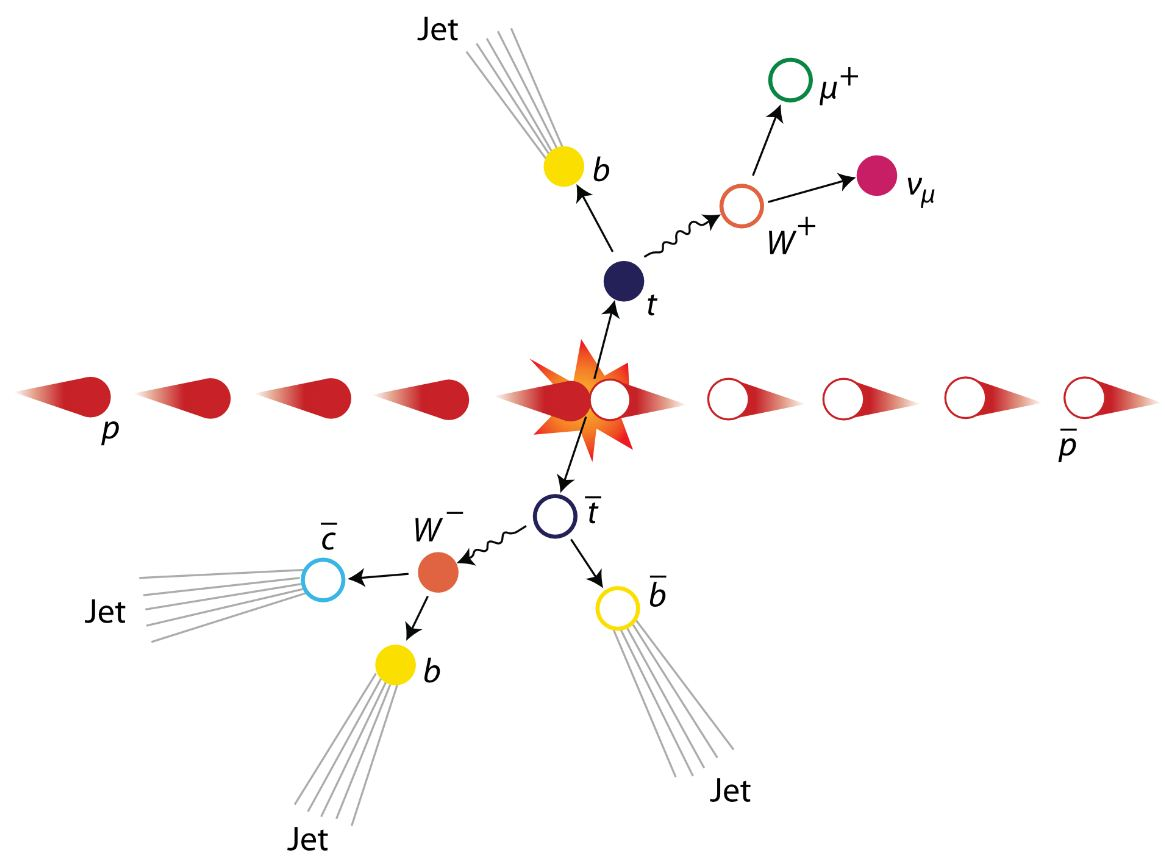
\includegraphics[width=10cm]{figure/collision.JPG}}
\caption{Desarrollo tranversal de la cascada electromagn�tica en funci�n del n�mero de radios de Moliere desde la posici�n incidente, para distintos materiales.\label{fig:Moliere}}
\end{figure}
Esta cantidad es muy importante en el dise�o del calor�metro cuando la resoluci�n espacial es un factor clave a considerar. Un menor radio de Moliere significa una mejor resoluci�n espacial y por lo tanto una mejor capacidad para separar cascadas solapadas.
\subsection{Materiales de construcci�n}
Si bien, como ya se mencion�, un calor�metro electromagn�tico puede estar construido de diferentes tipos de materiales (l�quidos y s�lidos, org�nicos e inorg�nicos), en este trabajo nos concentraremos en la construcci�n de calor�metros homog�neos con cristales centelleadores inorg�nicos (BGO, LYSO, LSO). Dos son los principales componentes de este tipo de calor�metros, el material centelleador y el sistema de lectura, que se proceder�n a describir a continuaci�n.
\subsection{Cristales centelleadores}
Los cristales centelleadores son al mismo tiempo materiales activos (generadores de lluvias electromagn�ticas) y sensibles (mediante la generaci�n de luz por centelleo). Estos son capaces de generar luminiscencia al desexcitarse los �tomos que son excitados por el paso de part�culas cargadas. En espec�fico, la captura de electrones por impurezas (o centros de activaci�n) del cristal produce emisi�n de luz al desexcitarse. Existen dos tipos de emisi�n, la fluorescencia, de tipo muy r�pido ($\tau \sim 10^{-8} seg.$) y la fosforescencia, que es muy lenta ($\tau_d \sim \mu s$). Para los detectores se prefieren materiales con tiempos de desexcitaci�n muy r�pidos. La respuesta del centelleador es lineal a la energ�a depositada y se busca una alta eficiencia, r�pida respuesta, con transparencia a la radiaci�n fluorescente y un espectro de emisi�n similar al de los fotomultiplicadores utilizados en la lectura. Un valor importante para medir la calidad de un centelleador es su respuesta luminosa. Esta se define como la energ�a necesaria para crear un fot�n de centelleo, o 
\begin{equation}
\eta = \frac{\Delta E}{N_\gamma}. \nonumber
\end{equation} 
Este valor se puede entender como la eficiencia del detector para producir una se�al medible.
Esta eficiencia tambi�n es afectada por distintos procesos en el transporte de la luz, por ejemplo existe una atenuaci�n en la propia luz de centelleo seg�n la ley de atenuaci�n $N(x) = N_0 e^{-\mu x}$ con $\mu$ el coeficiente de atenuaci�n. 

Los fotones producidos por el centelleador son com�nmente traspasados al fotomultiplicador que convierte los pulsos de luz en corriente el�ctrica. La luz es trasladada al fotomultiplicador por gu�as de luz que pueden, a su vez, cambiar el rango de frecuencia de la luz emitida por el centelleador. Un diagrama se muestra en la Figura \ref{fig:centelleador}.

\begin{figure}[t]
\makebox[\textwidth][c]{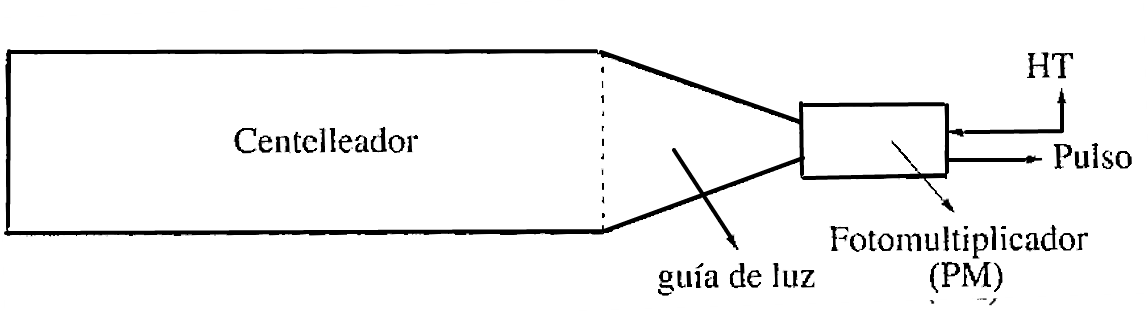
\includegraphics[width=12cm]{figure/centelleador.png}}
%{\centering 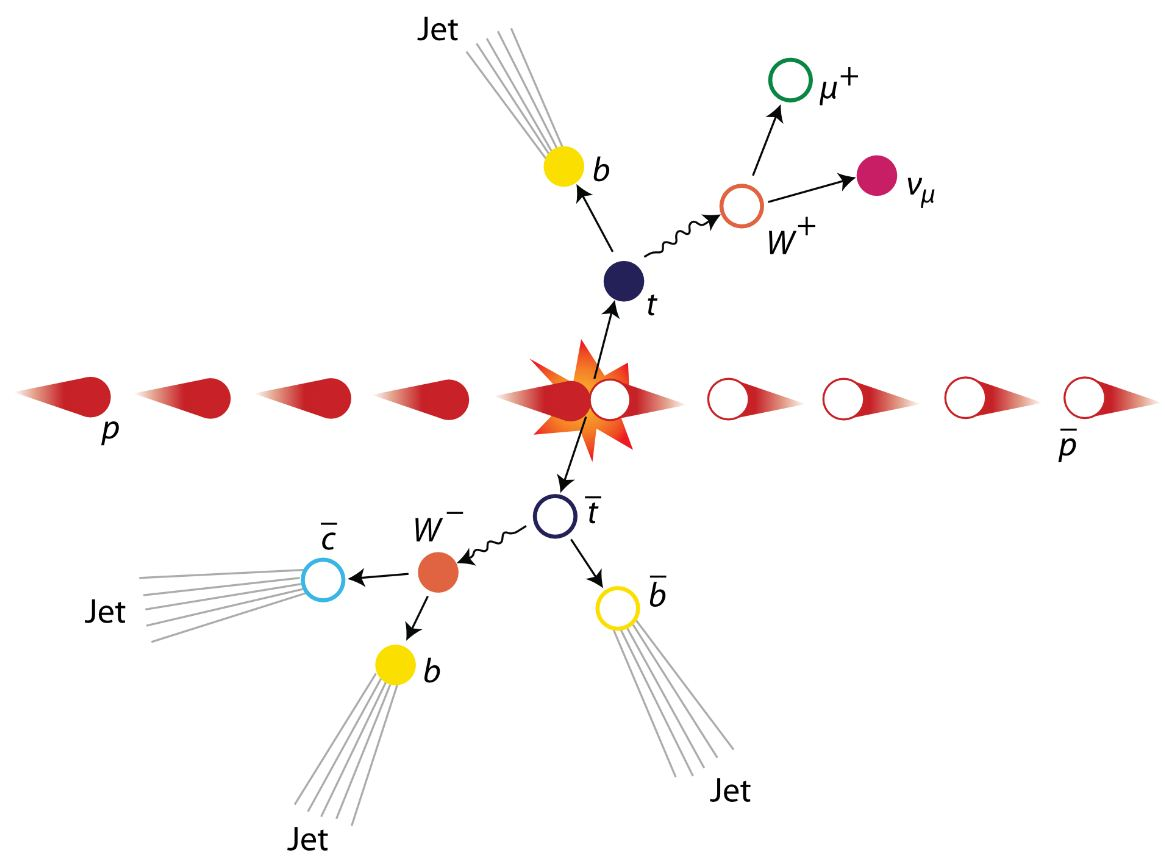
\includegraphics[width=10cm]{figure/collision.JPG}}
\caption{Diagrama simple de un centelleador conectado a un fotomultiplicador.\label{fig:centelleador}}
\end{figure}

\subsection{Fotomultiplicadores} \label{sec:fotomultiplicadores}
Los fotomultiplicadores son capaces de convertir pulsos de luz en pulsos de corriente el�ctrica medibles. Se componen del fotoc�todo, d�nodo y �nodo.
El fotoc�todo emite electrones en respuesta a los fotones incidentes mediante efecto fotoel�ctrico. El material que lo compone debe ser un semiconductor con gran probabilidad de efecto fotoel�ctrico. Com�nmente, los electrones producidos por el efecto fotoel�ctrico se refieren como fotoelectrones $\gamma_e$. La eficiencia cu�ntica se puede definir como 
\begin{equation}
\eta(\lambda) = \frac{N_{\gamma_e}}{N_{\gamma_{inc}}}, \nonumber
\end{equation} 
donde $ N_{\gamma_e}$ y $N_{\gamma_{inc}}$ es el n�mero de fotoelectrones producidos y el n�mero de fotones incidentes respectivamente. Adem�s, $\lambda$ es la longitud de onda de los fotones incidentes.

Los d�nodos son los encargados de multiplicar los fotoelectrones producidos en el c�todo. En estos, los fotoelectrones son acelerados en presencia de un campo el�ctrico y dirigidos a los d�nodos, dispuestos seg�n la Figura \ref{fig:fotomultiplicador}, los que a su vez producen la emisi�n secundar�a de m�s electrones. 

El �nodo recoge la avalancha final de electrones producidos por los d�nodos y produce un pulso el�ctrico, normalmente un voltaje en funci�n del tiempo $V(t)$.  La ganancia del fotomultiplicador se puede definir como la amplificaci�n en la cadena de d�nodos. Si cada d�nodo produce $\delta$ electrones secundarios, entonces la ganancia ser�
\begin{equation}
G = \delta^n = (KV_d)^n, \nonumber
\end{equation} 
donde $V_d$ es el potencial entre d�nodos y $n$ el n�mero de d�nodos. Se debe notar adem�s que debido a que el funcionamiento de los centelleadores suele ser muy r�pido, el fotomultiplicador tambi�n debe tener una resoluci�n temporal muy alta.
\begin{figure}[t]
\makebox[\textwidth][c]{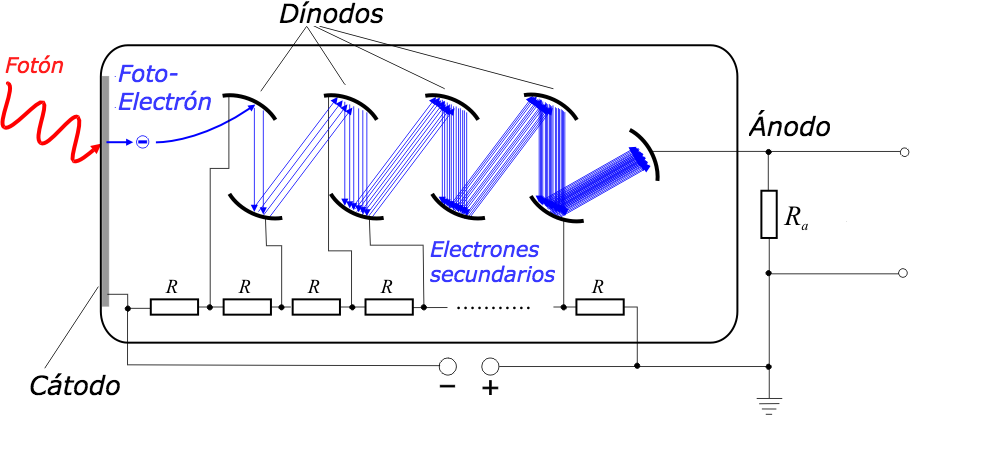
\includegraphics[width=15cm]{figure/fotomultiplicador.png}}
%{\centering 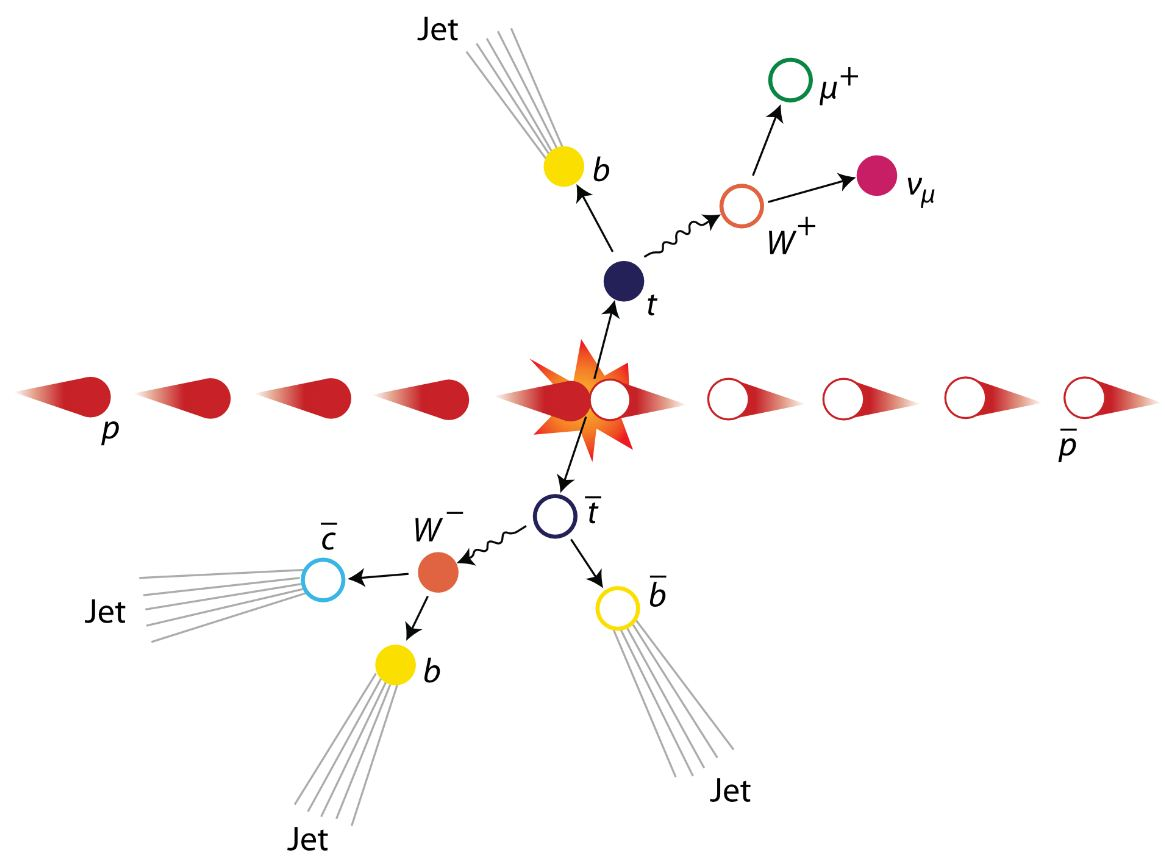
\includegraphics[width=10cm]{figure/collision.JPG}}
\caption{Fotomultiplicador en funcionamiento.\label{fig:fotomultiplicador}}
\end{figure}

Habiendo realizado un resumen muy general de los conceptos principales a tener en cuenta en el dise�o de un calor�metro, en la pr�xima secci�n presentaremos el calor�metro preshower, su estructura general y las bases de su funcionamiento. La secci�n siguiente constituir� una visi�n general del dise�o del preshower, s�lo lo necesario para comprender a cabalidad el algoritmo de reconstrucci�n propuesto para el detector preshower.


    \chapter{Detector Preshower \label{detector}}
En esta Secci�n se proceder� a describir, de manera general, el dise�o y funcionamiento del detector preshower. Como ya se mencion�, la finalidad del detector preshower es detectar part�culas (neutras y cargadas) muy cercanas entre s�, por lo que el dise�o esta pensado en pos de esta finalidad. Un primer acercamiento por parte del equipo experimental de f�sica nuclear y de altas energ�as de la UTFSM corresponde a un prototipo simple para probar el funcionamiento del detector antes de entrar en una fase de producci�n.
Primero, se presentar� el dise�o general del prototipo para luego explicar las bases de su funcionamiento.

\section{Dise�o}
El detector preshower es un detector calor�metro electromagn�tico del tipo homog�neo. Como se describi� en la Secci�n 2, un detector calor�metro se conforma principalmente de un material de producci�n de lluvias (pueden ser cristales org�nicos e inorg�nicos, l�quido, gas, etc�tera) y un sistema de amplificaci�n y lectura de las se�ales producidas (por ejemplo un sistema de fotomultiplicadores).
En el prototipo de preshower estas dos secciones principales son la matriz de cristales que producen las lluvias electromagn�ticas y el sistema de lectura que convierte esta lluvia en una se�al medible. Un esquema a alto nivel del dise�o del detector se observa en le Figura~\ref{fig:preshower}.

\begin{figure}[t]
\makebox[\textwidth][c]{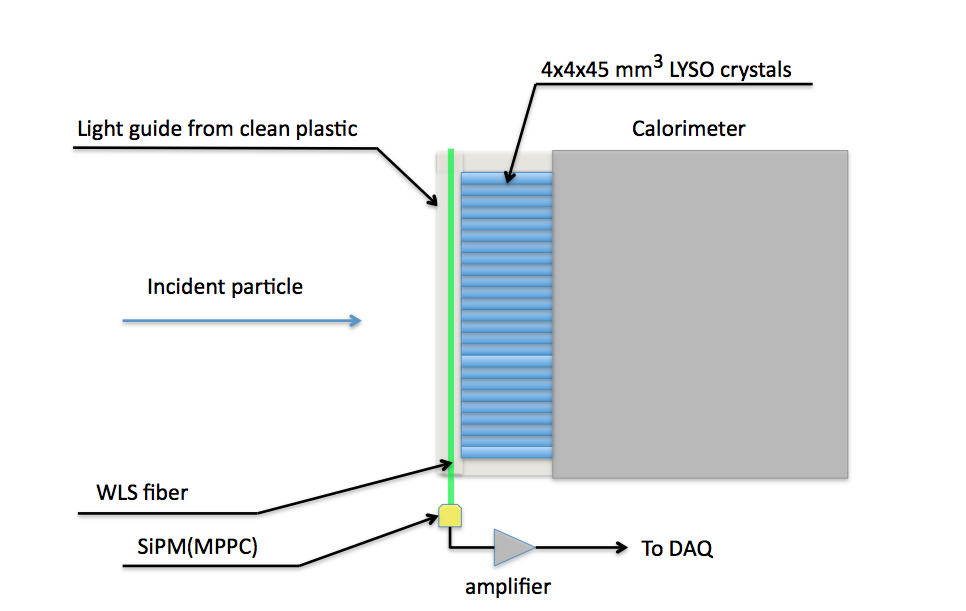
\includegraphics[width=15cm]{figure/preshower_proto_2.png}}
%{\centering 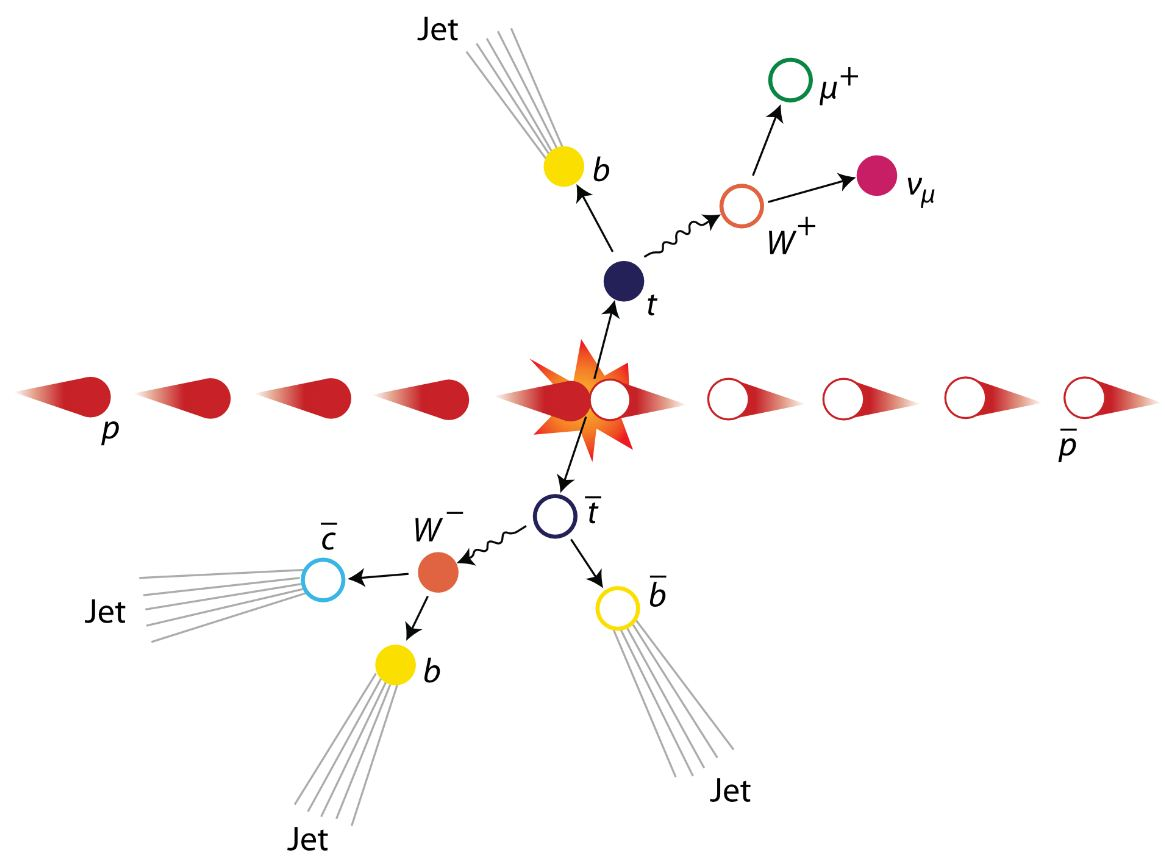
\includegraphics[width=10cm]{figure/collision.JPG}}
\caption{Prototipo de preshower, en este se pude observar la matriz de cristales (de color azul), el sistema de lectura y el material de cobertura.\label{fig:preshower}}
\end{figure}


\subsection{Matriz de cristales}
La matriz de cristales se conforma de 25x25 (625 en total) cristales centelleadores del tipo LYSO ($Lu_{1.8}Y_{0.2}SiO_5$). Como fue descrito en la Secci�n previa, los materiales centelleadores son capaces de producir luz mediante el proceso de luminiscencia, cuando part�culas cargadas interact�an con el material. Los cristales LYSO ofrecen ciertas caracter�sticas que lo hacen una muy buena elecci�n para la construcci�n del preshower, estos presentan un tipo de luminiscencia muy veloz e intensa, lo que permite reducir los tama�os del calor�metro y al mismo tiempo producir una se�al medible por el sistema de lectura. Otros materiales com�nmente utilizados como cristales centelleadores son BGO ($Bi_4 Ge_3 O_{12}$) y PWO ($PbWO_4$). Valores caracter�sticos de cada uno de estos materiales se muestran en la Tabla \ref{table:materiales}, que muestra claramente la superioridad en luminosidad (fotones producidos por energ�a incidente) de los cristales LYSO sobre las otras opciones. 

Otro valor importante a considerar es la longitud de atenuaci�n del cristal. Si bien el fabricante del cristal reporta un valor de $\lambda$ de $12[mm]$, otros estudios reportan valores muchos mayores [ESTUDIOS]. Recordar que la longitud de atenuaci�n se relaciona con la probabilidad de absorber o no una part�cula en el material, por lo que mayores longitudes de radiaci�n implicar�n cristales de mayor tama�o con la finalidad de aumentar la probabilidad de interacci�n con los cristales (de otra forma las part�culas pueden pasar sin interactuar y por lo tanto sin ser detectadas). Las probabilidades de interacci�n de una part�cula gamma entregadas por el fabricante, dependiendo de la energ�a y para varios largos del cristal, se muestran en la Figura \ref{fig:absorcion}. Para un largo de $45[mm]$ y un fot�n de $511[keV]$ la probabilidad de absorci�n es aproximadamente $95\%$, bajando a un largo de $4[mm]$ la probabilidad disminuye a un valor cercano a $4\%$. Esto demuestra la importancia de conocer correctamente la longitud de atenuaci�n con la finalidad de seleccionar correctamente el tama�o del cristal usado. Experimentos por parte del grupo de f�sica experimental del centro CCTVAL han medido una longitud de atenuaci�n de $1043\pm61[mm]$ mediante experimentos que miden el cambio en la posici�n del peak de energ�a medido por el lector (MPPC) dada la distancia de la part�cula incidente a este [TESIS ESTEBAN]. 

\begin{figure}[t]
\makebox[\textwidth][c]{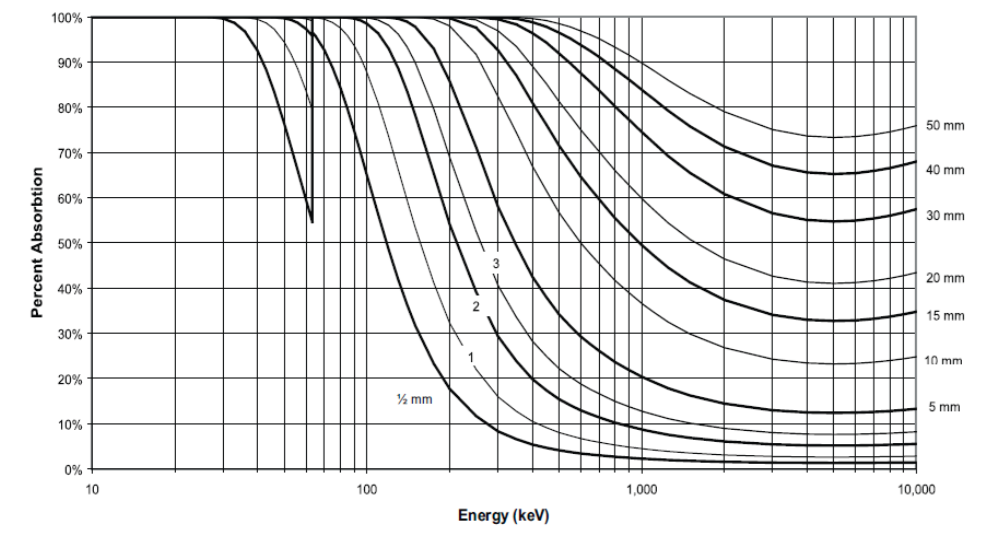
\includegraphics[width=15cm]{figure/absortion_lyso.png}}
%{\centering 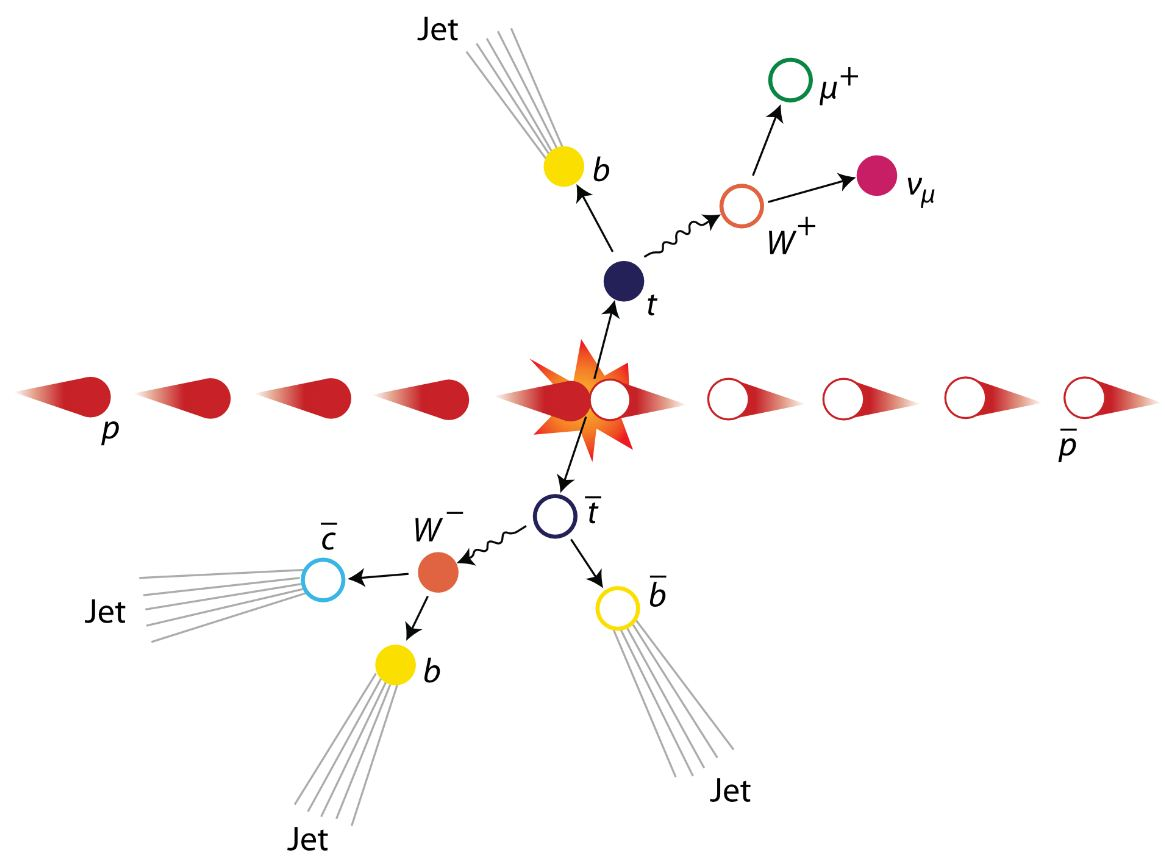
\includegraphics[width=10cm]{figure/collision.JPG}}
\caption{Porcentaje de absorci�n dada la energ�a para diversos largos de cristal LYSO. \label{fig:absorcion}}
\end{figure}


Finalmente, se utilizan cristales de tama�o 4x4x45 [mm$^3$], lo que (seg�n las especificaciones del fabricante) supone un dise�o de 4 longitudes de absorci�n. 

Es importante aislar �pticamente los cristales para evitar la salida de luz de cada cristal. La luz viaja en el cristal confinada por el material reflectante hasta alcanzar los extremos del cristal donde es absorbida y re-emitida por fibras �pticas. Adem�s, experimentos han demostrado que es posible optimizar la longitud de atenuaci�n con diferentes materiales reflectantes [EXPERIMENTOS WILL]. Los experimentos realizados para seleccionar el material reflectante se pueden encontrar en [TESIS ESTEBAN].

\subsection{Sistema de lectura}



    \chapter{Algoritmo de Reconstrucci�n \label{algoritmo}}

El algoritmo de reconstrucci�n es la propuesta principal de este trabajo, por lo que en esta secci�n se analizar� a fondo de que se trata un algoritmo de reconstrucci�n. Para empezar, debemos observar que, como ya se se�al�, la salida del sistema de lectura del detector preshower ser� el conteo de fotoelectrones producidos por cada uno de los MPPC. Sabemos, tambi�n, que los MPPC estan dispuestos en dos bordes perpendiculares de la matriz de cristales, por lo que la salida corresponder� a dos vectores uni-dimensionales de tama�o 25 (que llamaremos eje X y eje Y). El conteo de fotoelectrones es proporcional a la energ�a depositada por las part�culas en el detector, por lo que esto nos permite medir luego la energ�a depositada por cada part�cula. 

El problema es que para obtener informaci�n �til para el an�lisis del experimento necesitamos identificar las part�culas, medir su posici�n y obtener su energ�a, mientras que s�lo poseemos como salida del detector dos histogramas de conteo de fotoelectrones en cada MPPC. Es por esto que se necesita un algoritmo de reconstrucci�n que se debe encargar de analizar los datos brutos obtenidos por el detector y obtener informaci�n �til para el posterior an�lisis.

\section{Descripci�n General}

El algoritmo de reconstrucci�n debe realizar varias tareas con la finalidad de obtener esta informaci�n, entre estas est�n:
\begin{enumerate}
\item Separar la se�al observada del ruido provocado por el sistema de lectura, la radiaci�n interna de cada cristal, influencia de factores externos, entre otras posibles causas.
\item Identificar clusters de fotoelectrones que puedan ser considerados como part�culas individuales. Los histogramas entregados por cada MPPC corresponden a lluvias electromagn�ticas generadas en el detector, al mismo tiempo cada lluvia es generada por part�culas incidentes distintas, por lo que la capacidad de identificar cada una de estas lluvias es equivalente a identificar las part�culas incidentes.
\item Medir la energ�a de las part�culas identificadas. Si bien en el preshower se espera que s�lo parte de la energ�a sea absorbida, mientras que la mayor�a de la energ�a debiese ser medida en el detector principal, es necesario de todos modos saber cuanta es la energ�a que es absorbida en el preshower, esto con la finalidad de utilizar este valor para identificar el tipo de la part�cula incidente.
\item Separar part�culas incidentes en caso de que las lluvias est�n solapadas. En caso de que las part�culas incidentes entren muy cercanas entre s� (este caso es esperado debido a que, como ya se mencion�, la finalidad del preshower es identificar fotones muy cercanos producidos por el decaimiento de un pion neutro), es posible que ambas lluvias se solapen y sean observadas en la lectura final como un s�lo cluster, en tal caso es deseable que el algoritmo sea capaz de separar ambos part�culas cuando  sea posible, o en caso contrario identificar si el cluster corresponde a una o m�s part�culas.

\end{enumerate}

Es com�n que el detector sea capaz de medir valores de energ�a (o un valor proporcional) de manera bi-dimensional, es decir, obtener una posici�n (X,Y) de la part�cula incidente, por ejemplo en detectores calor�metros de cristales donde es posible obtener la energ�a medida en cada cristal~\cite{alice1999technical}. Tambi�n un detector puede medir valores de manera tridimensional, obteniendo una posici�n (X,Y,Z) donde Z corresponde a la posici�n transversal, esto, en casos en que el detector este tambi�n segmentado transversalmente~\cite{colas2005position}. Sin embargo, una particularidad del detector preshower es que s�lo es capaz de detectar datos uni-dimensionales de valores acumulados en los ejes longitudinales (X,Y). Esto supone una gran diferencia que debe ser considerada cuidadosamente al implementar el algoritmo de reconstrucci�n para el detector preshower.

Para este trabajo nos concentraremos en los algoritmo de reconstrucci�n propuestos para detectores sin segmentaci�n longitudinal, esto debido a que los algoritmos para este tipo de detectores incluyen la reconstrucci�n de trayectorias, algo que no incumbe al detector preshower. Es com�n que el algoritmo de reconstrucci�n se conforme de los siguientes sub-procesos~\cite{alice1999technical}.


\begin{figure}
    \centering
    \begin{subfigure}[b]{0.4\textwidth}
        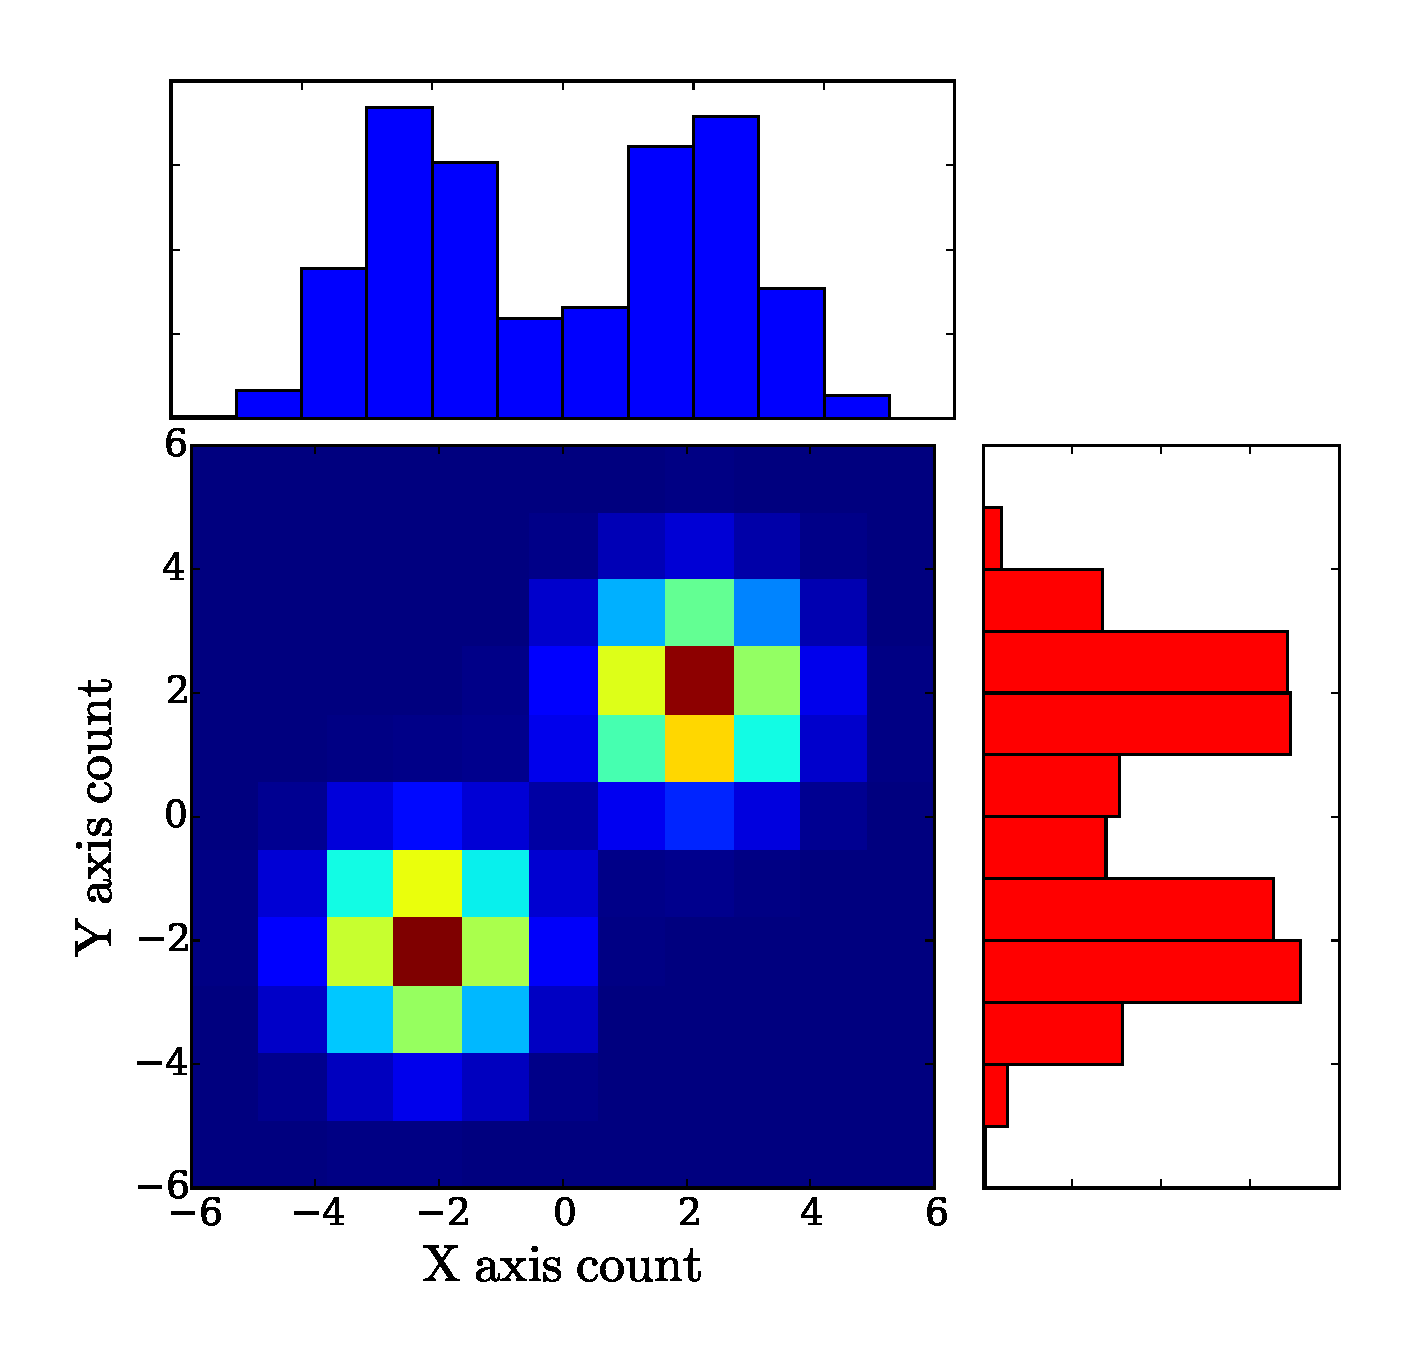
\includegraphics[clip, trim=0.5cm 0.5cm 0.5cm 0.5cm, width=\textwidth]{figure/amb_2and2.pdf}
        \caption{Existe un problema de ambig\"uedad en la reconstrucci�n de posiciones. Dos opciones son igual de factibles.  }
    \end{subfigure}
    ~
    \begin{subfigure}[b]{0.4\textwidth}
        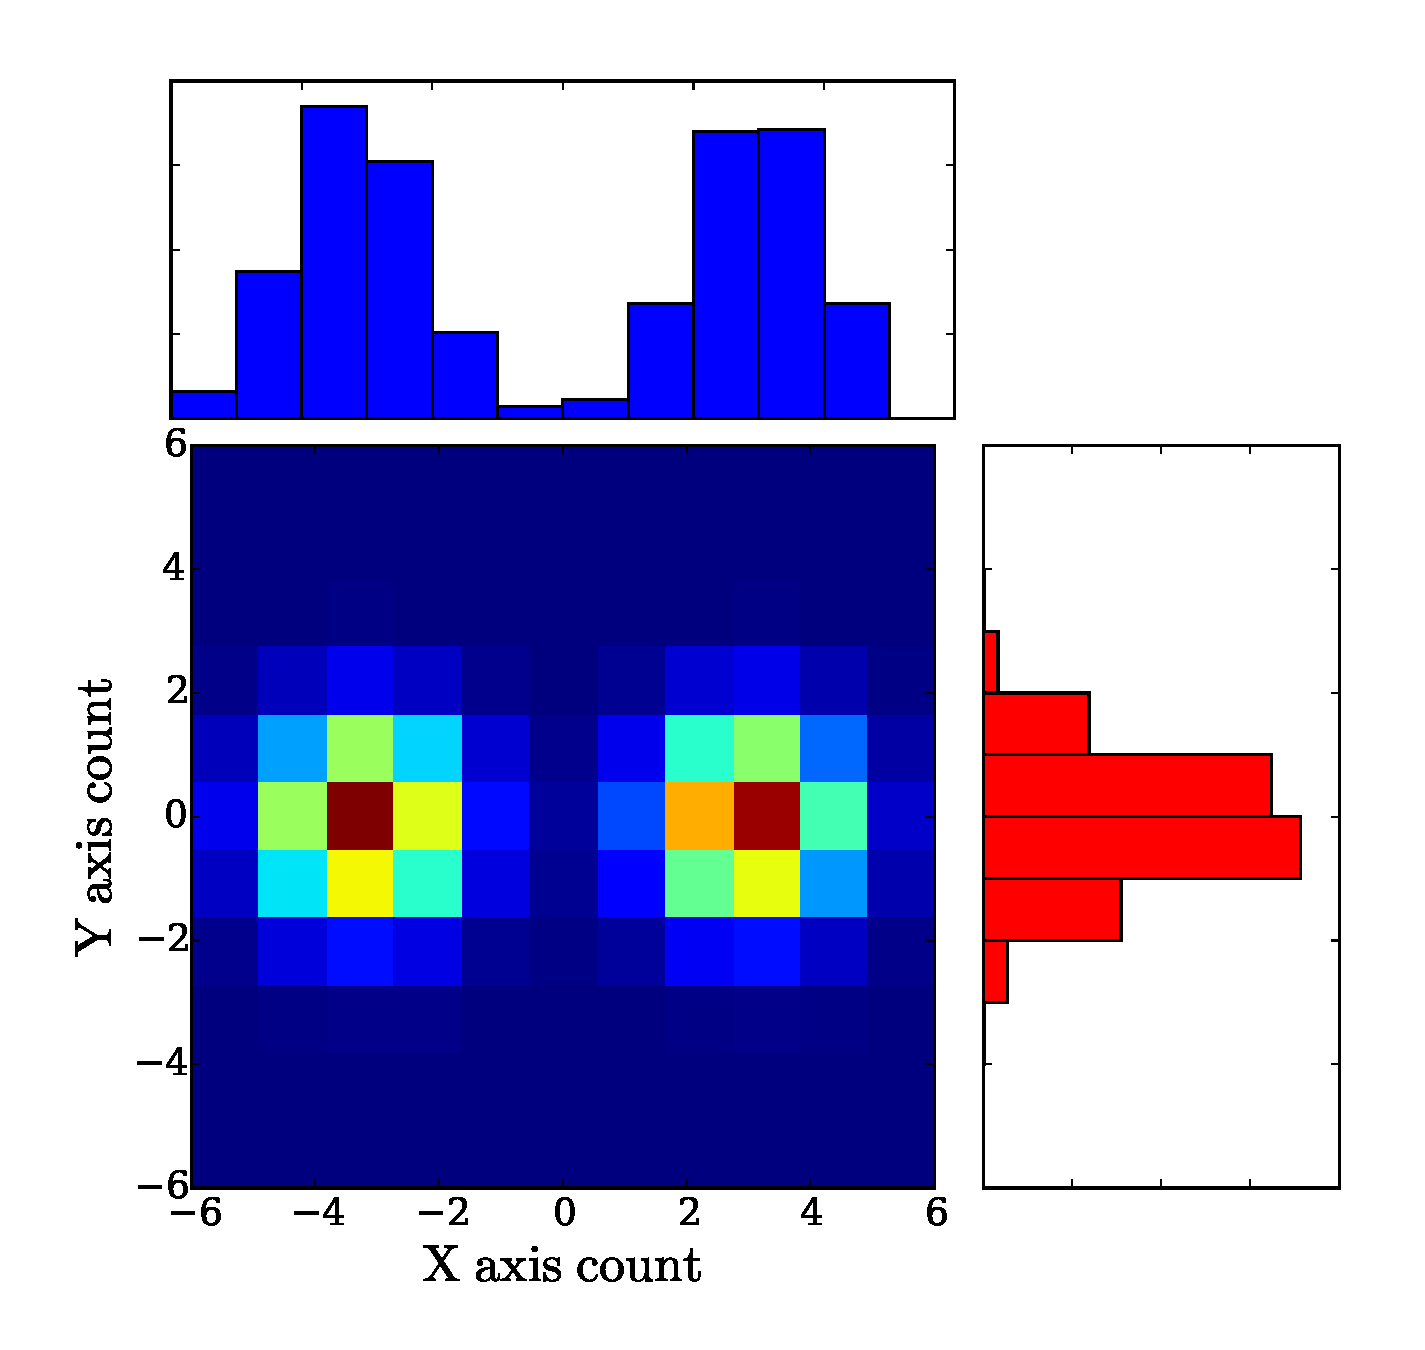
\includegraphics[clip, trim=0.5cm 0.5cm 0.5cm 0.5cm,width=\textwidth]{figure/amb_1and2.pdf}
        \caption{Dos part�culas se observan como una en uno de los ejes debido al solapamiento de las lluvias.}
    \end{subfigure}

    \caption{Diagramas que muestran algunos de los problemas que presenta la particular disposici�n del sistema de lectura del detector preshower.
    Debido a que s�lo se conocen los valores acumulados de conteo en los ejes X e Y, la reconstrucci�n de la posici�n en el plano presenta algunas ambig\"uedades que se deben solucionar. }
    \label{fig:ambig}
\end{figure}


\begin{itemize}
\item Una algoritmo clustering, encargada de identificar y separar cada una de las part�culas detectadas por el detector. Como ya se mencion�, la entrada para este algoritmo depende del sistema de lectura del detector, ya que es el primer paso en el proceso de reconstrucci�n, com�nmente esta entrada son mediciones de energ�a u otro valor en las posiciones (X,Y), sin embargo, en el caso del detector preshower la entrada es distinta por lo que se deben adaptar los algoritmos para ser utilizados en esta situaci�n especial. Com�nmente el conjunto de valores de energ�a o fotoelectrones deben ser agrupados de manera de representar part�culas incidentes. Adem�s es deseable eliminar posibles fuentes de ruido en las lecturas de manera que los cluster obtenidos correspondan a valores correspondientes a se�al.

\item En una segunda fase se deben identificar los m�ximos de cada uno de estos cluster, varios m�ximos indican que m�s de una part�cula corresponden a ese cluster. Estos m�ximos pueden corresponder a la posici�n del lector con mayor conteo de fotoelectrones, sin embargo, este m�todo ingenuo puede tener problemas debido a, por ejemplo, dos lectores vecinos con mediciones altas muy parecidas, adem�s el m�todo es muy sensible al ruido. Otros m�todos mas elaborados pueden ser considerados en este paso.

\item En el caso de identificar varios m�ximos en el mismo cluster es necesario separar la cantidad de fotoelectrones correspondientes a cada una de estas part�culas. El algoritmo para la separaci�n de part�culas solapadas se conoce como algoritmo de \emph{unfolding}. Este algoritmo es capaz de distribuir la energ�a entre ambas part�culas de manera de obtener dos o m�s clusters de energ�as separados que luego ser�n utilizados en el calculo de posici�n o energ�a.

\item Luego de identificar la energ�a correspondiente a cada part�cula para cada uno de los cluster detectados, es necesario reconstruir la posici�n incidente de la part�cula bas�ndose en los valores detectada por el sistema de lectura. El algoritmo de reconstrucci�n de posici�n se encarga de estimar la posici�n de la part�cula incidente utilizando la energ�a depositada y la posici�n de las celdas de cada cluster. La energ�a de la part�cula puede ser estimada luego integrando los valores de cada cluster.
\end{itemize}

El algoritmo completo nos entrega mediciones de energ�a y posici�n para cada una de las part�culas incidentes. Sin embargo hay una diferencia fundamental en el preshower que implica considerar otro paso en el algoritmo de reconstrucci�n. El sistema readout s�lo entrega la informaci�n de la cantidad acumulada de fotoelectrones en cada uno de los ejes transversales, por lo que la medici�n de la energ�a depositada en cada cristal no esta disponible, lo que genera ciertas ambig\"uedades a la hora de separar dos o m�s part�culas. Considerar por ejemplo que dos clusters son observados en el eje X y en el eje Y. Pensar que se reconstruye la posici�n de estos cluster con un m�todo cualquiera, obteni�ndose posiciones $[x_1, x_2]$ en el eje X y $[y_1,y_2]$ en el eje Y. Entonces, tenemos 2 distintas formas de reconstruir la posici�n en el plano, $[(x1,y1),(x2,y2)]$ o $[(x1,y2),(x2,y1)]$. El problema se complica mucho m�s cuando se observan m�s de dos clusters en los ejes, debido a que pueden ocurrir combinaciones como $[(x1,y2),(x2,y2)]$ en casos en que ambas part�culas se observen como un s�lo cluster en un de los ejes, debido a solapamiento de las lluvias. En la Figura~\ref{fig:ambig} se observan ambos casos mencionados. Entonces, se debe agregar un paso encargado de la combinaci�n de clusters entre ambos ejes y la resoluci�n de ambig\"uedades  que pudiesen aparecer al combinar los clusters.  Este es un paso fundamental para el funcionamiento del detector preshower y se analizar� a mas profundidad en la Secci�n~\ref{experimentos}.


En la siguiente secci�n se analizar� las propuestas de la literatura para cada uno de los pasos correspondiente al algoritmo de reconstrucci�n. Si bien, muchas de estas propuestas se realizan en el contexto de detectores con capacidad para medir la posici�n en el plano, no es dif�cil adaptar su funcionamiento al caso uni-dimensional que tratamos en este trabajo. Al conocimiento del autor de esta propuesta, no existe trabajo en algoritmos de reconstrucci�n para una arquitectura similar a la del detector preshower, por lo que mucho de lo propuesto en la Secci�n~\ref{experimentos} ser� trabajo original, pero tomando ideas de los algoritmos de reconstrucci�n propuestos para otros detectores. 



    \chapter{Estado del Arte \label{estado}}
Un algoritmo de reconstrucci�n se compone de varios sub-procesos, que en conjunto permiten reconstruir la energ�a y posici�n de una o m�s part�culas detectadas. Si bien existen varias posibilidades en el proceso de reconstrucci�n, tales como la reconstrucci�n del �ngulo de incidencia, la reconstrucci�n de trayectoria~\cite{speer2006track}, las principales tareas que interesan en este trabajo son: el agrupamiento de los datos, la identificaci�n de m�ximos en los clusters, la identificaci�n y separaci�n (cuando es posible) de part�culas solapadas y la reconstrucci�n de la posici�n y energ�a de cada una de estas part�culas.\\
A continuaci�n se analizar�n cada una de estas tareas por separado.
\section {Clustering de part�culas}
La entrada al algoritmo es la medici�n de cada uno de los lectores del sistema. La estructura de esta entrada depende de la configuraci�n del sistema de lectura, este puede ser capaz de medir la energ�a (o fotoelectrones) depositada en cada celda o s�lo medir una proyecci�n en cada eje de la energ�a depositada (como en el caso del preshower). La entrada depende del sistema de lectura, pero com�nmente corresponde a un conjunto de valores de energ�a o fotoelectrones que deben ser agrupados de manera de representar part�culas incidentes. Las part�culas incidentes usualmente depositan su energ�a en varias celdas o cristales del calor�metro. La finalidad de los algoritmos presentados aqu� es agrupar estas celdas. El algoritmo debe tambi�n eliminar posibles fuentes de ruido en las lecturas en caso de ser posible. El ruido en los calor�metros viene de dos fuentes principales. Primero, ruido es introducido por distintos procesos en la electr�nica de lectura. Segundo, existe ruido conocido como de apilamiento (\emph{pile-up}). Este tipo de ruido proviene de interacciones extras que ocurren al mismo tiempo que la part�cula atraviesa el detector.

Varios m�todos han sido propuestos en la literatura para formar los clusters en calor�metros basados en cristales. Entre los algoritmos propuestos se pueden encontrar m�todos de construcci�n incremental de los clusters que funcionan muy bien en la pr�ctica, tambi�n es posible encontrar algoritmos m�s avanzados que utilizan m�todos probabil�sticos para construir los clusters. 

En lo que continua analizaremos algunos de los algoritmos m�s utilizados en el trabajo de clustering en detectores con geometr�as relativamente similar al detector preshower. 

\subsection{Ventana deslizante}
Este algoritmo es propuesto por el experimento ATLAS y es utilizado en el proceso de reconstrucci�n del calor�metro electromagn�tico y el calor�metro hadr�nico~\cite{lampl2008calorimeter}. Los clusters pueden utilizar informaci�n combinada de ambos calor�metros, esto es �til para reconstruir jets e identificaci�n de leptones Tau o utilizar solo la informaci�n del calor�metro electromagn�tico, �til para la reconstrucci�n de electrones y fotones.  

El detector calor�metro en atlas se compone tanto de secciones longitudinales como secciones transversales, las secciones longitudinales se extienden en el espacio $\eta - \sigma$, y existen cuatro secciones transversales en el caso del calor�metro electromagn�tico: \emph{middle}, \emph{strips}, \emph{pre-sampler} y \emph{back}.

El algoritmo se compone de tres pasos principales: construcci�n de torres, b�squeda de pre-clusters y llenado de clusters. 

\subsubsection{Construcci�n de torres}
El espacio longitudinal $\eta-\sigma$ es segmentado en $N_{\eta}\times N_{\phi}$ celdas de tama�o $\Delta \eta \times \Delta \phi$ formando torres transversales de celdas donde la energ�a depositada es sumada. Los valores $N_{\eta}$ y $N_{\phi}$ son definidos como par�metros del algoritmo y deben ser seleccionados de antemano. Si existen celdas que corresponden a m�s de una torre, entonces la energ�a de las celdas es repartida en en proporci�n al �rea de la celda en cada torre.

\subsubsection{B�squeda de pre-clusters}
 Se define una ventana de tama�o fijo $N^{window}_{\eta} \times N^{window}_{\phi}$ en unidades del tama�o de torre $\Delta \eta \times \Delta \phi$. La ventana es movida a lo largo de las torres construidas y pre-clusters son formados en los m�ximos locales de energ�a acumulada en la torre (definida como la suma de energ�as en todas las celdas que forman parte de la torre) que, adem�s, superen un umbral $E_T^{thresh}$.
 
 La posici�n en el eje $\eta-\phi$ de los pre-clusters obtenidos en este paso es calculada utilizando el centro de masa con pesos iguales a la energ�a en cada una de las celdas incluidas en las torres. Es posible tambi�n definir tama�os menores para las ventanas utilizadas al calcular la posici�n, es decir utilizar $N^{pos}_{\eta} \times N^{pos}_{\phi}$, esto con la finalidad de minimizar el ruido introducido en el calculo de posici�n.
 
 Finalmente, este paso termina removiendo los clusters duplicados. Estos se definen como dos pre-clusters que tengan posiciones centrales dentro de $\Delta \eta_{dupl} \times \Delta \phi_{dupl}$. S�lo el pre-clusters con mayor cantidad de energ�a integrada es conservado.
 
\subsubsection{Llenado de clusters}

En el caso de estar trabajando en la formaci�n de clusters combinados con informaci�n conjunta del calor�metro hadr�nico y electromagn�tico, los cluster corresponden a los pre-clusters formados en el paso anterior. Para el caso de la construcci�n de clusters electromagn�ticos, se definen diferentes tama�os de clusters para cada una de las capas del calor�metro, esto debido a que el campo electromagn�tico en el detector afecta de manera diferente a las part�culas que pasan por el calor�metro en diferentes capas de este. Los nuevos cluster son construidos bas�ndose en las posiciones calculadas para los pre-clusters. Adem�s se pueden definir clusters de distintos tama�os dependiendo de la part�cula hipotetizada. Nose ahondar� mucho en esto �ltimo debido a que es muy espec�fico al funcionamiento del detector calor�metro de ATLAS.

Este algoritmo es utilizado en el detector atlas para la reconstrucci�n de electrones y fotones~\cite{aad2012electron,atlas4calorimeter} y la reconstrucci�n de leptones Tau~\cite{kalinowski2009tau} (aunque en versiones actuales del algoritmo esto se cambi� a clustering topol�gico).


%El algoritmo de ventana deslizante que se basa en sumar la energ\'ia (n\'otese que no necesariamente se trata de energ\'ia, puede ser conteo de foto-electrones u otra medida, de aqu\'i en adelante se utilizar\'a energ\'ia para simplificar la explicaci\'on) en celdas dentro de un rect\'angulo de tama\~no fijo. La posici\'on central del rect\'angulo es seleccionada de manera de maximizar la cantidad de energ\'ia contenida. Este algoritmo es utilizado en el detector ATLAS para la reconstrucci\'on de lluvias electromagn\'eticas~\cite{lampl2008calorimeter}~\cite{atlas4calorimeter}.

\subsection{Cluster topol�gico}

Otro m�todo de clustering utilizado en el experimento ATLAS es el cluster topol�gico~\cite{lampl2008calorimeter,atlas2016topological}. Este algoritmo permite construir clusters de tama�o variable, a diferencia del algoritmo anterior con el que s�lo se pod�an construir clusters de tama�o fijo. El algoritmo consiste de tres pasos principales: b�squeda de semillas, b�squeda de vecinos, construcci�n de clusters.
\subsubsection{B�squeda de semillas}
El algoritmo comienza con la b�squeda de semillas para construir los clusters. Se identifican las celdas con un valor se�al a ruido mayor a un umbral $t_{seed}$ definido de antemano. El valor de se�al se define como el valor absoluto de la energ�a en la celda y otro valor equivalente, mientras que el ruido corresponde al valor esperado del ruido en base a consideraciones electr�nicas y f�sicas. Cada celda seleccionada en este paso corresponde a un proto-cluster.
\subsubsection{B�squeda de vecinos}
La lista de semillas es ordenada en orden descendente bas�ndose en el valor de la raz�n se�al a ruido. Entonces, por cada semilla en orden se consideran las celdas vecinas que superen un umbral $t_{cell}$. Si el vecino no esta en la lista de utilizados y supera el umbral entonces es agregado a un proto-cluster correspondiente a la semilla. Si la celda es adyacente tambi�n a otro proto-cluster entonces ambos son combinados. Si la celda agregada adem�s supera un umbral $t_{neighbor}$ entonces la celda es utilizada como semilla para expandir el cluster. Esto asegura que las colas de las lluvias electromagn�ticas no sean descartadas pero al mismo tiempo asegura que no se agregue ruido electr�nico y de apilamiento. El proceso continua hasta procesar todas las semillas de la lista original, continuando luego con las semillas agregadas por los vecinos en el paso anterior. Esto continua hasta que no quedan m�s semillas. 
\subsubsection{Construcci�n de clusters}
Como paso final, los proto-clusters que quedan del paso anterior (algunos fueron combinados) son ordenados de mayor a menor (respecto a la energ�a u otro valor equivalente) y convertidos en clusters. Adicionalmente se pueden eliminar los que tengan energ�a total $E_t$ menor a un umbral $t_E$, con la finalidad de evitar clusters construidos de ruido.

Notar que es posible que los clusters obtenidos con el algoritmo de clustering topol�gico correspondan a m�s de una part�cula incidente, debido al solapamiento de lluvias (para el clustering por ventana deslizante se asume que cada cluster de tama�o fijo corresponde a s�lo una lluvia). Por lo anterior, es necesario agregar un paso de divisi�n de clusters, esto se tratar� en la secci�n~\ref{solapamiento}. 

El algoritmo de cluster topol�gico ha sido utilizado extendidamente en la reconstrucci�n de jets y MTE (\emph{missing transverse momentum}) en los calor�metros electromagn�tico y hadr�nico de ATLAS~\cite{pinfold2012evaluation,barillari2008local,cojocaru2004hadronic}, mostrando una gran eficiencia en la reconstrucci�n~\cite{atlas2016topological}.

\subsection{Fuzzy c-means}
Otro m�todo exitosamente aplicado en la literatura es el algoritmo de clustering fuzzy c-means. K-means es una muy popular t�cnica de clustering que aprende de manera no supervisada a encontrar K clusters en los datos. Su uso es muy extendido en la miner�a de datos y se extiende por las mas variadas disciplinas. Para el trabajo de reconstrucci�n de part�culas en detectores calor�metros, esta t�cnica (y en general cualquier t�cnica de clustering duro) no es adecuada ya que asigna cada dato a un s�lo cluster, lo que no permite lluvias solapadas, que como ya se vio son muy comunes. Los m�todos fuzzy, en cambio, permiten que cada punto pertenezca en menor o mayor grado a diferentes clusters. Estos m�todos combinan los algoritmos de clustering b�sicos con la teor�a fuzzy [FUZZY] que permite agregar conceptos de imprecisi�n e incerteza a los m�todos duros. El algoritmo fuzzy c-means, en espec�fico, es una versi�n fuzzy del algoritmo K-means. Existen estudios de la aplicaci�n de este algoritmo para reconstrucci�n de part�culas en calor�metros~\cite{FUZZY,PRESHOWER}, sin embargo, al conocimiento de este autor no hay aplicaciones reales (en detectores) de este algoritmo.

En ~\cite{FUZZY} el algoritmo fuzzy c-means y una extensi�n de este, el algoritmo dynamic fuzzy c-means, es aplicado para la reconstrucci�n en datos simulados de un detector calor�metro de muestreo. En este trabajo se demuestra la utilidad de los algoritmos fuzzy en la tarea de reconstrucci�n debido a la capacidad de estos m�todos de manejar las lluvias solapadas autom�ticamente. 

Fuzzy c-means comienza con un conjunto de datos $X = (x_1, x_2, ..., x_N)$ con $x_i \in \mathbb{R}^d$, para estos datos busca el conjunto de clusters con centros $V = (v_1, v_2, ..., v_C)$ con $v_i \in \mathbb{R}^d$ que minimicen la funci�n de costo 
\begin{equation}
J_m (U,V;X) = \sum_{k=1}^N \sum_{i=1}^C (u_{ik})^m||x_k - v_i||^2, \nonumber
\end{equation}
donde $U$ consiste de los valores $u_{ik}$ que corresponden a los grados de pertenencia de el punto $k$ al cluster $i$, $||x|| = \sqrt{x^Tx}$ es la norma de producto interno y el valor $m\in[1,\infty[$ (factor fuzzy) define el grado de fucificaci�n del algoritmo, donde $m$ cercano a $1$ corresponde a un simple k-means. Imponiendo restricciones 
\begin{align}
\sum_{k=1}^N u_{ik} > 0, i \in \{1,...,C\} \nonumber \\
\sum_{i=1}^C u_{ik} = 1, k \in \{1,...,N\}. \nonumber
\end{align}	
Es posible resolver el problema iterando el siguiente algoritmo
\begin{equation}
u_{ik} = \bigg[\sum_{j=1}^C\bigg(\frac{D_{ik}}{D_{jk}}\bigg)^{\frac{2}{m-1}}\bigg]^{-1}, \nonumber
\end{equation}
con $D_{ik} = ||x_k - v_i|| > 0$ para todo $i$ y $k$. Y
\begin{equation}
v_i = \frac{\sum_{k=1}^n(u_{ik})^m x_k}{\sum_{k=1}^n(u_{ik})^m}. \nonumber
\end{equation}
El algoritmo procede alternando las estimaciones de $V$ y $U$ hasta alcanzar un n�mero definido de iteraciones o alcanzar un umbral de error $\epsilon$ definido de ante mano.




    \chapter{Experimentos \label{experimentos}}

\section{Introducci�n}
En esta secci�n se presentan resultados del algoritmo de reconstrucci�n para simulaciones del detector Preshower. Los estudios que se realizan mediante simulaciones corresponden a:
\begin{itemize}
\item Reconstrucci�n de posici�n y an�lisis de errores sistem�ticos en la reconstrucci�n de posici�n.
\item Separaci�n de lluvias solapadas utilizando el algoritmo de unfolding.
\item Identificaci�n de lluvias solapadas en casos en que el algoritmo de separaci�n de lluvias sea incapaz de identificar dos part�culas.
\item Resoluci�n de ambig�edades para m�s de una part�cula incidentes.
\item Estudios de resoluci�n energ�tica y de posici�n para diferentes separaciones entre part�culas incidentes.
\end{itemize}

\section{Simulaciones}
Para estudiar la performance del algoritmo de reconstrucci�n en el detector preshower, el detector ha sido simulado utilizando GEANT 4~\cite{agostinelli2003geant4}. El prototipo simulado corresponde a un arreglo de 25x25 cristales LYSO. Cada cristal tiene un tama�o cd 4x4x45 mm$^3$. Los cristales est�n cubiertos por una pintura reflectora en la cara trasera para evitar fuga de fotones por la cara no sensible. En la cara frontal de la matriz de cristales una placa de acr�lico de ancho igual a 1.5 mm es posicionada. Esta placa esta cubierta por un material reflector en su cara frontal para evitar la fuga de fotones. En la placa se posicionan 25 fibras horizontales y 25 fibras verticales de 1 mm de di�metro que pasan por el centro de cada cristal. Estas fibras tambi�n est�n cubiertas por materiales reflectantes en las esquinas no sensitivas para evitar la fuga de fotones. Los MPPC son reemplazados por materiales sensibles que pemiten medir los fotones que llegan al sistema de lectura. Toda la geometr�a esta cubierta por placas de aluminio de 2.5 mm de espesor con uniones de cobre. Una simulaci�n de la geometr�a completa del detector es mostrada en la Figura~\ref{fig:detector_completo}.

\begin{figure}
    \centering
    \begin{subfigure}[b]{0.4\textwidth}
        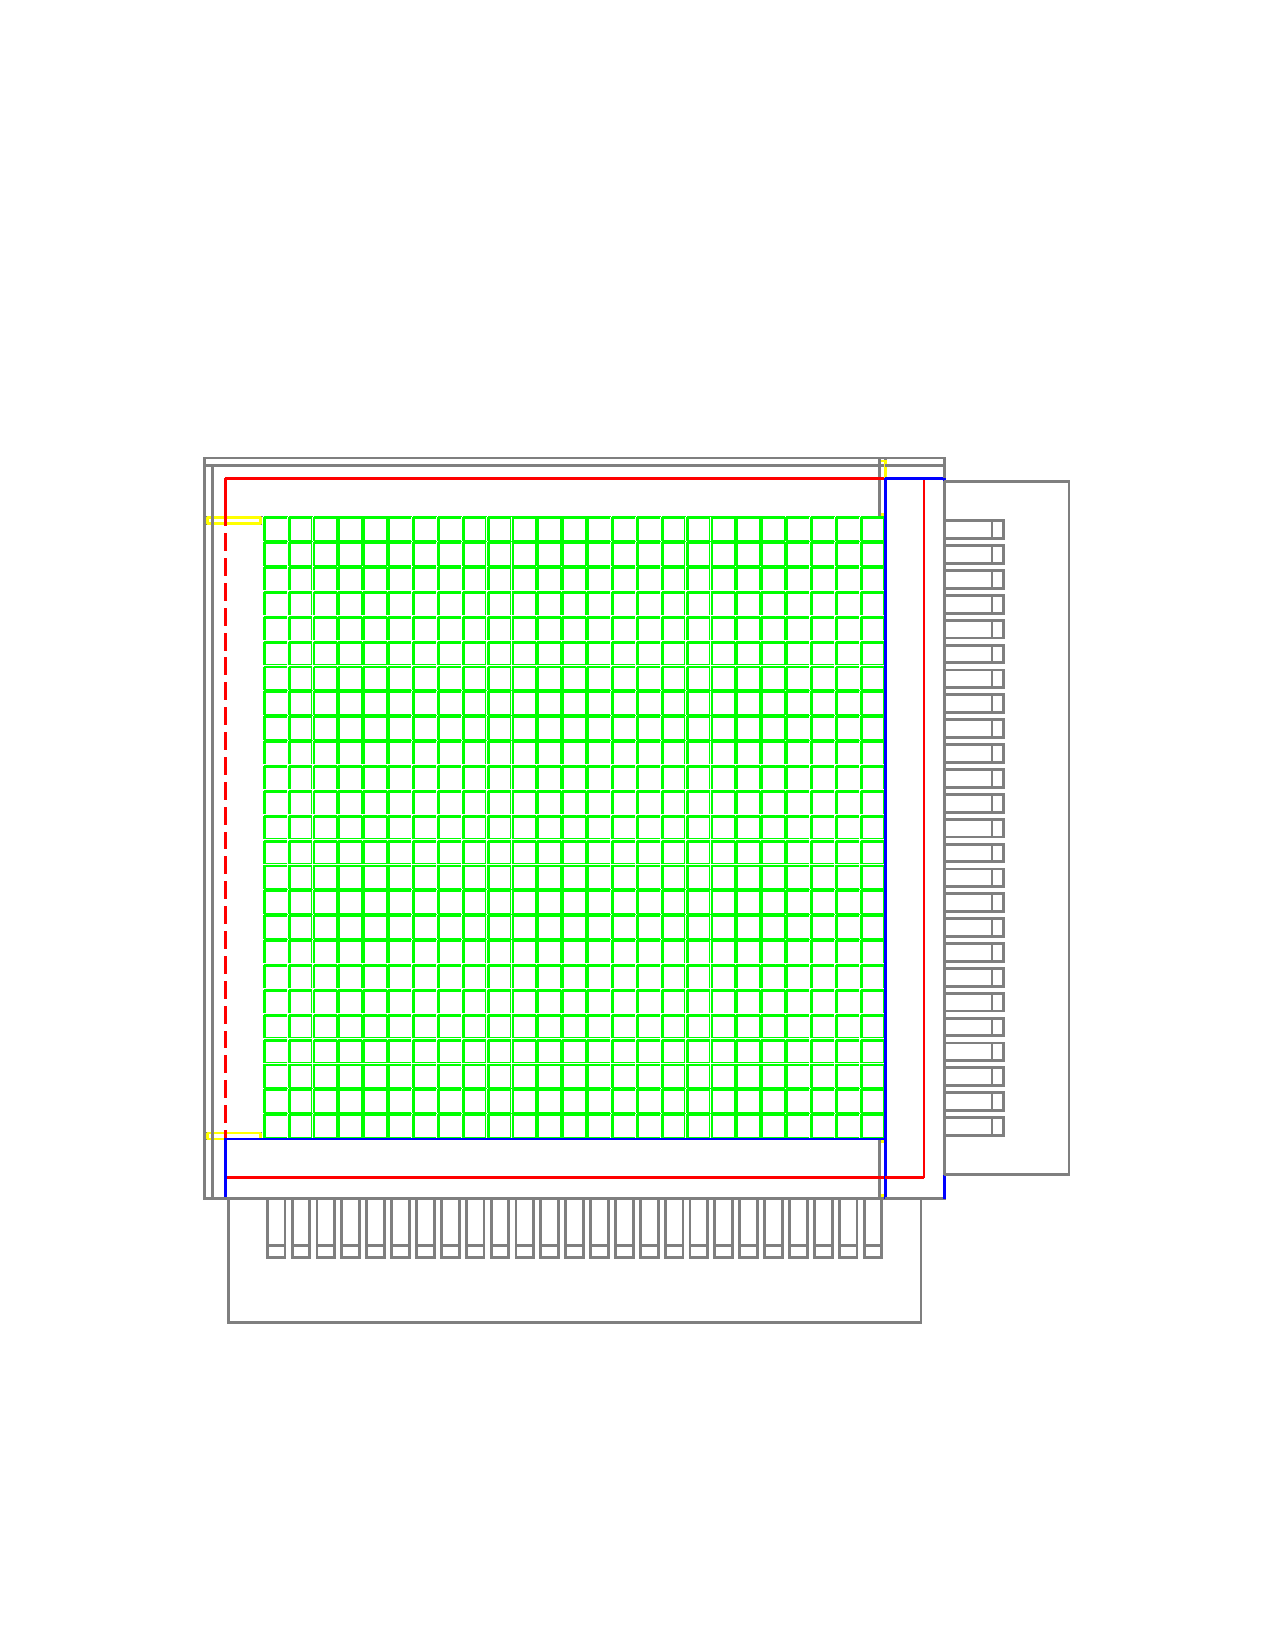
\includegraphics[clip, trim=0.5cm 0.5cm 0.5cm 5.5cm, width=\textwidth,angle=90]{figure/detector-2.pdf}
        \caption{Cara frontal.}
    \end{subfigure}
    ~
    \begin{subfigure}[b]{0.42\textwidth}
        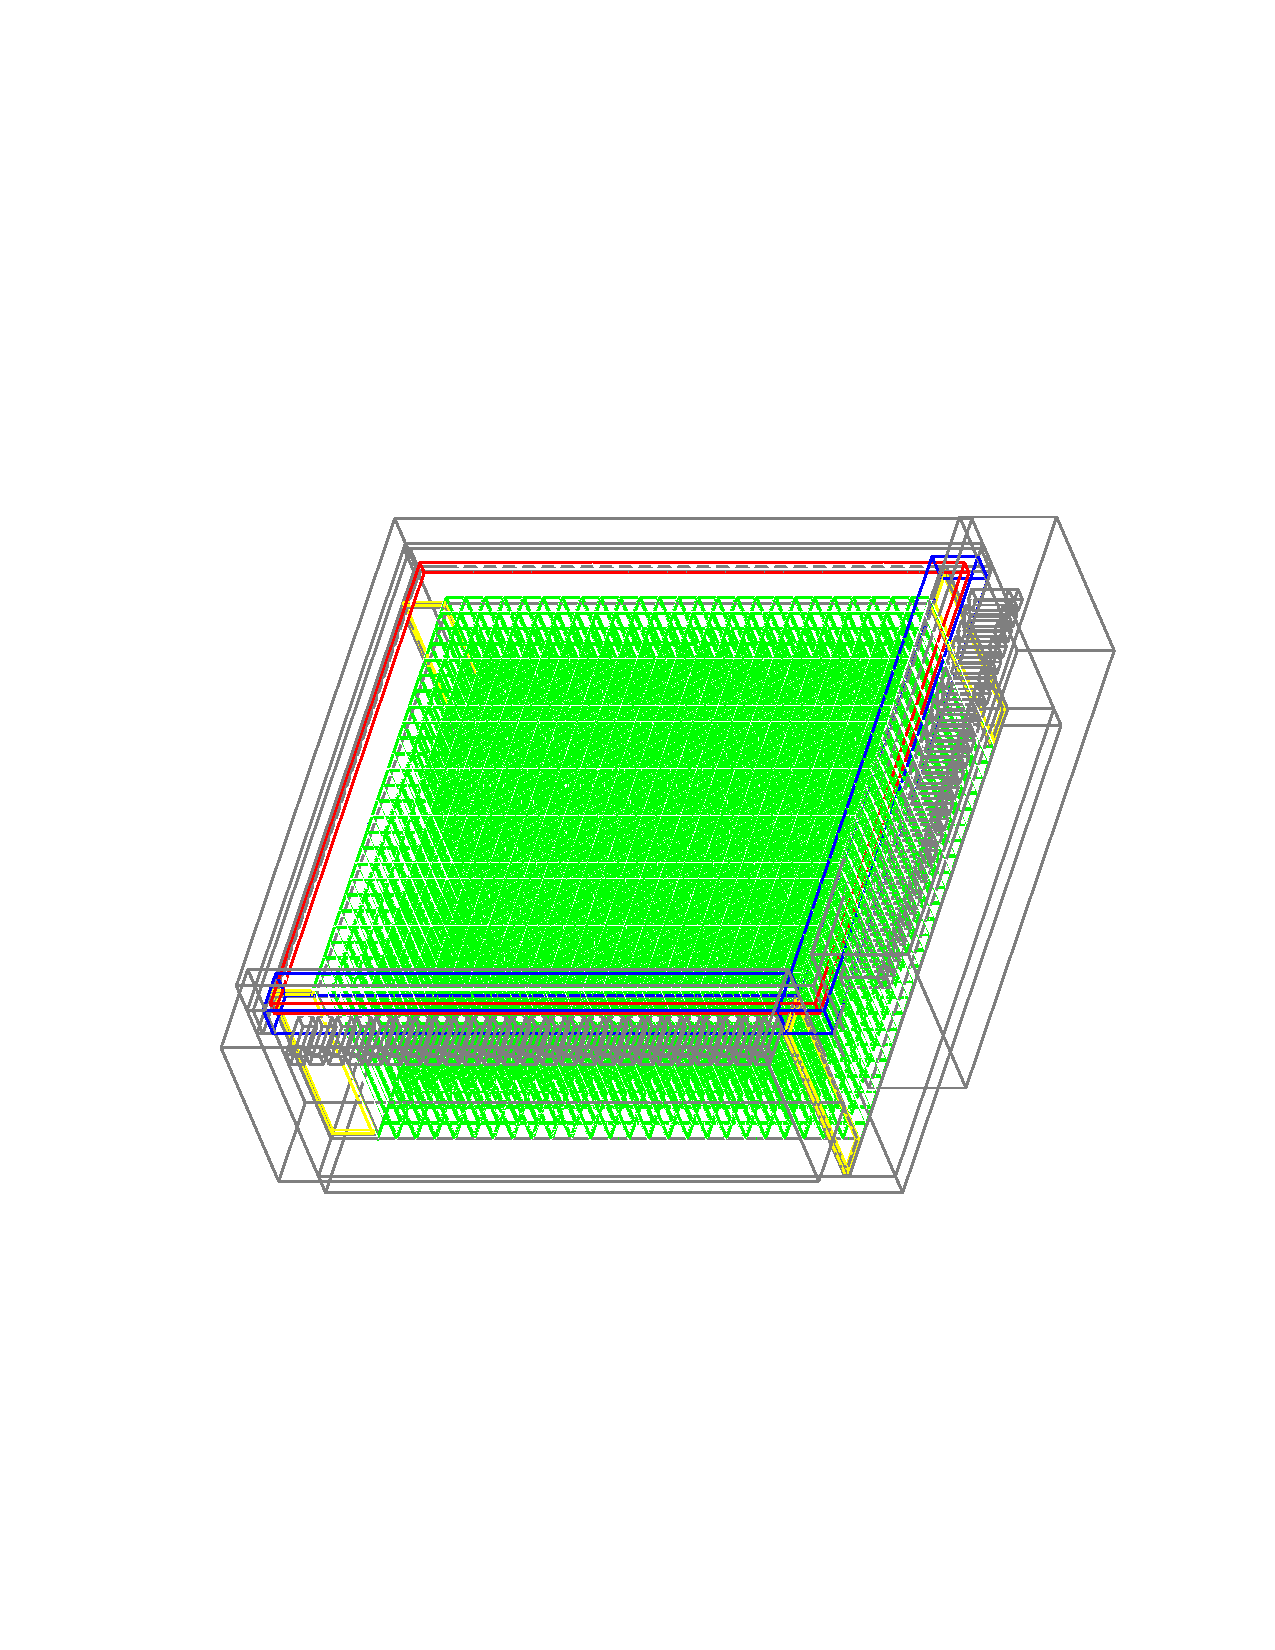
\includegraphics[clip, trim=2.5cm 7.5cm 0.5cm 0.5cm,width=\textwidth,angle=90]{figure/detector-1.pdf}
        \caption{Perspectiva rotada.}
    \end{subfigure}

    \caption{Geometr�a del detector preshower completa simulada. Mostrado en verde se observa la matriz de cristales, en plomo el material cobertor de la matriz y el sistema de lectura, en rojo se muestra la placa de acr�lico en la que se montan las fibras de luz (no mostradas para facilitar la visualizaci�n de los componentes).}
    \label{fig:detector_completo}
\end{figure}

 La geometr�a ha sido simplificada con la finalidad de acelerar el lento proceso de simulaci�n en los experimentos para la reconstrucci�n. Muchos de los elementos exteriores del detector (como la cubierta protectora) no fueron considerados. Estos elementos se utilizan principalmente para evitar influencia de factores externos que no est�n presentes en las simulaciones. Adem�s, la matriz de fibras para la lectura y el sistema de lectura es removido para evitar el lento trabajo de simulaci�n de los procesos en las fibras. En su lugar la respuesta obtenida por el panel de lectura es aproximada usando un modelo estad�stico basado en mediciones reales que permite obtener la cantidad aproximada de fotones que llegan a cada MPPC en base a la energ�a medida en cada cristal. Para obtener el modelo estad�stico utilizado para simular la salida de cada MPPC dada la energ�a medida en cada cristal se asume que la cantidad de fotoelectrones que llegan a cada MPPC es una funci�n de Poisson de la suma de energ�a que llegan al MPPC desde cada cristal. La energ�a que llega al MPPC desde cada cristal se modela como una distribuci�n gaussiana centrada en la posici�n del cristal en el eje correspondiente al MPPC normalizada seg�n el valor de energ�a depositada en el cristal. En t�rminos matem�ticos, los valores $p_{xl}$ y $p_{yk}$ correspondientes a la salida de la fibra $l$ y $k$ en el eje $x$ e $y$ respectivamente se calculan en base a las energ�as $E_{ij}$ correspondientes al cristal $(i,j)$. Primero se calculan los valores $u^l_{ij}$, $u_{ij}^k$ como: 
\begin{eqnarray}
u_{ij}^{l} = 20 \cdot E_{ij} \cdot \bigg[\frac{1}{2\sqrt{2\cdot\pi\cdot4}}\exp\bigg(\frac{-(l - i)^2}{2\cdot4}\bigg)\bigg],\\
u_{ij}^{k} = 15 \cdot E_{ij} \cdot \bigg[\frac{1}{2\sqrt{2\cdot\pi\cdot6.25}}\exp\bigg(\frac{-(k - j)^2}{2\cdot6.25}\bigg)\bigg],\nonumber
\label{eq:modelo}
\end{eqnarray}
entonces, $p_x^l$ y $p_y^k$ las salidas de las fibras $l$ y $k$ en los eje $x$ e $y$ son calculados como
\begin{eqnarray}
p_x^l = Poiss\big(\sum_{ij} u_{ij}^{l}\big),\nonumber\\
p_y^k = Poiss\big(\sum_{ij} u_{ij}^{k}\big).\nonumber
\end{eqnarray}
 
Estas salidas corresponden al conteo de foto electrones detectado por el MPPC $l$ o $k$.
 En la Figura~\ref{fig:detector_min} se muestra la versi�n simplificada del detector en conjunto a la interacci�n de dos part�culas $\gamma$ incidentes.
 
\begin{figure}
    \centering
    \begin{subfigure}[b]{0.4\textwidth}
        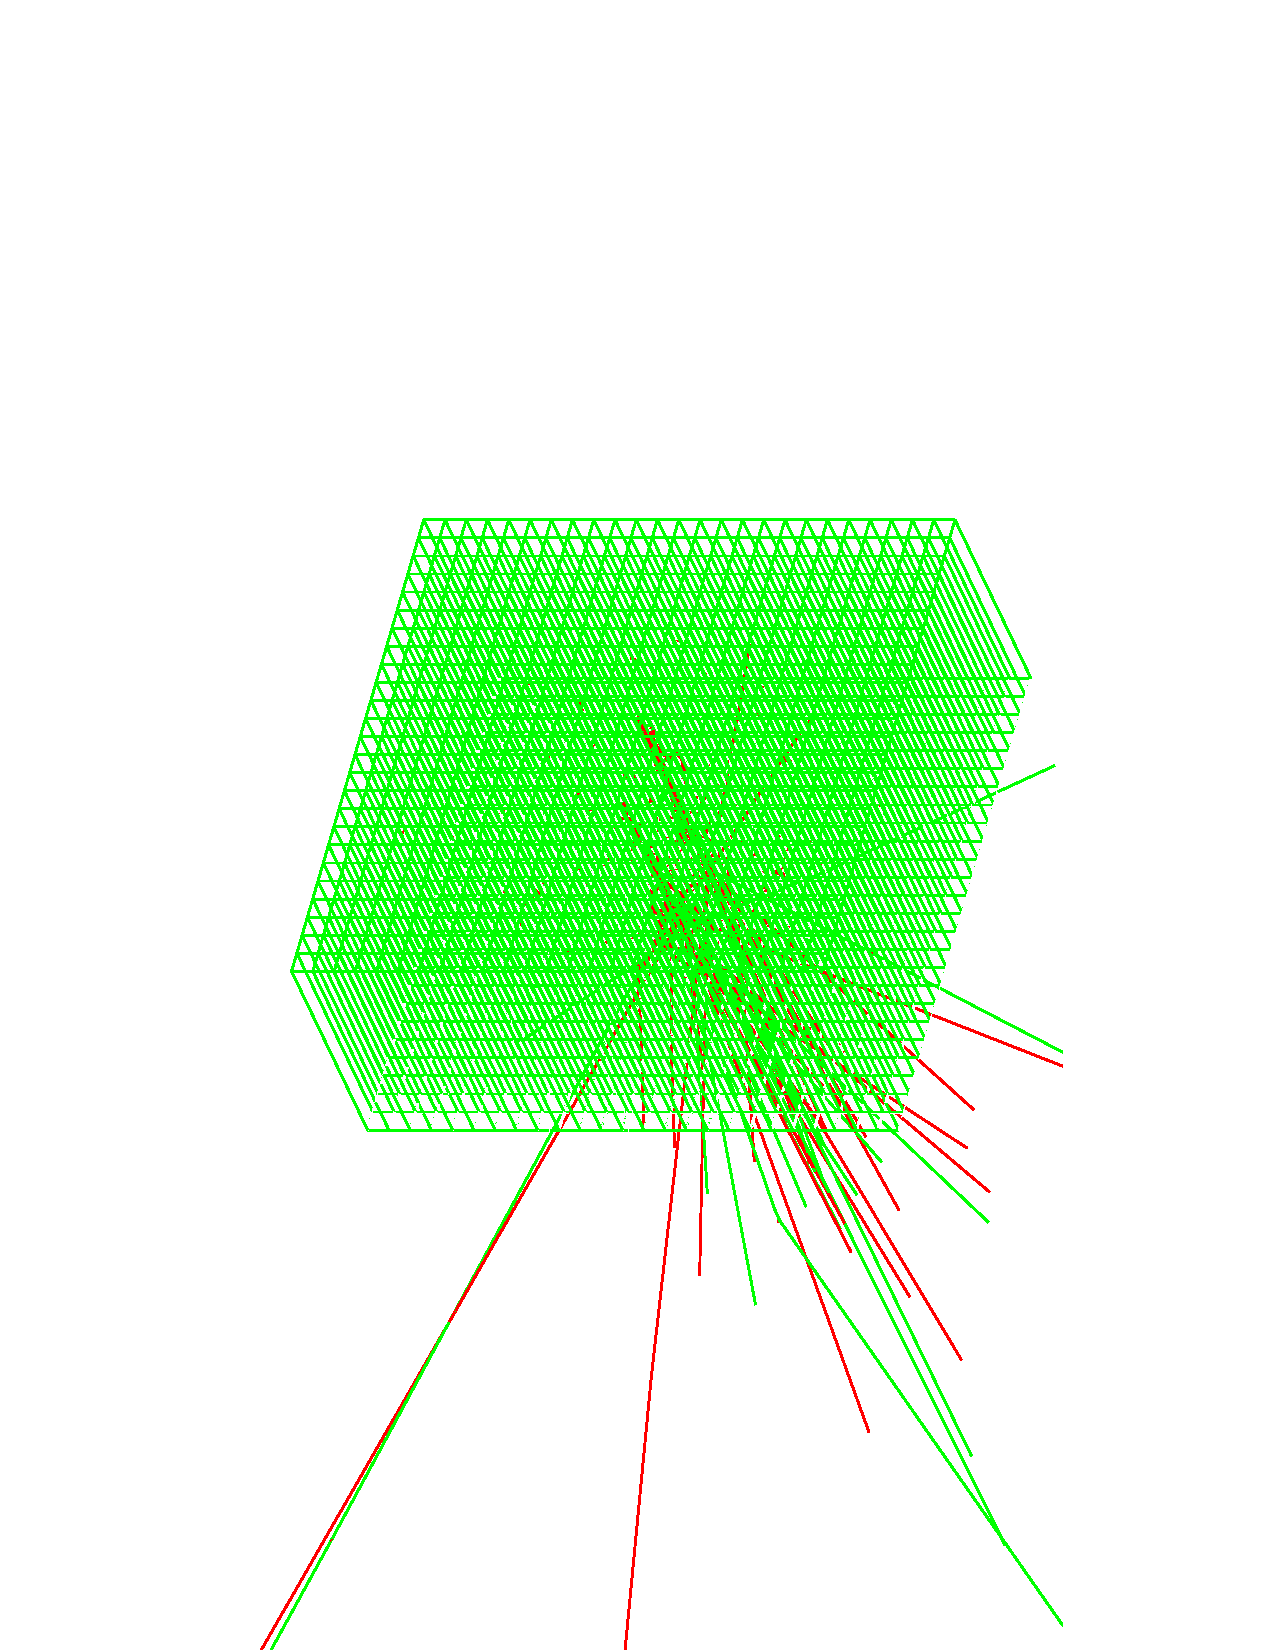
\includegraphics[clip, trim=0.5cm 0.5cm 0.5cm 5.5cm, width=\textwidth,angle=90]{figure/interaction_2.pdf}
        \caption{Perspectiva rotada.}
    \end{subfigure}
    ~
    \begin{subfigure}[b]{0.42\textwidth}
        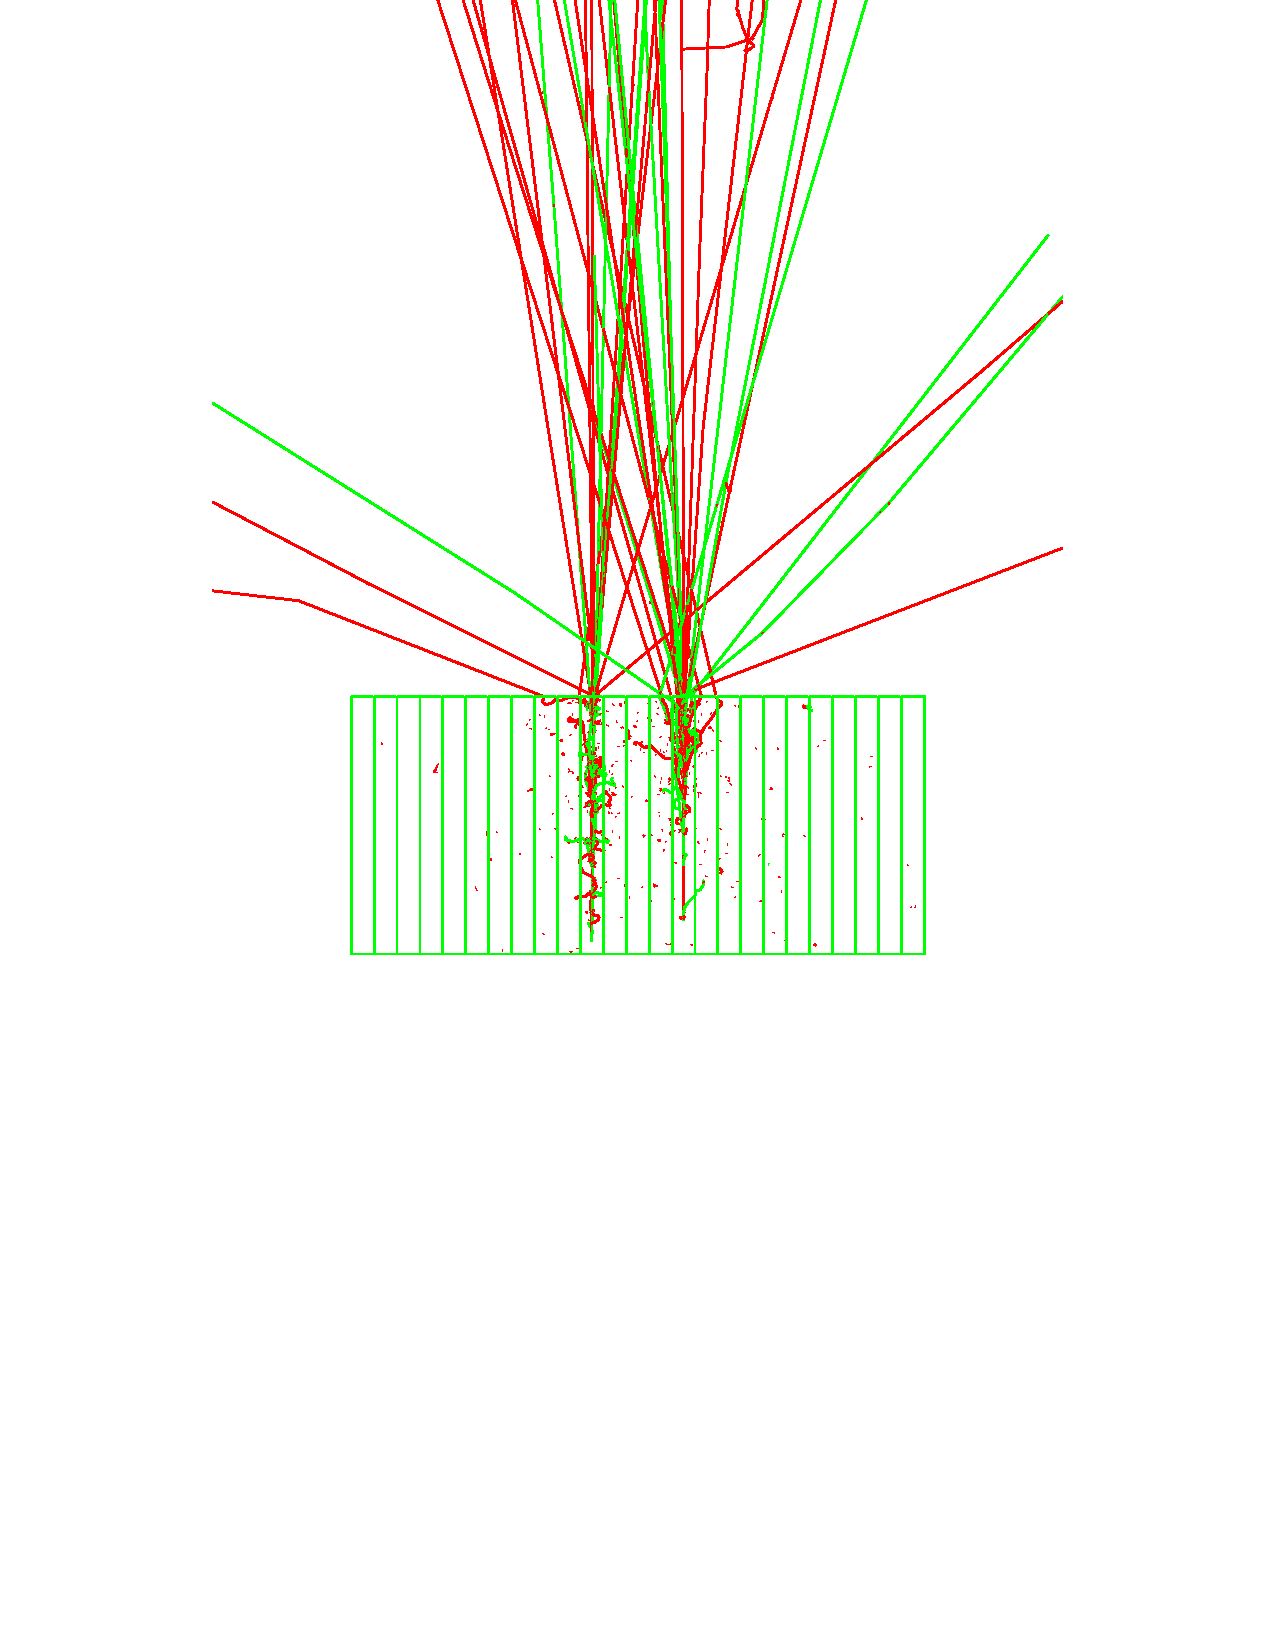
\includegraphics[clip, trim=2.5cm 7.5cm 0.5cm 0.5cm,width=\textwidth,angle=90]{figure/interaction_1.pdf}
        \caption{Cara superior.}
    \end{subfigure}

    \caption{Geometr�a simplificada del detector preshower, donde s�lo se simula la matriz de cristales del detector. En la imagen se muestra la matriz en verde y la interacci�n de dos part�culas $\gamma$ incidentes de 5 GeV. Las trayectorias de los electrones son mostradas en rojo mientras que las trayectorias de positrones son mostradas en verde.}
    \label{fig:detector_min}
\end{figure}

Los experimentos fueron realizados en el rango 0.5-10 GeV. Se consider� un valor de ruido de 2.25 MeV, este valor fue seleccionado en base a la eficacia del algoritmo de clustering para identificar clusters correctamente en el rango de energ�a mencionado anteriormente (este valor es mucho menor que los valores utilizados en la literatura~\cite{alice1999technical}, debido al tama�o considerablemente menor de los cristales para el detector preshower). Los experimentos fueron realizados utilizando part�culas $\gamma$, lanzadas distribuidas de manera uniforme e en el cuadrado central de 80x80 cm de la matriz de cristales (esto para evitar casos especiales en los cuales las part�culas inciden muy cerca de los l�mites, en los cuales cierta energ�a es perdida provocando algunos problemas en la reconstrucci�n).

\section{Algoritmo de reconstrucci�n}
En esta secci�n se presenta el algoritmo de reconstrucci�n propuesto para el detector preshower y se estudia la eficacia en la reconstrucci�n de part�culas mediante simulaciones. Debido a que el foco principal del detector preshower es detectar part�culas $\gamma$ muy cercanas entre s�, que com�nmente provienen del decaimiento de un pi�n neutro, especial cuidado se debe tomar en los siguientes puntos:
\begin{itemize}
\item Identificaci�n de lluvias electromagn�ticas provenientes de part�culas gammas individuales. Reconstrucci�n de posici�n de incidencia y energ�a depositada de estas part�culas.
\item Reconocimiento y separaci�n de part�culas $\gamma$ solapadas, especialmente para el caso de dos part�culas muy cercanas (el caso del pi�n neutro). 
\item Rechazo de part�culas solapadas en casos en que estas no puedan ser separadas. Esto, para evitar reconocer las part�culas como un solo fot�n en casos en que no sea as�.
\end{itemize}
El algoritmo completo de reconstrucci�n consiste de los siguientes procesos
\begin{enumerate}
\item Construcci�n de clusters.
\item Identificaci�n de m�ximos en los clusters.
\item Separaci�n de lluvias solapadas.
\item Reconstrucci�n de posici�n y energ�a.
\item Resoluci�n de ambig�edades.
\end{enumerate}

\subsection{Algoritmo de clustering}
El algoritmo de clustering es el paso principal del algoritmo de reconstrucci�n. Para el detector preshower se decidi� utilizar el algoritmo topol�gico presentado en la Secci�n~\ref{topol�gico}. El algoritmo de clustering topol�gico es un algoritmo muy utilizado en la pr�ctica y permite la construcci�n de clusters de tama�os variables (a diferencia del algoritmo de ventana deslizante), lo que es importante para el detector preshower, debido a que la profundidad menor de los cristales provoca una gran variabilidad en la cantidad de energ�a depositada en cada evento (esto a causa de que muchas de las part�culas interact�an en la secci�n final del cristal, depositando s�lo una parte de su energ�a). Otras opciones, como el algoritmo de clustering fuzzy, fueron rechazadas debido a la poca o nula utilizaci�n en experimentos reales de estos algoritmos y debido a que no utilizan toda la informaci�n disponible en el preshower (en el caso del algoritmo de clustering fuzzy, no se hace uso de la informaci�n disponible en la distribuci�n lateral de la matriz de cristales).

El algoritmo de clustering topol�gico implementado para el detector preshower se resume en el Algoritmo~\ref{alg:algtopologico}.
\begin{algorithm}
\caption{Algoritmo de clustering}
\label{alg:algtopologico}
\begin{algorithmic}[1]
\State Como entrada se tiene dos arreglos de valores para cada celda y para cada eje (X e Y).
\Procedure{Adyacentes}{celda,cluster}
  \For{Cada vecino de la celda}
  	\State{A�adir vecino a cluster}
	\State{Marcar celda de vecino como usado}
	\State{Llamar Adyacentes(vecino,cluster)}
  \EndFor
\EndProcedure
\For{Cada eje }
	\State {El arreglo de conteos es llenado con los valores mayores a \emph{cut1} en el eje correspondiente.}
	\State {El arreglo de conteos es ordenado de mayor a menor y todos los valores son inicializados como no usados. }
	\For{Cada valor en el arreglo de conteos}
		\If{Si valor es mayor a \emph{cut2} y el valor no esta marcado como usado}
			\State{Crear nuevo cluster}
			\State{A�adir posici�n como semilla de un cluster, marcar celda como usada.}
			\State{Llamar Adyacentes(semilla,cluster)}
		\EndIf
	\EndFor
\EndFor

\end{algorithmic}
\end{algorithm}

Los valores \emph{cut1} y \emph{cut2} corresponden al umbral de ruido y a un umbral �til para identificar m�ximos respectivamente. Estos valores fueron elegidos observando la eficacia del algoritmo de clustering para identificar part�culas en el umbral 0.5-10 GeV. Sin embargo, se nota que el algoritmo es relativamente robusto a variaciones (no muy grandes) de estos valores. Los valores usados son $cut1 = 2.25$ y $cut2 = 3.75$. 

Notar que el algoritmo no es exactamente igual al algoritmo topol�gico presentado en la Secci�n ~\ref{topol�gico}. De este se ha quitado, primero, la recombinaci�n de clusters, debido a que de la separaci�n de lluvias adyacentes y solapadas se encarga el algoritmo de unfolding y segundo, se ha quitado el umbral utilizado en la decisi�n de utilizar el vecino como semilla o no, en cambio todos los vecinos son utilizados como semilla. Esto �ltimo debido a que las colas de la lluvia son muy importantes para lograr una buena reconstrucci�n en el detector preshower.
Teniendo los clusters identificados, el algoritmo continua con la b�squeda m�ximos locales en cada uno de los clusters por separado. 

\subsection{B�squeda de m�ximos}
El siguiente paso del algoritmo es la b�squeda de m�ximos en cada uno de los clusters encontrados. El an�lisis posterior depende de la cantidad de m�ximos encontrados en cada cluster. En caso que se encuentre s�lo un m�ximo, entonces se considera que el cluster ha sido originado por una sola lluvia o puede ser originado por m�s de una lluvia pero imposibles de separar. En este caso se analiza, en caso de ser posible, si el cluster proviene de m�s de una part�cula, si no, la posici�n de la part�cula incidente y su energ�a puede ser reconstruida. Si el cluster posee dos o m�s m�ximos, entonces se considera una superposici�n de lluvias electromagn�tica y el algoritmo de unfolding es aplicado con la finalidad de separar las lluvias. 

\begin{figure}[t]
\makebox[\textwidth][c]{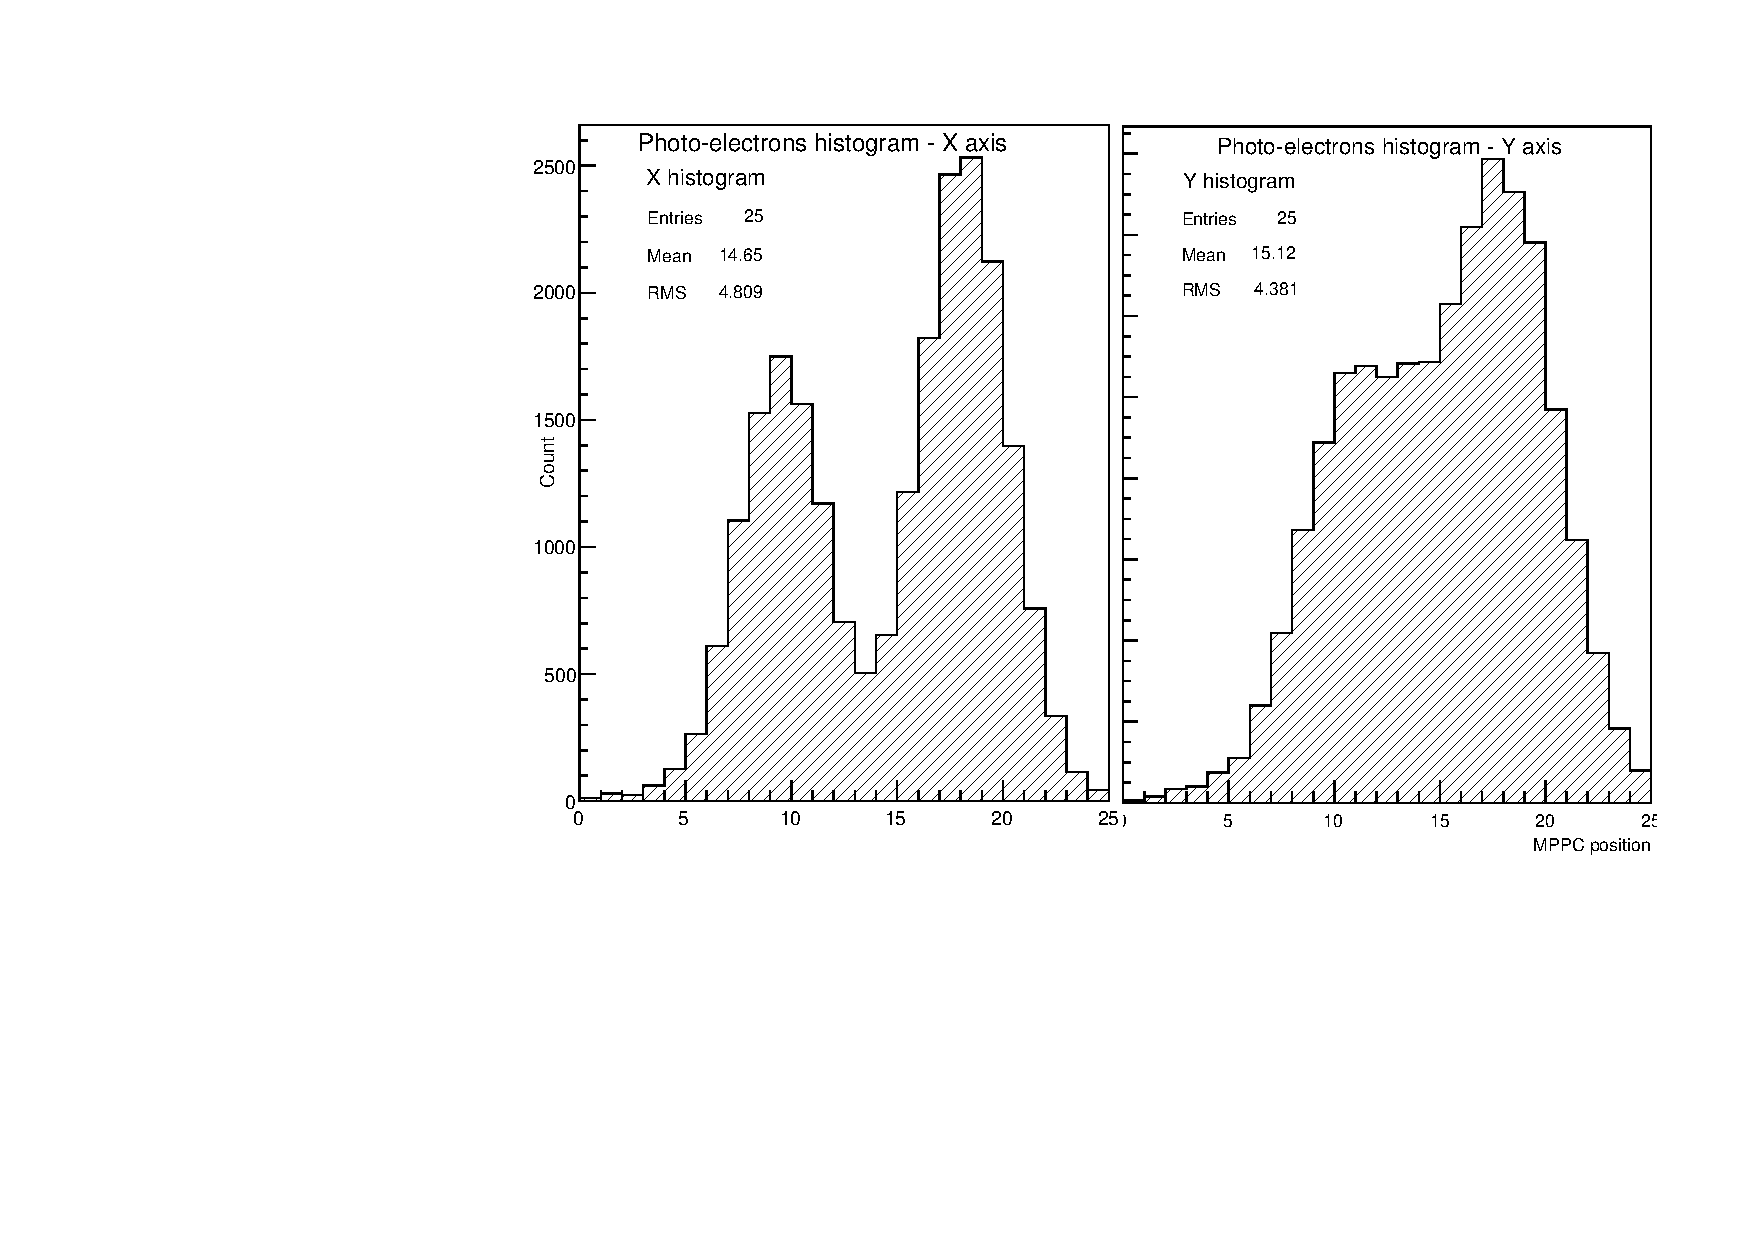
\includegraphics[width=15cm]{figure/plot1_2.pdf}}
%{\centering 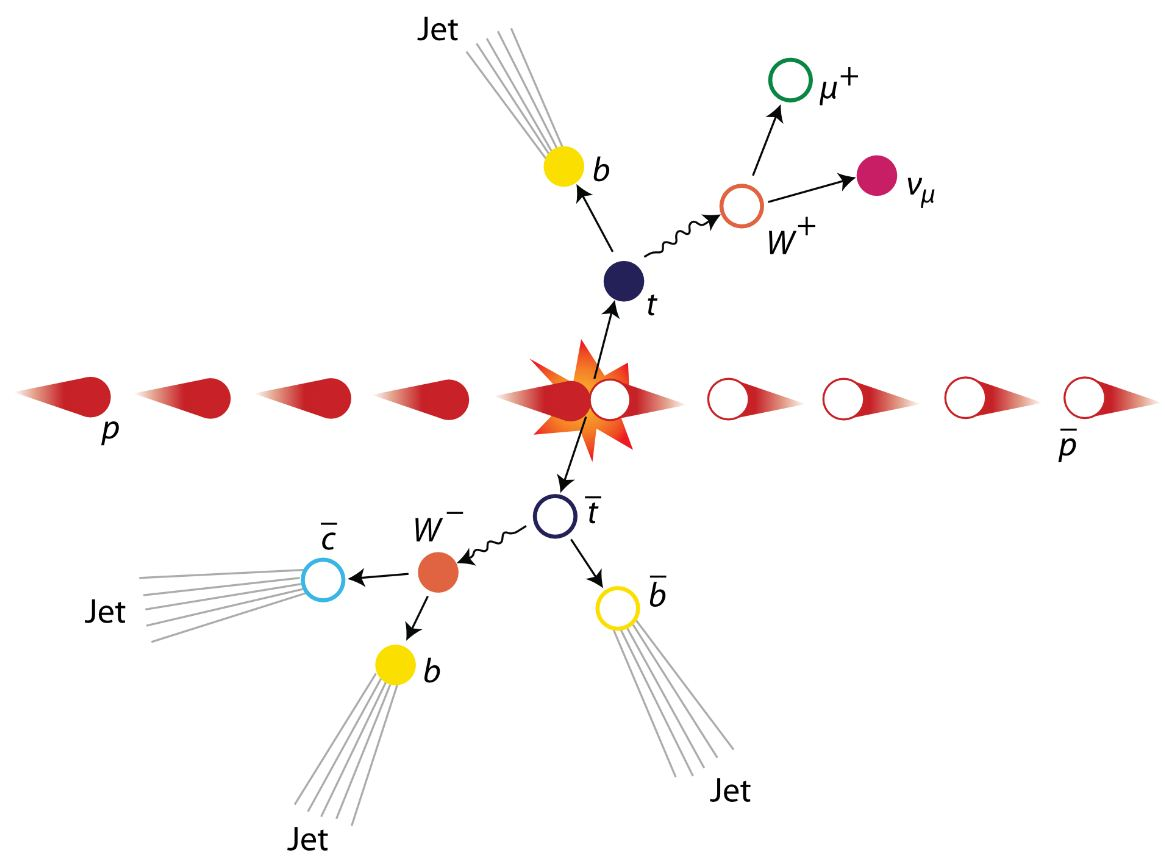
\includegraphics[width=10cm]{figure/collision.JPG}}
\caption[Dos]{Histograma de photo-electrones para cada uno de los ejes para un evento de dos gamas incidentes de 5 GeV. Se observa que la part�cula incidente alrededor de la posici�n 11 del eje Y es muy dif�cil de identificar como un m�ximo, ya que no produce un m�ximo local f�cilmente identificable.\label{fig:dosmaximos}}
\end{figure}

Es posible identificar los m�ximos asignando reglas simples que funcionen en la mayor�a de los casos. En~\cite{alice1999technical} se revisan los valores mayores a un umbral y si el valor de esta celda es adem�s mayor a todos sus vecinos por una cantidad definida con anterioridad, entonces la celda es identificada como m�ximo local. Sin embargo, para el detector preshower el problema es considerablemente m�s complicado. Debido a la relativamente baja probabilidad de interacci�n en el detector preshower, la cantidad de energ�a depositada en cada evento es muy variable (a diferencia de un detector con una profundidad de varias longitudes de radiaci�n, donde la mayor�a de las part�culas interact�an). Debido esto, la definici�n de umbrales a priori para identificar los m�ximos es complicada. Adem�s, debido al di�metro menor de los cristales en el preshower, se dan muchos casos como el mostrado en la Figura~\ref{fig:dosmaximos} (varios cristales comparten gran parte de la energ�a, imposibilitando la identificaci�n de m�ximos locales), en los que ser�a imposible identificar un m�ximos utilizando las reglas simples mencionadas con anterioridad.

Debido a lo anterior, se ha decidido utilizar el algoritmo presentado en la Secci�n~\ref{maximos}. La versi�n utilizada del algoritmo es la del paquete ROOT~\cite{antcheva2009root}, en la clase \emph{TSpectrum}. Si bien el algoritmo se basa principalmente en el algoritmo presentado en~\cite{mariscotti1967method} y su versi�n para varias dimensiones presentada en~\cite{morhavc2000identification}, se agregan algunos pasos extra. Primero, se agrega un paso extra de suavizado, basado en utilizar la distribuci�n estacionaria de una cadena de markov, que asigna mayor probabilidades a las celdas en que se encuentran los peaks, como se menciona en~\cite{silagadze1996new}, este m�todo suaviza y al mismo tiempo intensifica los peaks de la distribuci�n original. Adem�s, se agrega un filtro para los peaks encontrados, que s�lo retorna los peaks que tienen una amplitud mayor a $threshold\times 100 \%$ de el mayor peak. El valor de threshold y el $\sigma$ utilizado en el algoritmo presentado en~\ref{maximos} son definidos como argumentos de la funci�n, para el detector preshower se definieron valores de $\sigma = 2$ y $threshold = 0.05$ (estos son los valores por default, no se encontr� mayor diferencia al variar estos valores alrededor del default). En la Figura~\ref{fig:peaks} se muestra el algoritmo de b�squeda de peaks funcionando para un caso dif�cil del detector preshower.

\begin{figure}[t]
\makebox[\textwidth][c]{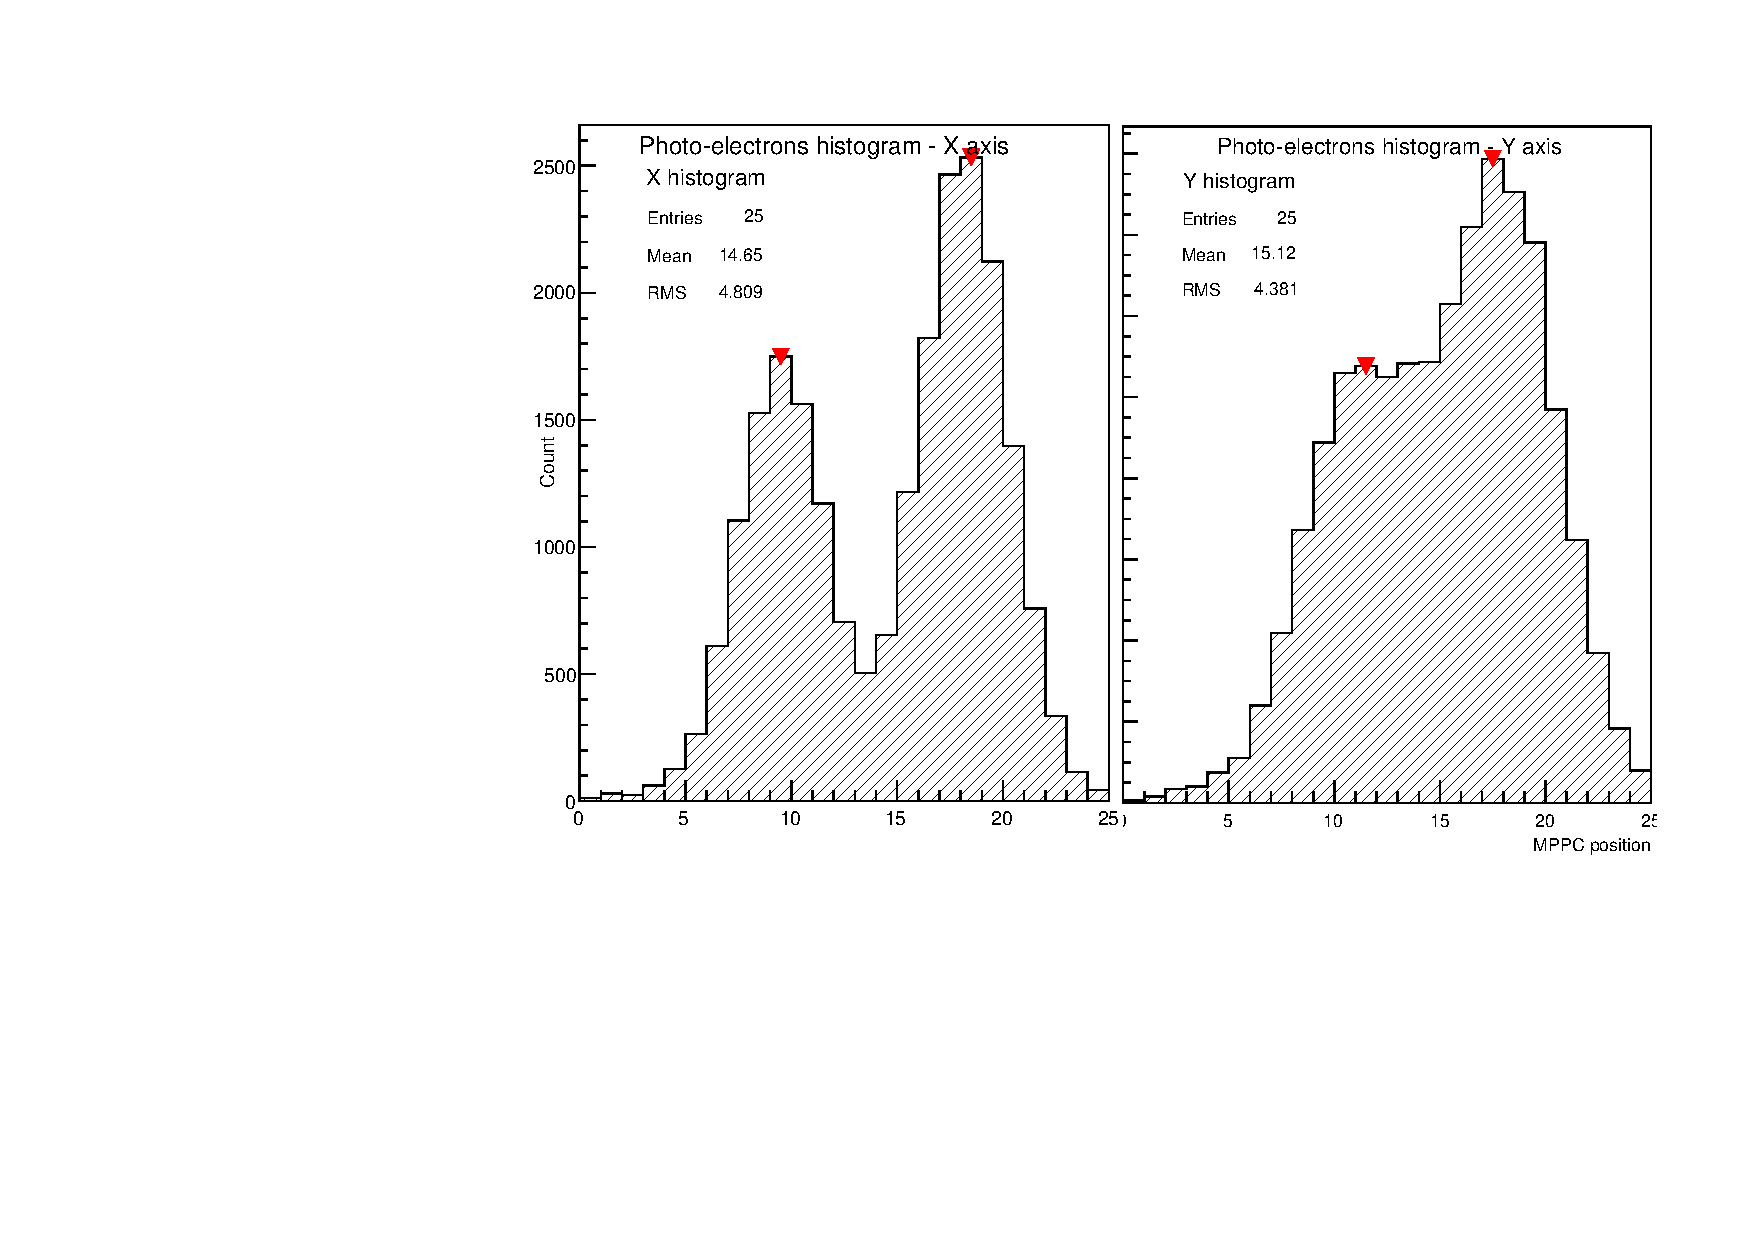
\includegraphics[width=15cm]{figure/plot2_2.pdf}}
%{\centering 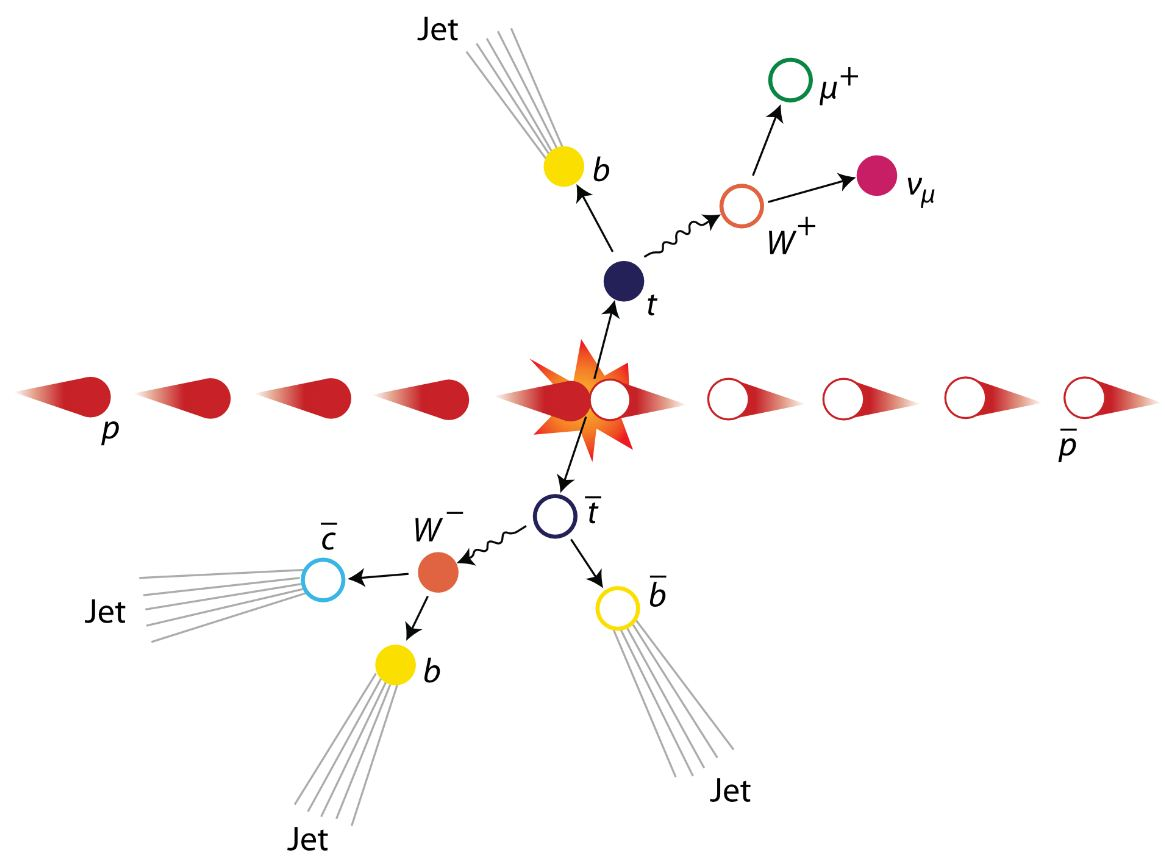
\includegraphics[width=10cm]{figure/collision.JPG}}
\caption[Dos]{Histograma de photo-electrones para cada uno de los ejes para un evento de dos gamas incidentes de 5 GeV. El algoritmo de b�squeda de m�ximos identifica todas las part�culas incidentes en cada eje de manera exitosa, incluso para el caso dif�cil del eje Y.\label{fig:peaks}}
\end{figure}

\subsection{Algoritmo de unfolding}
El m�todo a utilizar para la separaci�n de lluvias solapadas es el presentado en la Secci�n~\ref{solapamiento}. El m�todo se basa en el conocimiento de la distribuci�n lateral de la lluvia en los cristales, por lo que primero la distribution de respuesta lateral unidimensional debe ser calculada y parametrizada para ser usada en la separaci�n de la energ�a depositada en celdas solapadas. La distribuci�n lateral puede ser calculada mediante simulaciones. Para esto se simularon 2500 eventos, cada uno correspondiente a un gamma de 10 GeV lanzado en las dos celdas centrales. Entonces, el conteo de foto-electrones en una celda vs la distancia entre el centro de la celda y la posici�n incidente es graficado. La funci�n obtenida se muestra en la Figura~\ref{fig:lateral}. Sobre estos datos se ajusta la funci�n~\ref{eq:lateral} que provee una parametrizaci�n sobre los datos.  
\begin{eqnarray}
f(r,E) = \begin{cases} A \cdot \exp(-0.09 \cdot r^{1.89})  & r <  26\\
 A' \cdot \exp(-0.1 \cdot r) & r \geq 26 \end{cases},
\label{eq:lateral}
\end{eqnarray}
donde $r$ es la distancia de la celda a la posici�n incidente en cm, $A$ es una constante de normalizaci�n que corresponde al conteo estimado de fotoelectrones de la lluvia. Las simulaciones entregan curvas laterales muy similares para diferentes gamas con diferentes energ�as, por lo que la dependencia en $E$ de la funci�n esta s�lo contenida en el par�metro de normalizaci�n. El ajusta se realiza utilizando el paquete \emph{Minuit} del framework \emph{Root}~\cite{antcheva2009root}. Los errores en cada uno de los bins en el histograma corresponden al error est�ndar en la media $\sigma / \sqrt{n}$.

\begin{figure}[t]
\makebox[\textwidth][c]{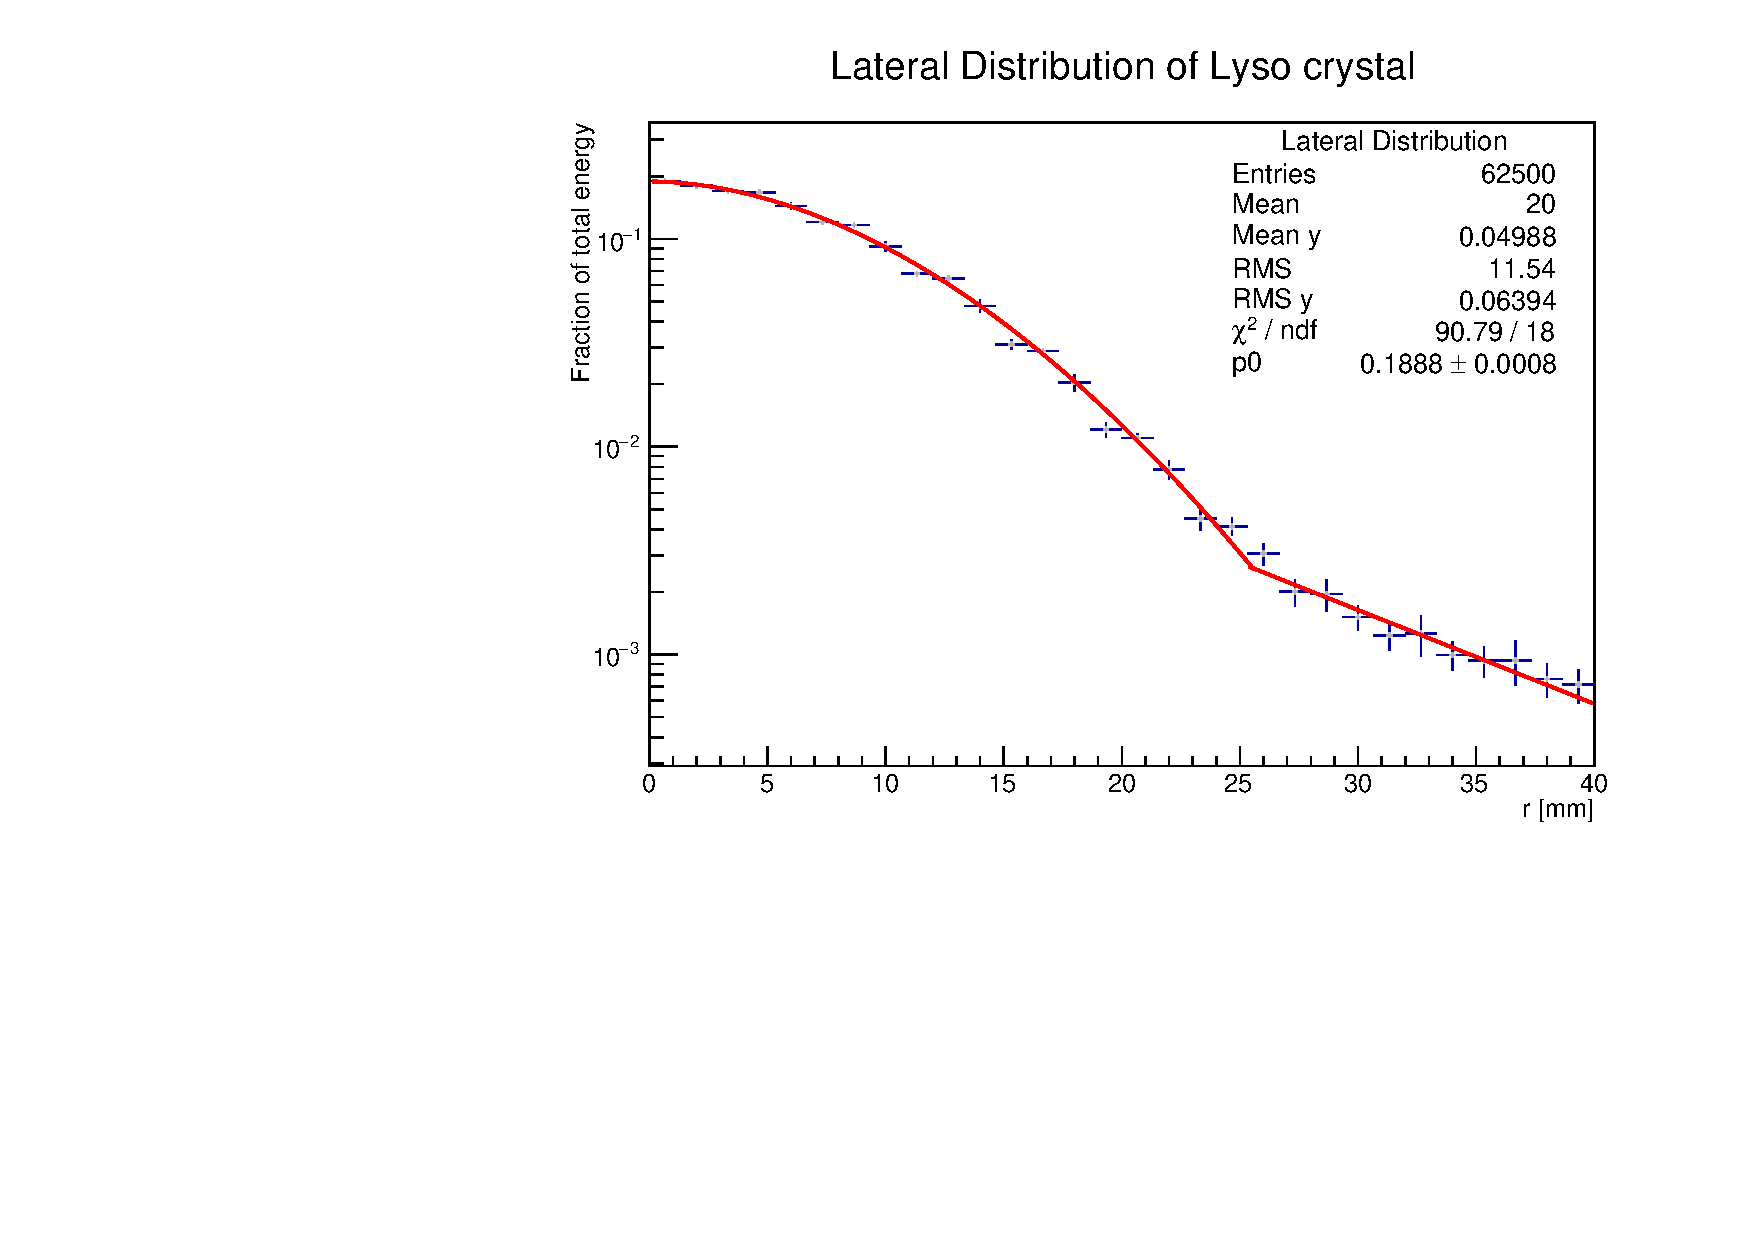
\includegraphics[width=15cm]{figure/lateralfit.pdf}}
%{\centering 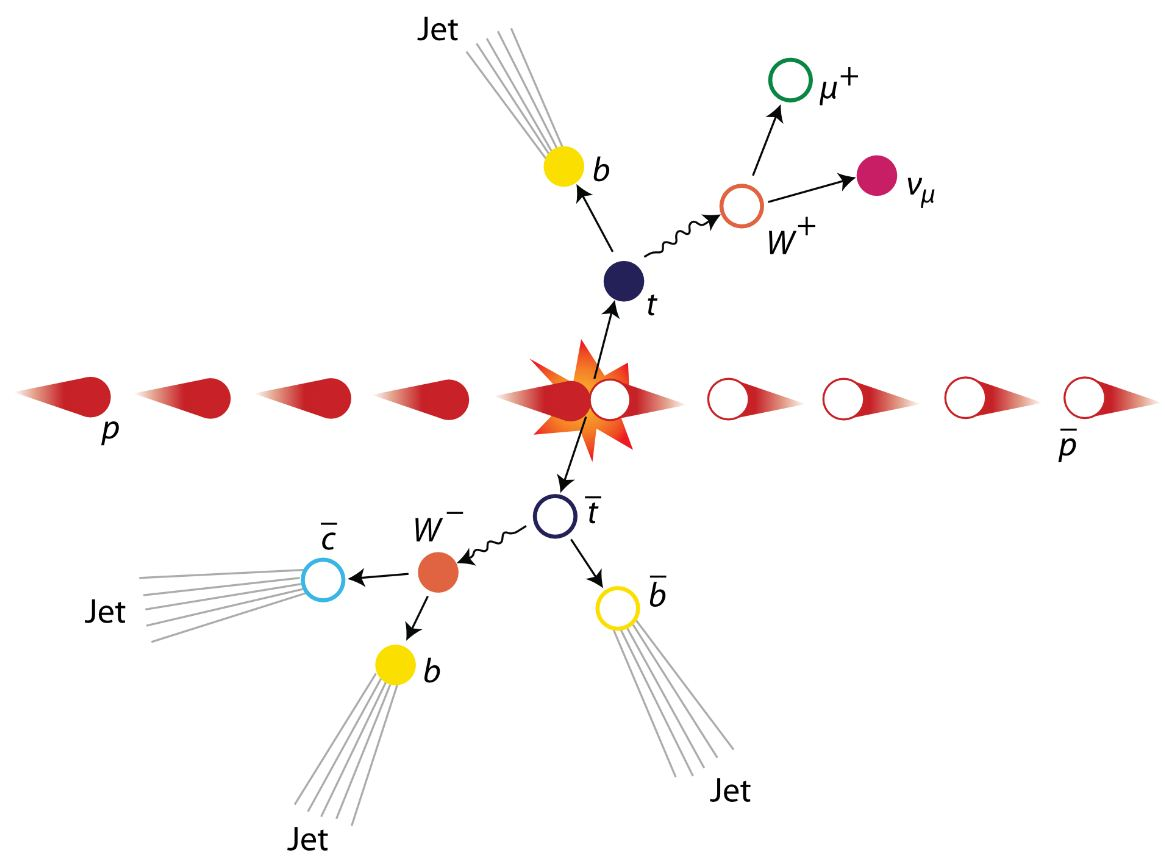
\includegraphics[width=10cm]{figure/collision.JPG}}
\caption[Dos]{ Gr�fico del conteo de fotoelectrones para cada una de las celdas respecto a su distancia a la posici�n incidente de la part�cula (en una de los ejes). Los valores son calculados para un gamma de 10 GeV en incidencia normal. En rojo se muestra la parametrizaci�n de la curva utilizando la ecuaci�n~\ref{eq:lateral}.  \label{fig:lateral}}
\end{figure}


El algoritmo de unfolding comienza con una estimaci�n del conteo de fotoelectrones y posici�n de las lluvias correspondientes a cada m�ximo. Para esto se utilizan los valores de conteo y posici�n central de las celdas correspondientes a los m�ximos locales. Entonces algoritmo continua de acuerdo a lo explicado en la Secci�n~\ref{solapamiento}, adaptado para el caso unidimensional,  con la diferencia que el algoritmo continua si cualquiera de las posiciones estimada para los clusters en uno de los ejes cambia en m�s de 0.01 celdas. En caso que el algoritmo no converga luego de 20 iteraciones el cluster es descartado. 

%El algoritmo completo para el caso unidimensional del detector preshower es resumido en el diagrama de la Figura~\ref{fig:algunfolding}. 

\subsection{Reconstrucci�n de posici�n y energ�a}

Como se mencion� en le Secci�n~\ref{posicion}, la forma m�s simple de reconstruir la posici�n de un part�cula incidente es usando el centro de gravedad, expuesto en la ecuaci�n~\ref{eq:weightedsum}.  Donde $w_i$ en la suma con pesos corresponder�a al conteo de fotoelectrones en cada una de las celdas. Se sabe que esta ecuaci�n produce errores sistem�ticos dependiendo de la posici�n dentro del cristal en la que incide la part�cula, esto debido a la subvaloraci�n de las colas exponenciales en la ecuaci�n. Para observar si esto ocurre para el detector preshower se gr�fica la posici�n incidente $x_{inc}$ versus la posici�n reconstruida $x_{rec}$ media para varias posici�n de incidencia en el cristal central para una part�cula gamma de 10 GeV. Como se observa en la Figura~\ref{fig:curvaS}~a), para el detector preshower existe un error sistem�tico en la reconstrucci�n utilizando el centro de gravedad, la forma S de la curva muestra que las posiciones son reconstruidas err�neamente en las posiciones lejos de los l�mites o lejos del centro del cristal (esto puede ser explicado debido a la cantidad de energ�a que se filtra al resto de los cristales, en el centro la mayor�a de la energ�a esta en el cristal de incidencia, por lo que la posici�n puede ser reconstruida correctamente, mientras que en los l�mites la mayor�a de la energ�a esta en los cristales aleda�os, permitiendo una buena reconstrucci�n tambi�n).

En la Secci�n~\ref{posicion} se present� un m�todo simple para solucionar el problema que presenta la ecuaci�n del centro de gravedad. Este m�todo se basa en la ecuaci�n~\ref{eq:weightedsumexp}, que se encarga autom�ticamente de las colas con forma exponencial de la lluvia electromagn�tica en el detector preshower. Para utilizar esta ecuaci�n es necesario definir el valor $w_0$. Para esto se utilizaron simulaciones. Se midi� el error medio de reconstrucci�n $<x_{rec} - x_{inc}> $ para diferentes valores de $w0$ para gammas incidentes de manera normal y uniformemente distribuidos en el rect�ngulo central de 40x40 mm. Se midieron los valores para gammas de 5, 10 y 15 GeV. En la Figura~\ref{fig:w0error} se muestran los resultados, en base a esto se decidi� utilizar un $w_0 = 3$ que presenta la menor perdida de resoluci�n a diferentes energ�as. En la Figura~\ref{fig:curvaS}~b) se muestra la misma curva S, obtenida anteriormente que gr�fica la posici�n reconstruida versus la posici�n incidente. Se observa que los errores sistem�ticos ahora son mucho menores, solucionando el problema que presenta el centro de gravedad.

\begin{figure}[t]
\makebox[\textwidth][c]{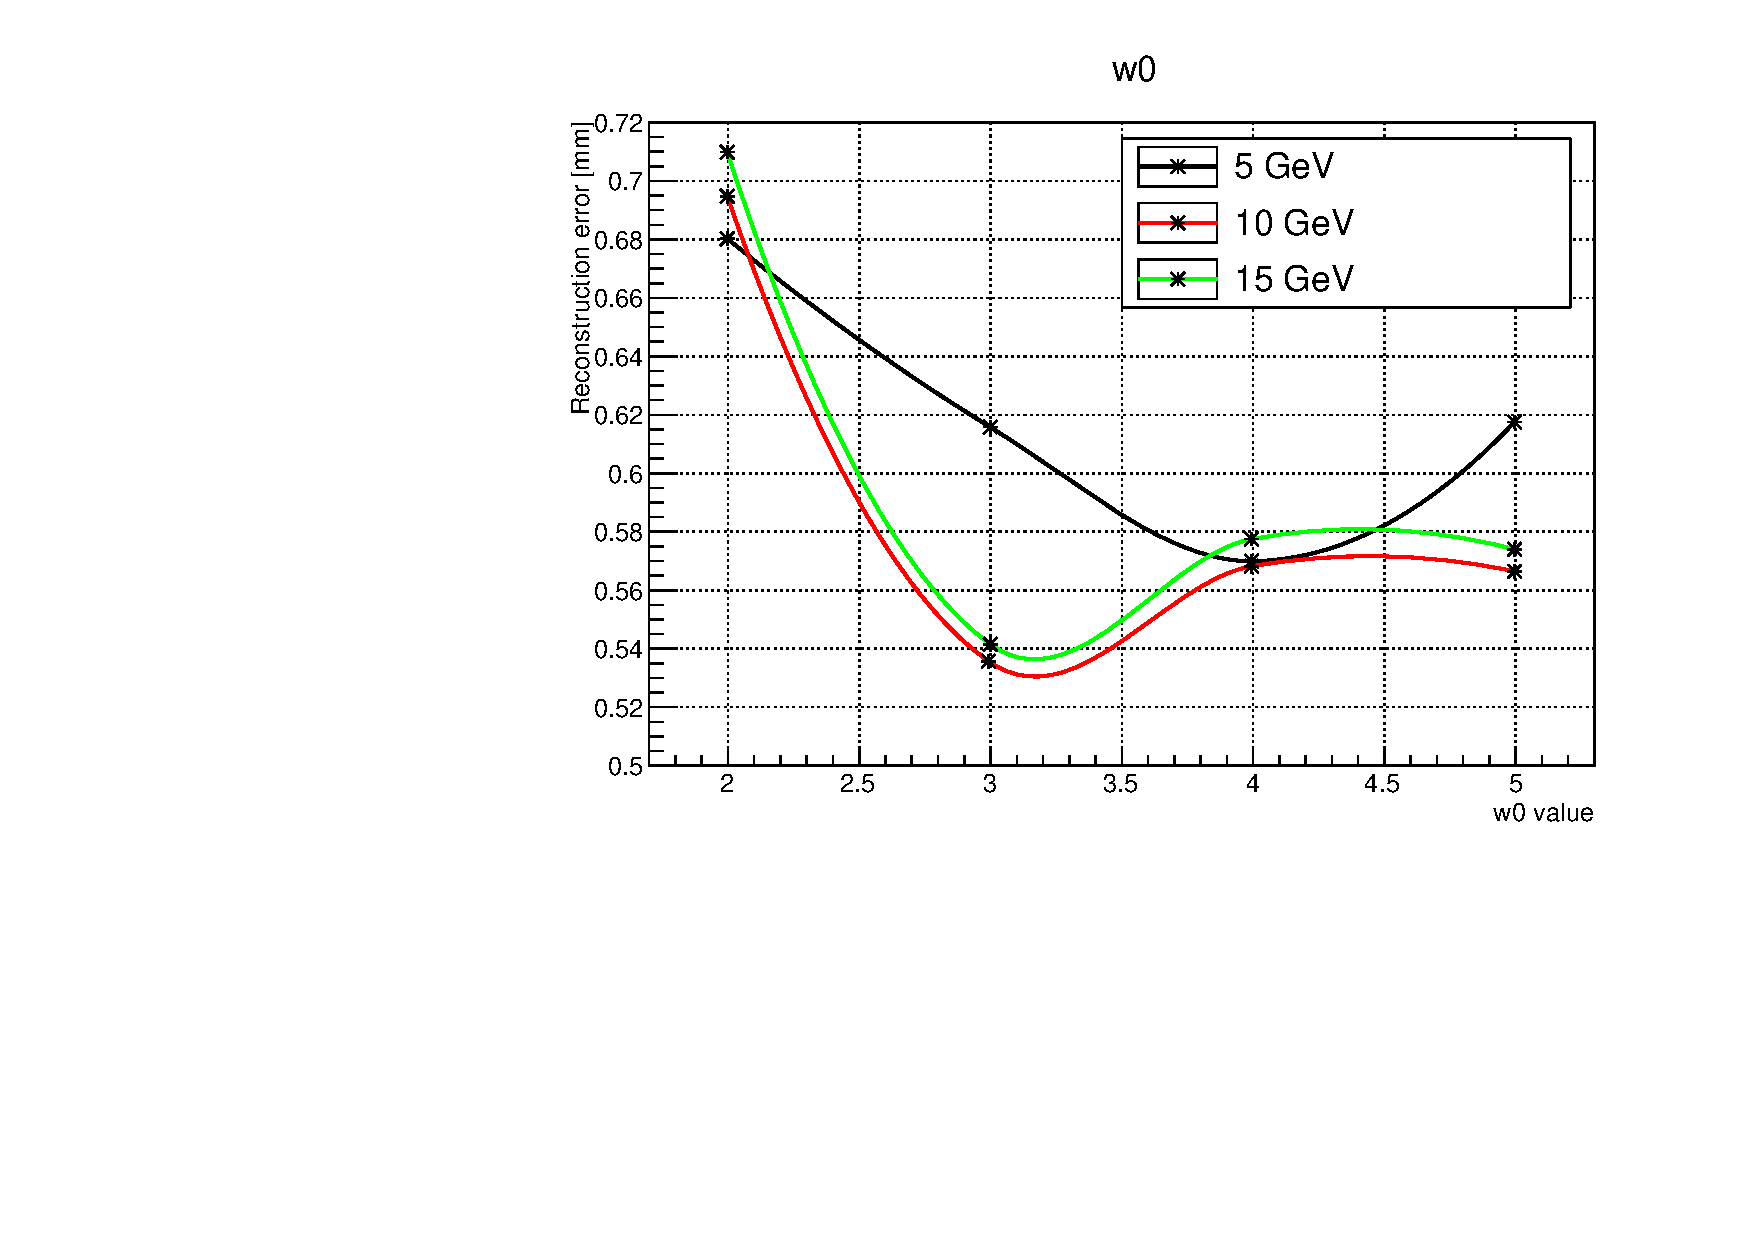
\includegraphics[width=15cm]{figure/w0error.pdf}}
%{\centering 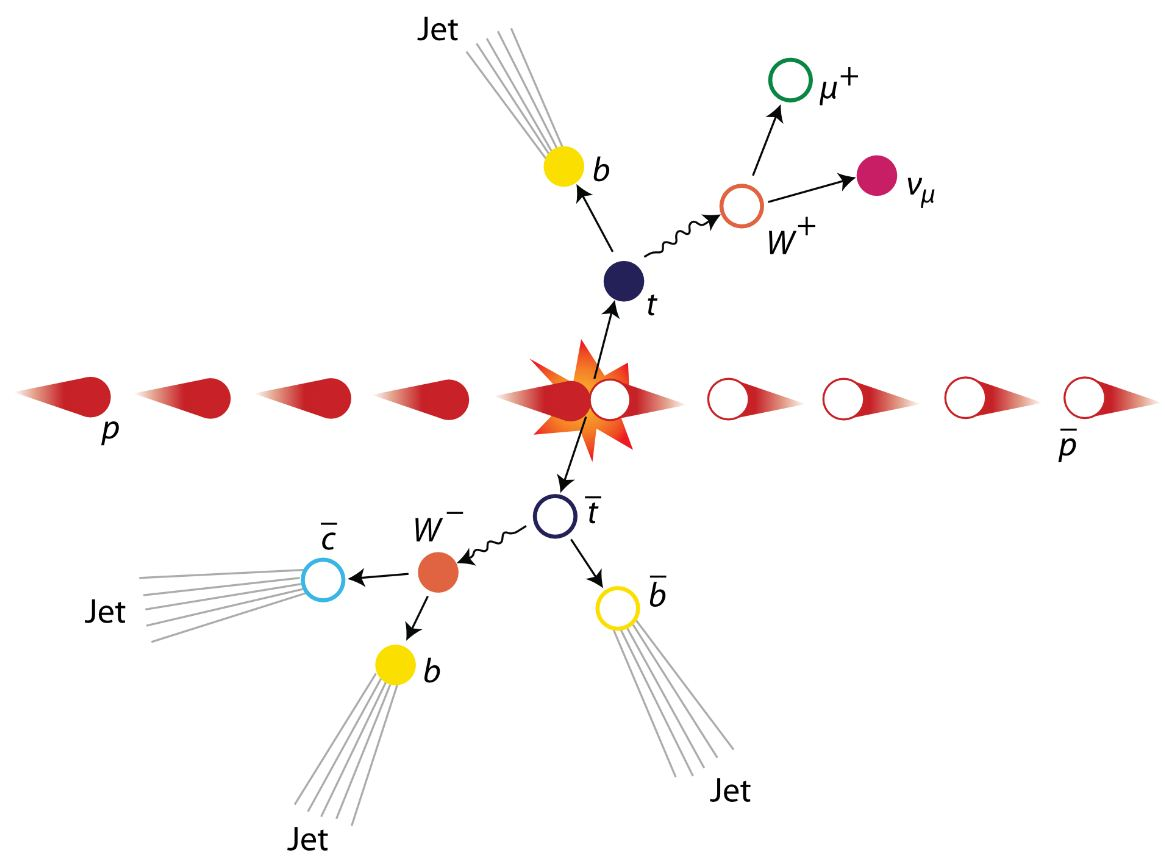
\includegraphics[width=10cm]{figure/collision.JPG}}
\caption[Dos]{ Error de reconstrucci�n versus valor de $w_0$ en~\ref{eq:weightedsumexp} para el m�todo de reconstrucci�n de posici�n \label{fig:w0error}}
\end{figure}


\begin{figure}
    \centering
    \begin{subfigure}[b]{0.9\textwidth}
        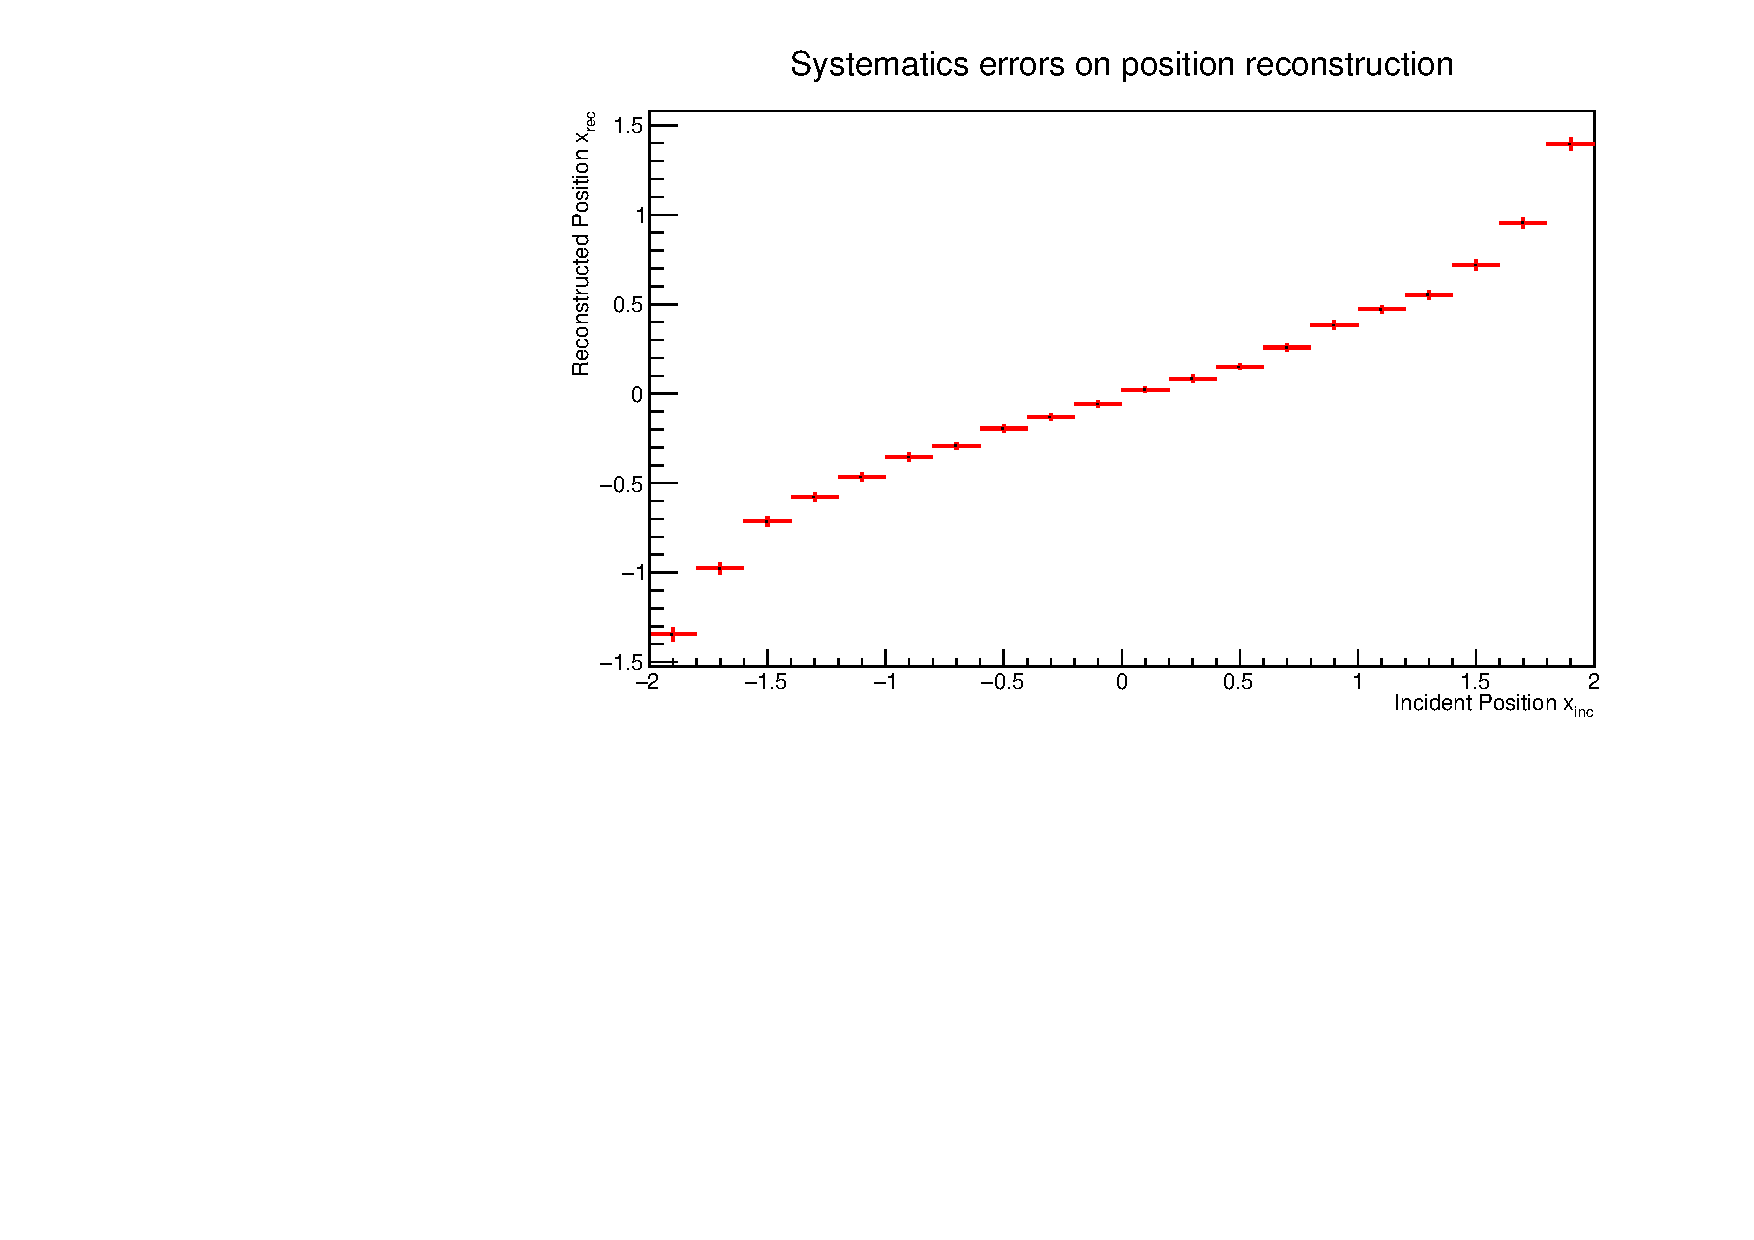
\includegraphics[clip, width=\textwidth]{figure/position_no_w.pdf}
        \caption{Posici�n reconstruida utilizando el m�todo de centro de gravedad. }
    \end{subfigure}
    ~
    \begin{subfigure}[b]{0.9\textwidth}
        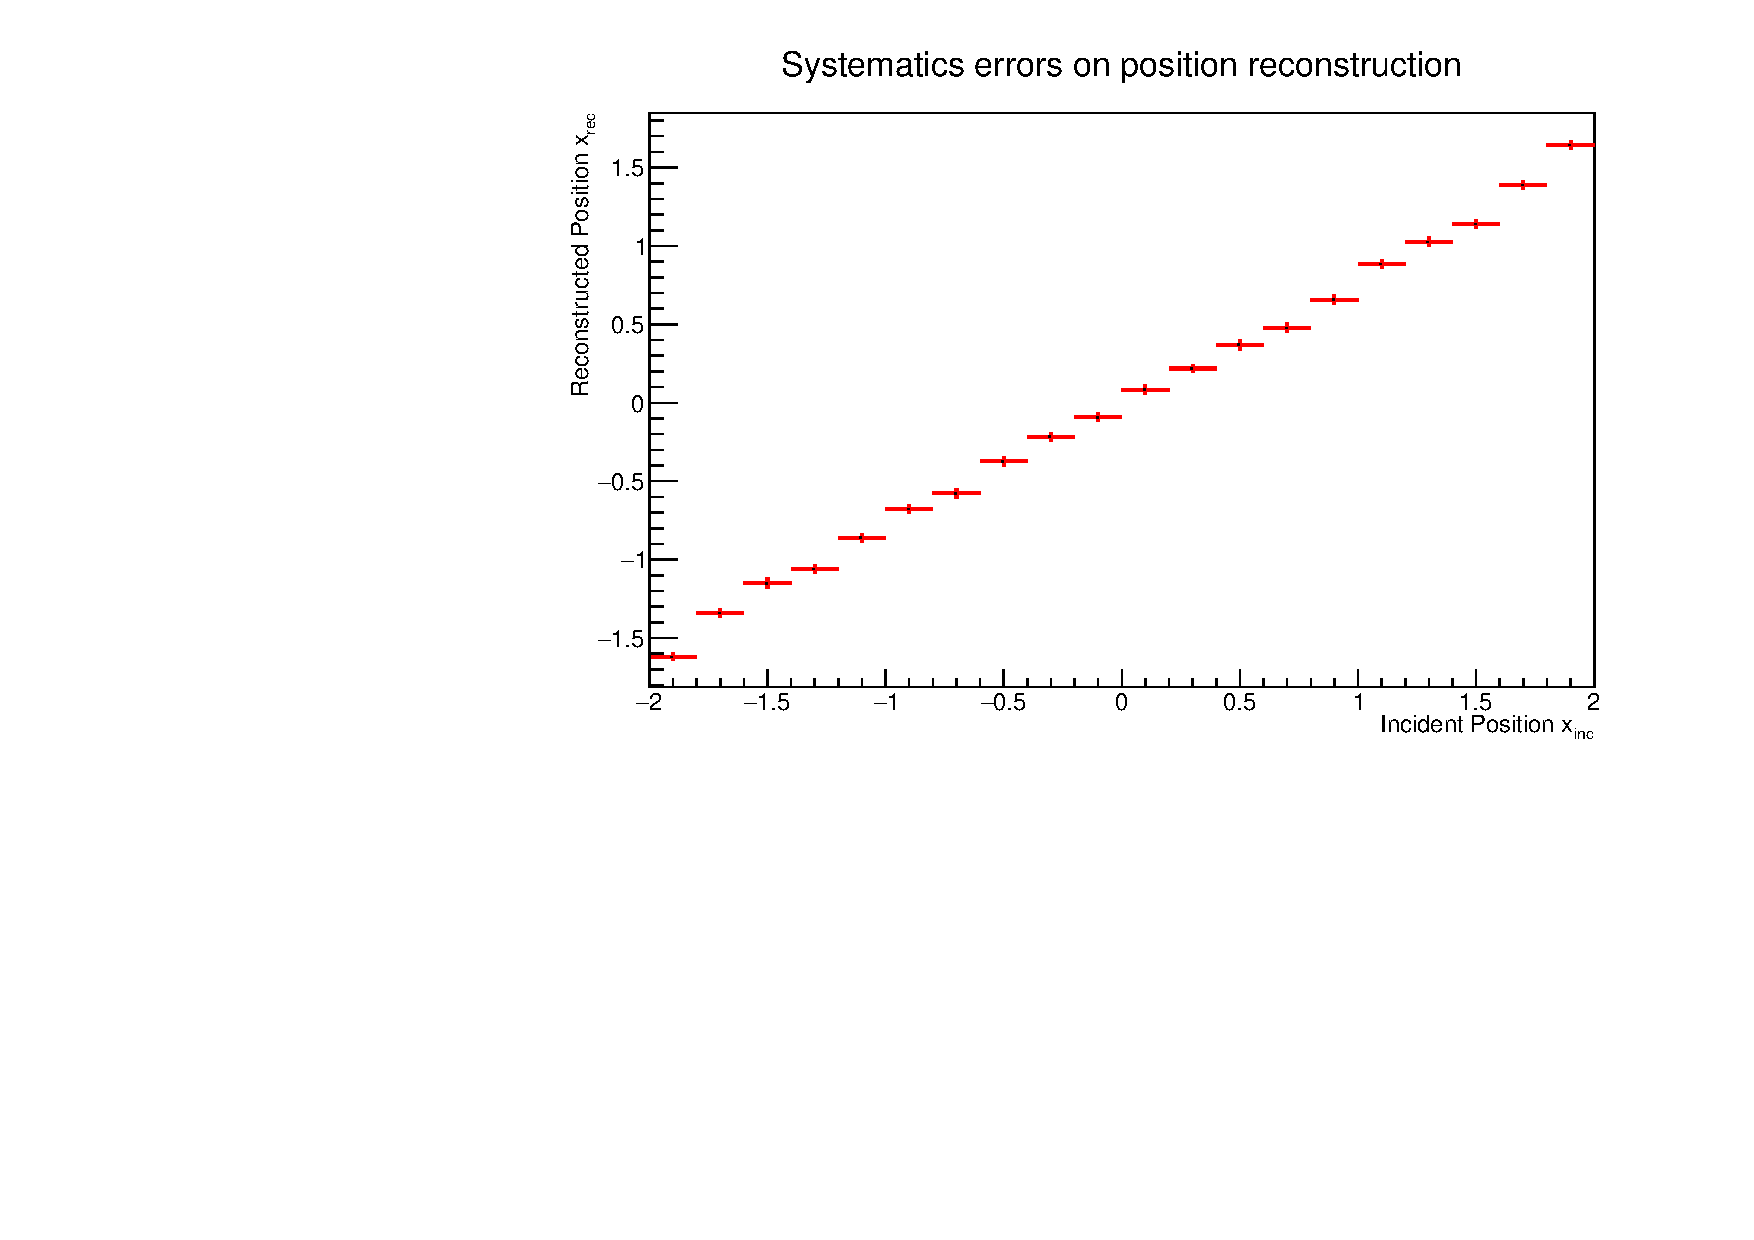
\includegraphics[clip,width=\textwidth]{figure/position_w.pdf}
        \caption{Posici�n reconstruida utilizando la ecuaci�n~\ref{eq:weightedsumexp}. }
    \end{subfigure}

    \caption{Gr�fico de posici�n incidente $x_{inc}$ versus posici�n reconstruida $x_{rec}$ (para uno de los ejes). En el gr�fico se muestran los valores medios para la posici�n reconstruida en varias posiciones de incidencia. El gr�fico permite observar los errores sistem�ticos que se presentan debido a las diferentes posiciones de incidencia dentro de un mismo cristal. }
    \label{fig:curvaS}
\end{figure}

\subsection{Resoluci�n de ambig�edades}
Una gran diferencia entre el sistema de lectura del detector Preshower y los sistemas de lecturas comunes de otros detectores es que la informaci�n del detector preshower es obtenida por dos arreglos de MPPC ubicados en los extremos derecho y superior de la matriz de cristales. Cada uno de estos arreglos de lectores s�lo recibe una proyecci�n de la energ�a en el plano unidimensional, mientras que la posici�n debe ser reconstruida en el plano bidimensional. Esto provoca ciertas ambig�edades que deben ser resueltas si se quiere obtener la posici�n incidente de la part�cula. Tal como se observa en la Figura~\ref{fig:ambig}, este sistema provoca situaciones en las que es dif�cil combinar las posiciones incidentes unidimensionales para reconstruir la posici�n bidimensional. Si, por ejemplo, en uno de los ejes se observa s�lo una part�cula pero en el otro se observan dos, significa que la part�cula aparece solapada en uno de los ejes y la energ�a correspondiente a cada part�cula puede ser identificada en base a la reconstrucci�n del eje en que se observan ambas part�culas. Por otro lado, considerar que en ambos ejes se observan dos part�culas, entonces no es claro que posici�n en uno de los ejes corresponde a que posici�n en el otro eje, es decir, s�lo considerando la informaci�n de posici�n, es imposible decir si es que la reconstrucci�n debiese ser (X1, Y1) y (X2, Y2) o (X1, Y2) y (X2, Y1). 

El problema se complica m�s a�n cuando m�s de dos part�culas inciden, en tales casos las combinaciones posibles crecen factorialmente con el n�mero de part�culas observadas en los ejes ($\mathcal{O}((N_x + N_y)!)$).

Ahora, es posible solucionar este problema considerando el conteo de fotoelectrones reconstruidos para cada part�cula en cada eje. Debido a que el valor medido en cada eje es una proyecci�n de la suma de conteos de los cristales por los que pasa la fibra que llega al lector, entonces, clusters con energ�as similares (no iguales, ya que existe algo de perdida en la propagaci�n) en distintos ejes corresponder�n a la misma part�cula. Para esto debemos asumir, primero, que las perdidas en la propagaci�n de fotones de los cristales a las fibras es despreciable con respecto a la energ�a depositada por la part�cula y segundo que dos part�culas no depositar�n exactamente la misma energ�a. Debido a que la interacci�n de la part�cula con el material en el detector preshower es un proceso probabil�stico, es muy poco probable que dos part�culas interact�en en la misma posici�n y por consiguiente depositen la misma energ�a.  Basado en esto es posible resolver las ambig�edades en la reconstrucci�n mediante la uni�n de clusters con energ�as parecidas en los distintos ejes. 

Para el caso m�s simple, en el que dos part�culas inciden en el detector preshower un algoritmo de resoluci�n de ambig�edades en presentado en Algoritmo~\ref{alg:resolucion}.

\begin{algorithm}
\caption{Resoluci�n de ambig�edades}
\label{alg:resolucion}
\begin{algorithmic}[1]
\State{$X, E_x \leftarrow$ Reconstruction1D(X)}
\State{$Y, E_y \leftarrow$ Reconstruction1D(Y)}
\If{$len(X) > 1$ and $len(Y) > 1$}
	\State{$D_0 = | E_x[0] - E_y[0] |$}
	\State{$D_1 = | E_x[0] - E_y[1] |$}
	\If{$D_0 < D_1$}
		\State{$P_0 = (X[0], Y[0])$}
		\State{$P_1 = (X[1], Y[1])$}
		\State{$E_0, E_1 = E_x[0], E_x[1]$}
	\Else{}
		\State{$P_0 = (X[0], Y[1])$}
		\State{$P_1 = (X[1], Y[0])$}
		\State{$E_0, E_1 = E_x[0], E_x[1]$}
	\EndIf
\ElsIf{$(len(X) > 1$ and $len(Y) == 1)$ } \Comment{Similar para el caso opuesto.}
	\State{$P_0 = (X[0], Y[0])$}
	\State{$P_1 = (X[1], Y[0])$}
	\State{$E_0, E_1 = E_x[0], E_x[1]$}
\ElsIf{$(len(X) == 1$ and $len(Y) == 1)$ } 
	\State{$P_0 = (X[0], Y[0])$}
	\State{$E_0, E_1 = E_x[0], E_x[1]$}
\EndIf
\end{algorithmic}
\end{algorithm}

Este caso es el m�s com�n e importante de identificar, ya que es el producido por el decaimiento de un pi�n neutro. Sin embargo el problema se puede complicar considerablemente m�s cuando m�s de dos part�culas son identificadas en alguno de los ejes (varias combinaciones entre una, dos o m�s de dos part�culas son posibles). Si el n�mero de part�culas es muy grande es muy costoso computacionalmente considerar todas las posibilidades, por lo que un algoritmo heur�stico que permita encontrar la combinaci�n m�s probable de part�culas basado en el conteo de fotoelectrones de cada cluster ser�a una buena opci�n a considerar. Para esto se necesita estudiar y proponer un nuevo algoritmo para la tarea de resoluci�n de ambig�edades, lo que queda fuera del alcance de este trabajo.

\section{An�lisis de resultados} 
En esta secci�n se presentar�n los resultados del algoritmo presentado. Se debe notar que el prop�sito principal del detector preshower es identificar part�culas muy cercanas entre s�. La reconstrucci�n de posici�n y de energ�a son un trabajo conjunto de todas las secciones del detector. Si bien la reconstrucci�n de posici�n se puede realizar con el detector preshower, un trabajo m�s preciso puede ser realizado por otro tipos de detectores especializados para la tarea. Por otro lado, la reconstrucci�n de energ�a es un trabajo realizado por otro tipos de detectores en la cadena de detecci�n y no es proposito del detector preshower. El detector presentado aqu� s�lo es capaz de medir el conteo de fotoelectrones que se comporta como una distribuci�n de Poisson con media relacionada a la energ�a detectada. En base a lo anteriormente dicho los resultados presentados en esta secci�n se concentrar�n en evaluar la capacidad del detector para la separaci�n de part�culas cercanas y su capacidad para reconstruir su posici�n. Otros resultados pueden ser encontrados en el Ap�ndice~\ref{ApendiceB}. 

Los resultados presentados en esta secci�n se obtuvieron mediante simulaciones en el rango 1-15GeV. Se utilizaron 5000 pares de part�culas gamas lanzadas en posiciones de incidencia uniformemente distribuidas en el cuadrado de 40x40 mm central de la matriz de cristales y con �ngulo de incidencia perpendicular a la cara frontal del detector preshower. No se presentan experimentos con �ngulos de incidencia no perpendicular y estos casos se analizar�n con m�s profundidad en las conclusiones.

\subsection{Identificaci�n de part�culas cercanas}

La Figura~\ref{fig:clusters} muestra para diferentes combinaciones de part�culas de distintas energ�as a que distancia (entre las part�culas) dos part�culas pueden ser identificadas por el detector. Se observa que clusters con un s�lo m�ximo (cuando dos part�culas son imposibles de detectar) son observados principalmente a distancias peque�as entre las dos part�culas ($\leq 5$ unidades de celda, es decir $\leq 20$ mm). Por otro lado, clusters con dos m�ximos que deben ser separados mediante el procedimiento de unfolding se observan entre las 5 y 20 unidades de celda (25-100 mm). Los clusters totalmente separados se observan en poca cantidad y principalmente sobre la distancia de 15 unidades de celdas  (75 mm). Tambi�n se observa que existe un l�mite claro para la resoluci�n de dos part�culas del detector preshower, el que es 5 unidades de celda (o 20 mm).

\begin{figure}
    \centering
    \begin{subfigure}[b]{0.48\textwidth}
        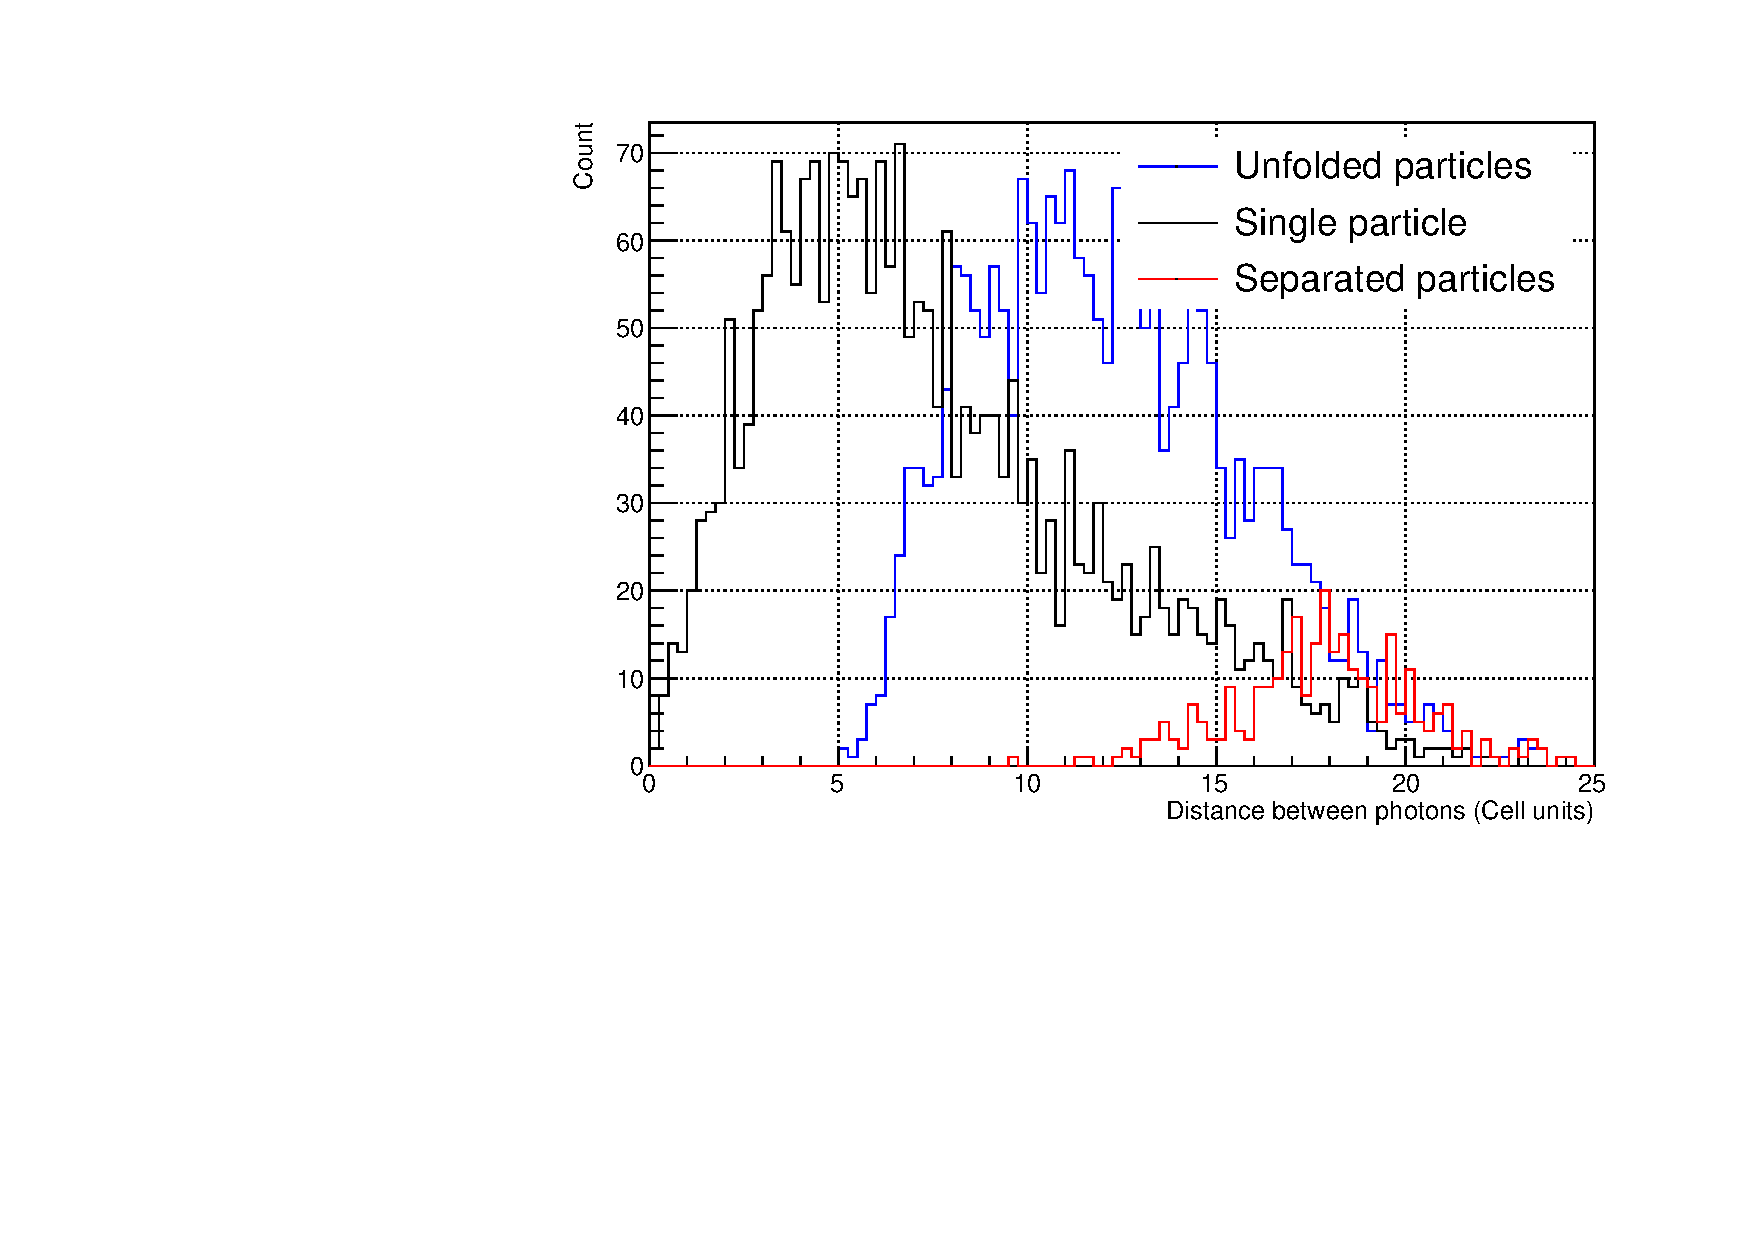
\includegraphics[clip, width=\textwidth]{figure/10_1/2D_clusters.pdf}
        \caption{10 + 1 GeV. }
    \end{subfigure}
    ~
    \begin{subfigure}[b]{0.48\textwidth}
        \includegraphics[clip,width=\textwidth]{figure/10_5/2D_clusters.pdf}
        \caption{10 + 5 GeV. }
    \end{subfigure}\\
    ~
    \begin{subfigure}[b]{0.48\textwidth}
        \includegraphics[clip, width=\textwidth]{figure/10_10/2D_clusters.pdf}
        \caption{10 + 10 GeV. }
    \end{subfigure}
    ~
    \begin{subfigure}[b]{0.48\textwidth}
        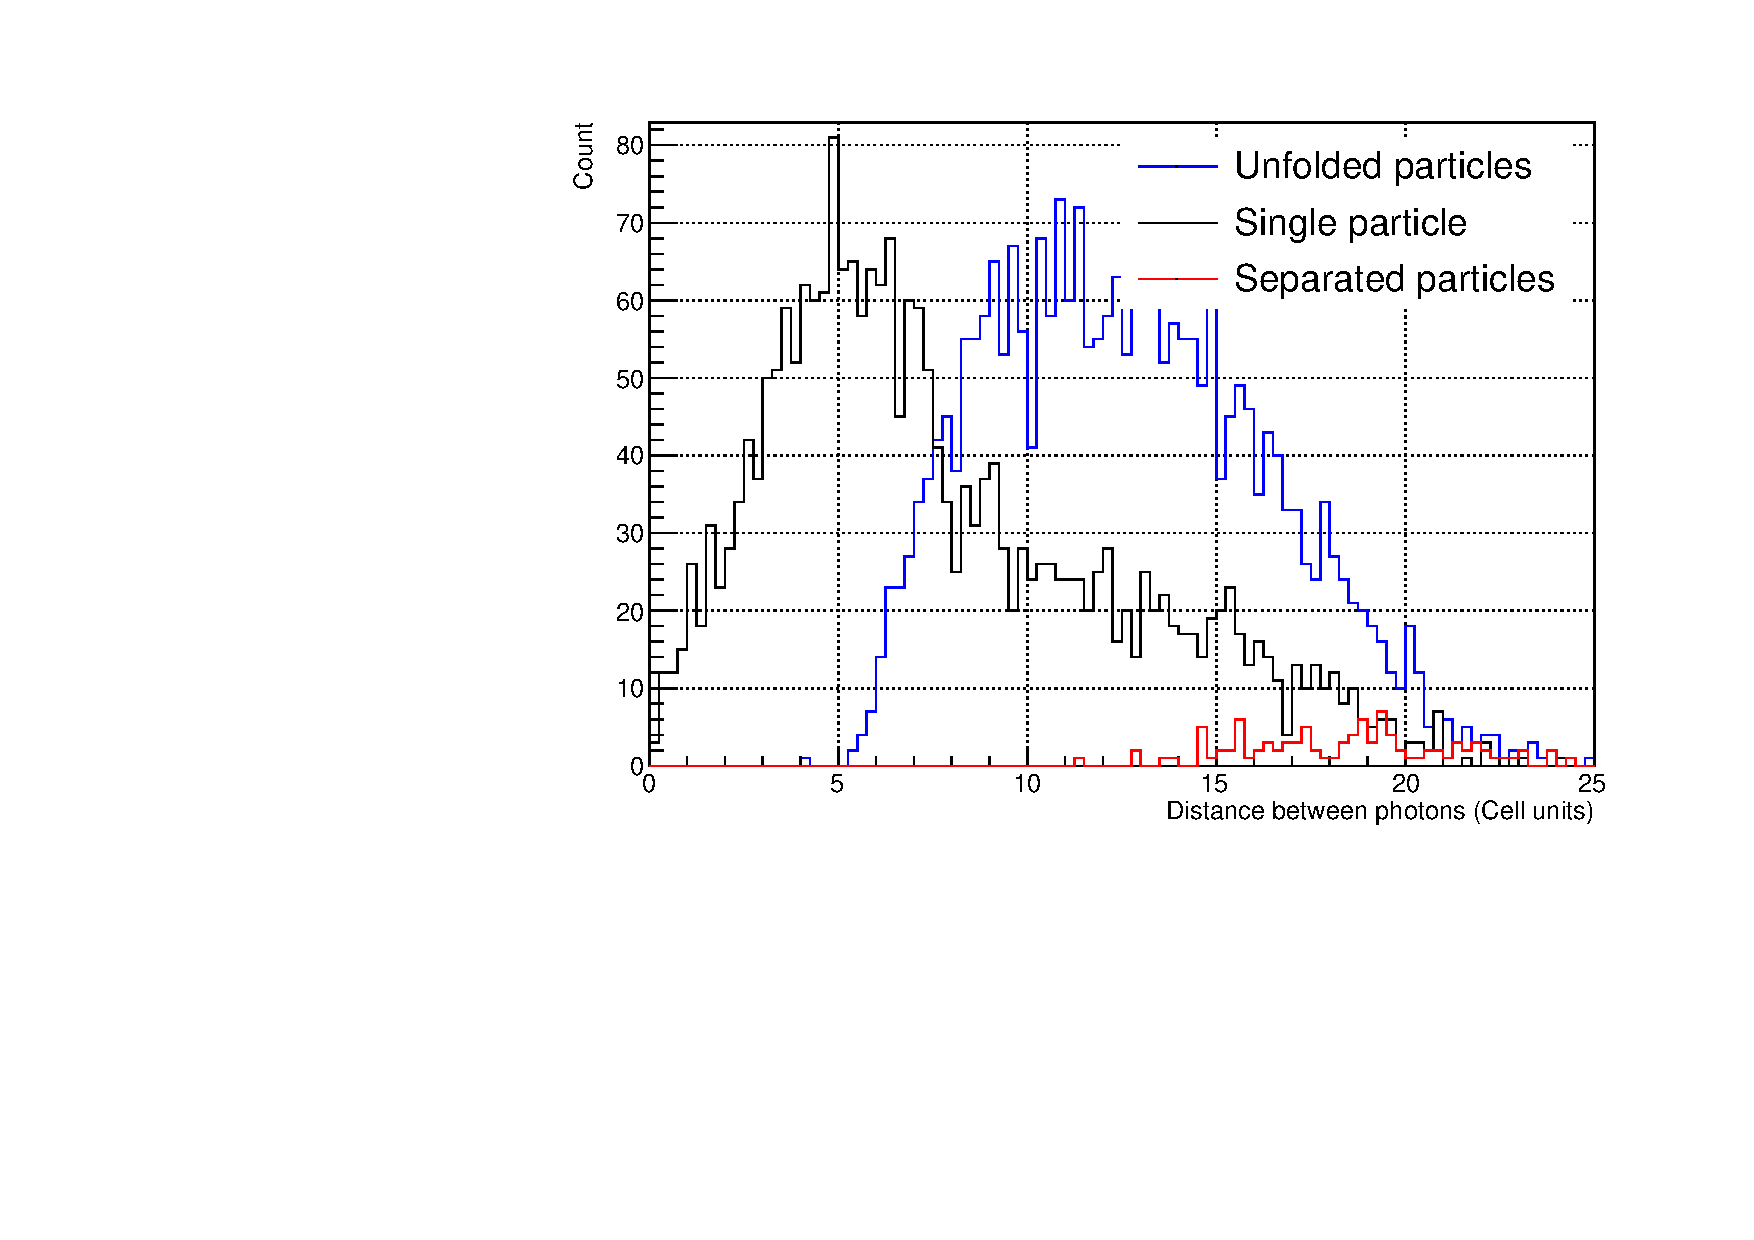
\includegraphics[clip,width=\textwidth]{figure/10_15/2D_clusters.pdf}
        \caption{10 + 15 GeV. }
    \end{subfigure} 
    \caption{N�mero de clusters identificables como una funci�n de la distancia entre las part�culas incidentes. Se analizaron 4 casos (a) 10 GeV + 1 GeV $\gamma$, (b) 10 GeV + 5 GeV $\gamma$, (c) 10 GeV + 10 GeV $\gamma$, (d) 10 GeV + 15 GeV $\gamma$. Para cada uno de los casos se muestran los clusters con s�lo un m�ximo, con dos m�ximos y los clusters totalmente separados.   }
    \label{fig:clusters}
\end{figure}

\subsection{Reconstrucci�n de posici�n}
Para estudiar la eficacia del algoritmo para reconstruir la posici�n de las part�culas incidentes se observ� el error de reconstrucci�n medio entre la posici�n reconstruida por el algoritmo de reconstrucci�n y la posici�n de incidencia de la part�acula ($<X_{rec} - X_{inc}$>). Esto para pares de part�culas de 10 GeV + 1 GeV, 10 GeV + 5 GeV, 10 GeV + 10 GeV , 10 GeV + 15 GeV. Se estudi� el error de reconstrucci�n en los casos en que el algoritmo de unfolding deba ser aplicado y en los casos en que ambas part�culas forman dos clusters separados (el caso de un s�lo m�ximo no se consider�). En la Figura~\ref{fig:reconstruccion} se muestran histogramas para el error de reconstrucci�n para cada uno de los casos mencionados anteriormente. Mientras que en el Cuadro~\ref{tab:resolucion} se resumen los valores para cada uno de los casos. 

\begin{table}[h]
\centering
\begin{tabular}{|p{1.5cm} p{1cm}| p{3cm} p{3cm} p{3cm}  |}
\hline
    &  & \multicolumn{3}{c|}{Resoluci�n posici�n [mm]} \\
\multicolumn{2}{|c|}{Energias  [GeV]} & Unfolded & Separados & Total \\ \hline
\multirow{2}{*}{10 + 1} & 10  & 1.416 $\pm$ 1.102 & 1.075 $\pm$ 0.7435 & 1.3777 $\pm$ 1.0731 \\ 
 & 1  & 1.789 $\pm$ 1.45  & 1.025 $\pm$ 0.6956 & 1.7032 $\pm$ 1.4067 \\ \hline
 \multirow{2}{*}{10 + 5} & 10  & 1.562 $\pm$ 1.189 & 1.183 $\pm$ 1.122 & 1.54 $\pm$ 1.1885 \\ 
 & 5  & 1.683 $\pm$ 1.26 & 1.144 $\pm$ 0.7378 & 1.6517 $\pm$ 1.2421 \\ \hline
 10 + 10 & 10  & 1.571 $\pm$ 1.21 & 1.088 $\pm$ 0.8137 & 1.5532 $\pm$ 1.2011 \\ \hline
 \multirow{2}{*}{10 + 15} & 10  & 1.623 $\pm$ 1.302 & 1.413 $\pm$ 1.012 & 1.6157 $\pm$ 1.2936 \\ 
 & 15  & 1.556 $\pm$ 1.184 & 1.109 $\pm$ 0.815 & 1.5406 $\pm$ 1.1760 \\ \hline
\end{tabular}
\caption{Error de reconstrucci�n para part�culas $\gamma$ solapadas y totalmente separadas. Se presentan resultados para part�culas de 1, 5,10 y 15 GeV.  \label{tab:resolucion}}
\end{table}

Se observa que hay una peque�a dependencia entre el error de reconstrucci�n y la energ�a de la part�cula incidente. Existe una mejora menor cuando la part�cula tiene mayor energ�a, esto es claro en el caso 10+1 donde el error para la part�cula de 1 GeV es claramente mayor que para la part�cula de 10 GeV. Esto se debe a que la lluvia de la part�cula de 10 GeV cubre a la de 1 GeV dificultando la reconstrucci�n de posici�n. Sin embargo, las diferencias entre los errores de reconstrucci�n para el rango 1-15 GeV son relativamente peque�as, lo que muestra la dependencia menor del algoritmo de reconstrucci�n de posici�n con la energ�a de la part�cula incidente. La error de reconstrucci�n es similar para el caso de clusters separados y clusters solapados donde el algoritmo de unfolding debe ser utilizado, esto demuestra la capacidad del algoritmo de unfolding para separar part�culas cercanas. Existe una peque�a diferencia entre ambos errores, lo que es de esperar ya que el algoritmo de unfolding agrega un paso extra de estimaci�n, adem�s que el cubrimiento mutuo de las lluvias electromagn�ticas dificultan la reconstrucci�n de posici�n.

La precisi�n de la reconstrucci�n es muy buena en comparaci�n con otros detectores, esto se profundizar� en la secci�n de conclusiones.

Para un an�lisis m�s detallado de los errores de reconstrucci�n para las distintas situaciones que se presentan en el algoritmo de reconstrucci�n el lector puede dirigirse al Ap�ndice B.

\begin{figure}
    \centering
    \begin{subfigure}[b]{0.48\textwidth}
        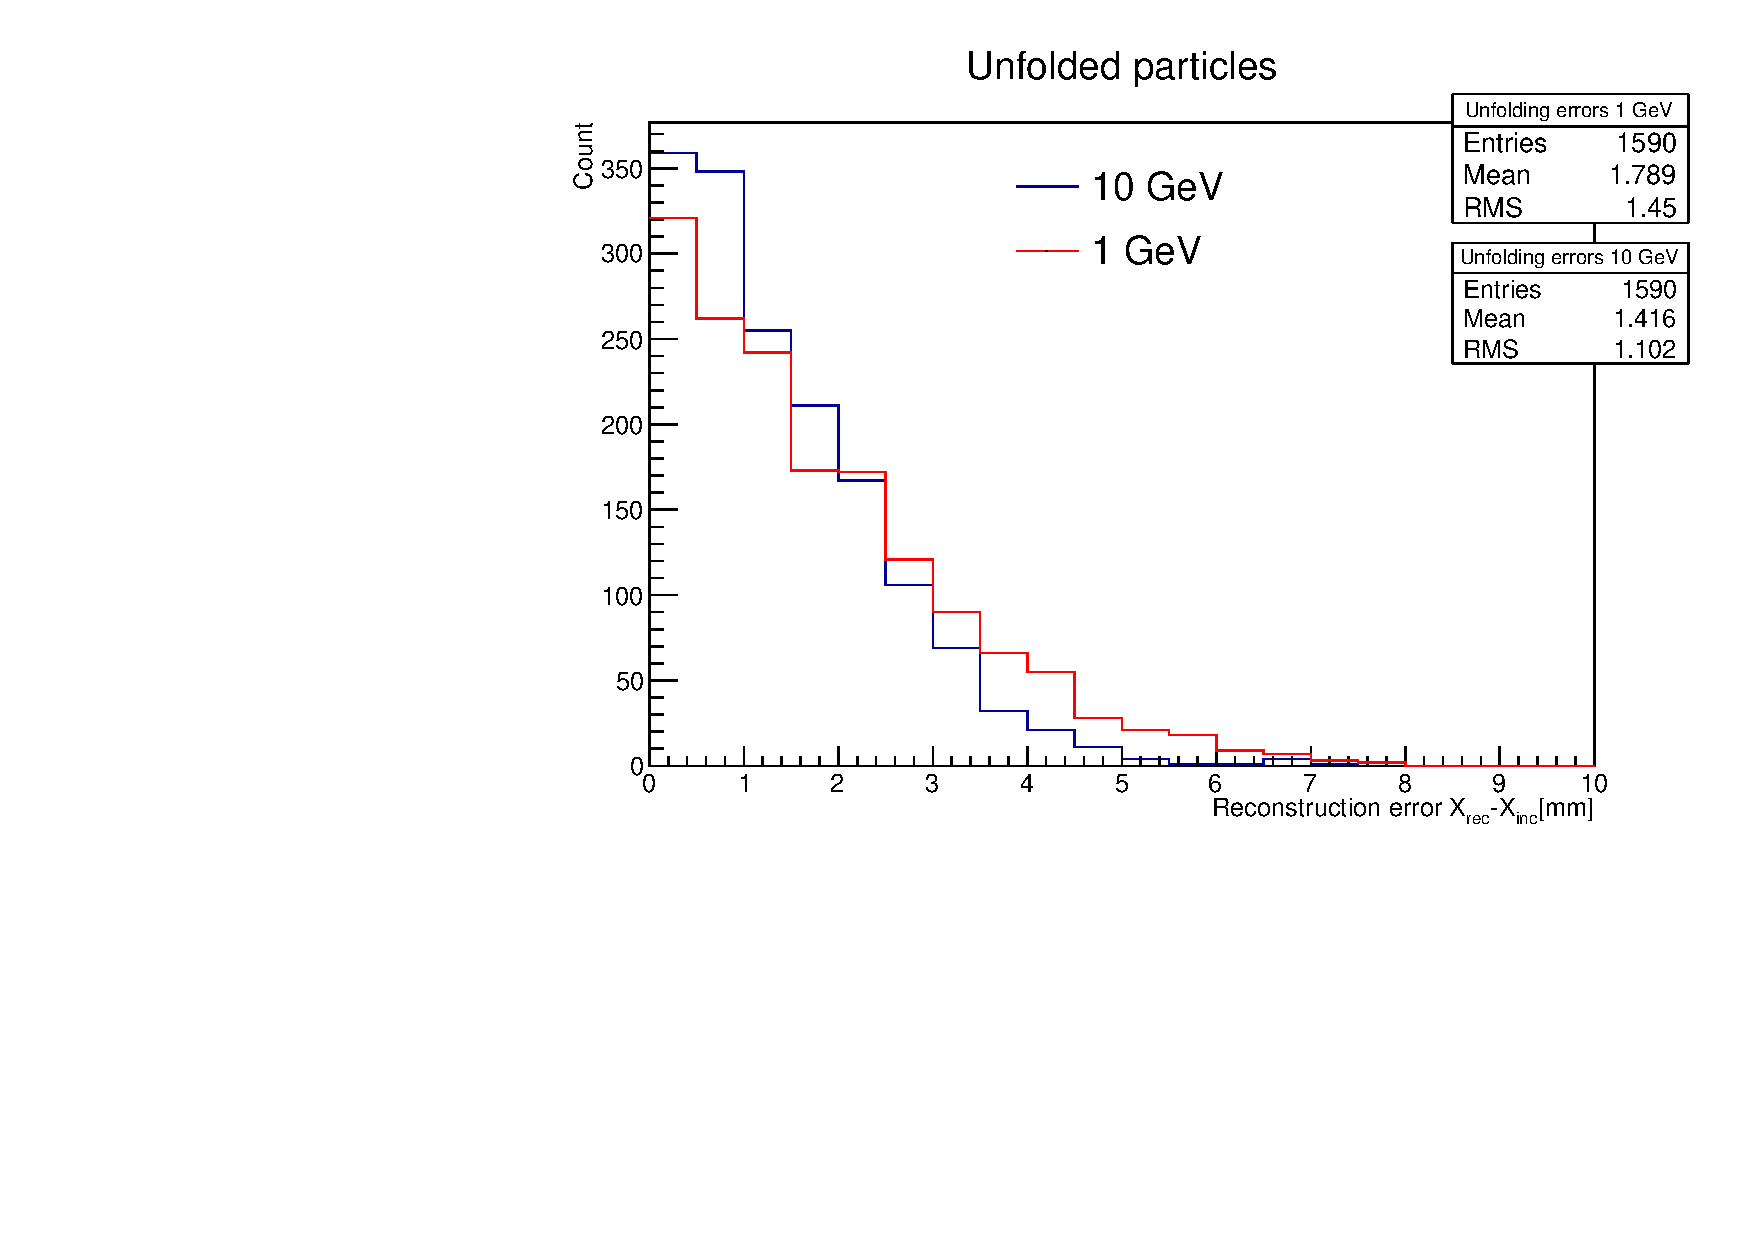
\includegraphics[clip, width=\textwidth]{figure/10_1/x_axis_small_1.pdf}
        \caption{10 + 1 GeV. }
    \end{subfigure}
    ~
    \begin{subfigure}[b]{0.48\textwidth}
        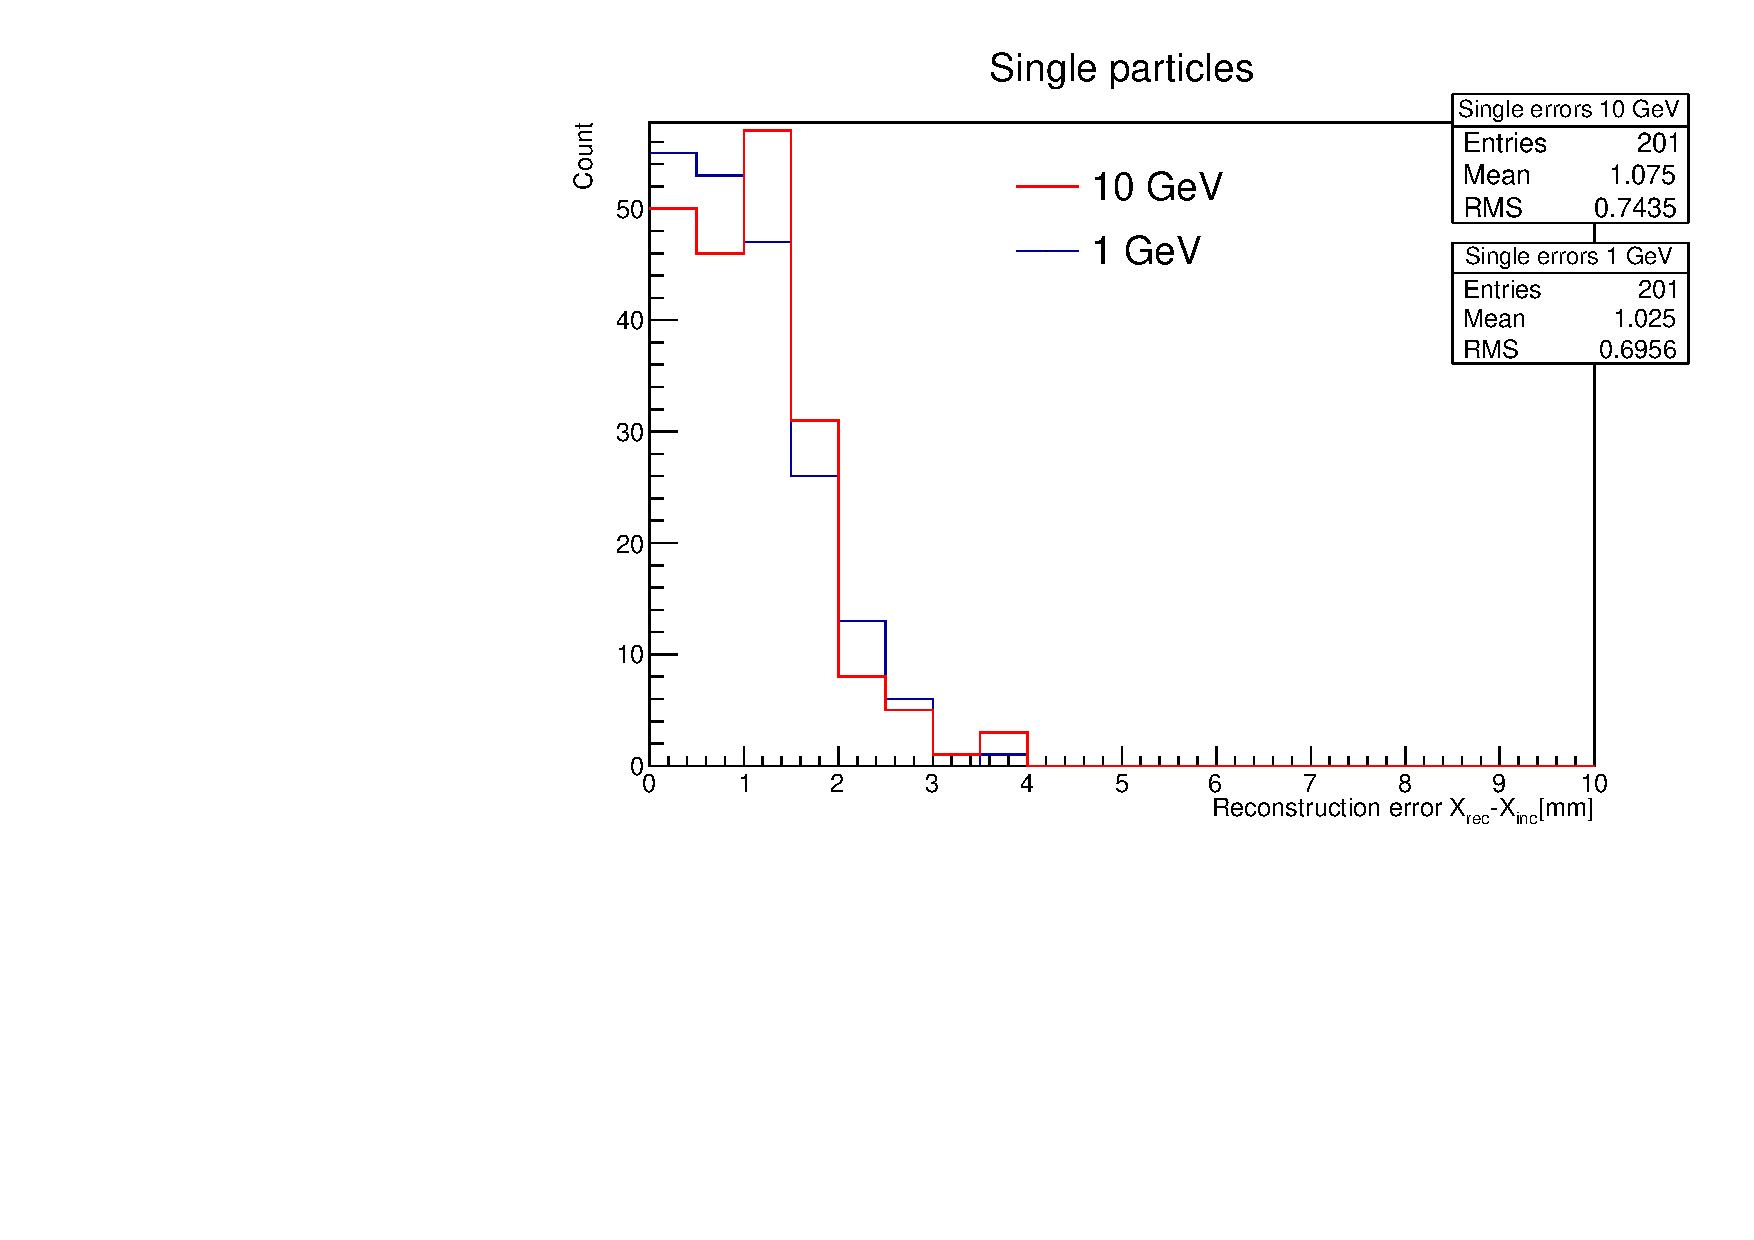
\includegraphics[clip,width=\textwidth]{figure/10_1/x_axis_small_2.pdf}
        \caption{10 + 1 GeV. }
    \end{subfigure}
    ~
    \begin{subfigure}[b]{0.48\textwidth}
        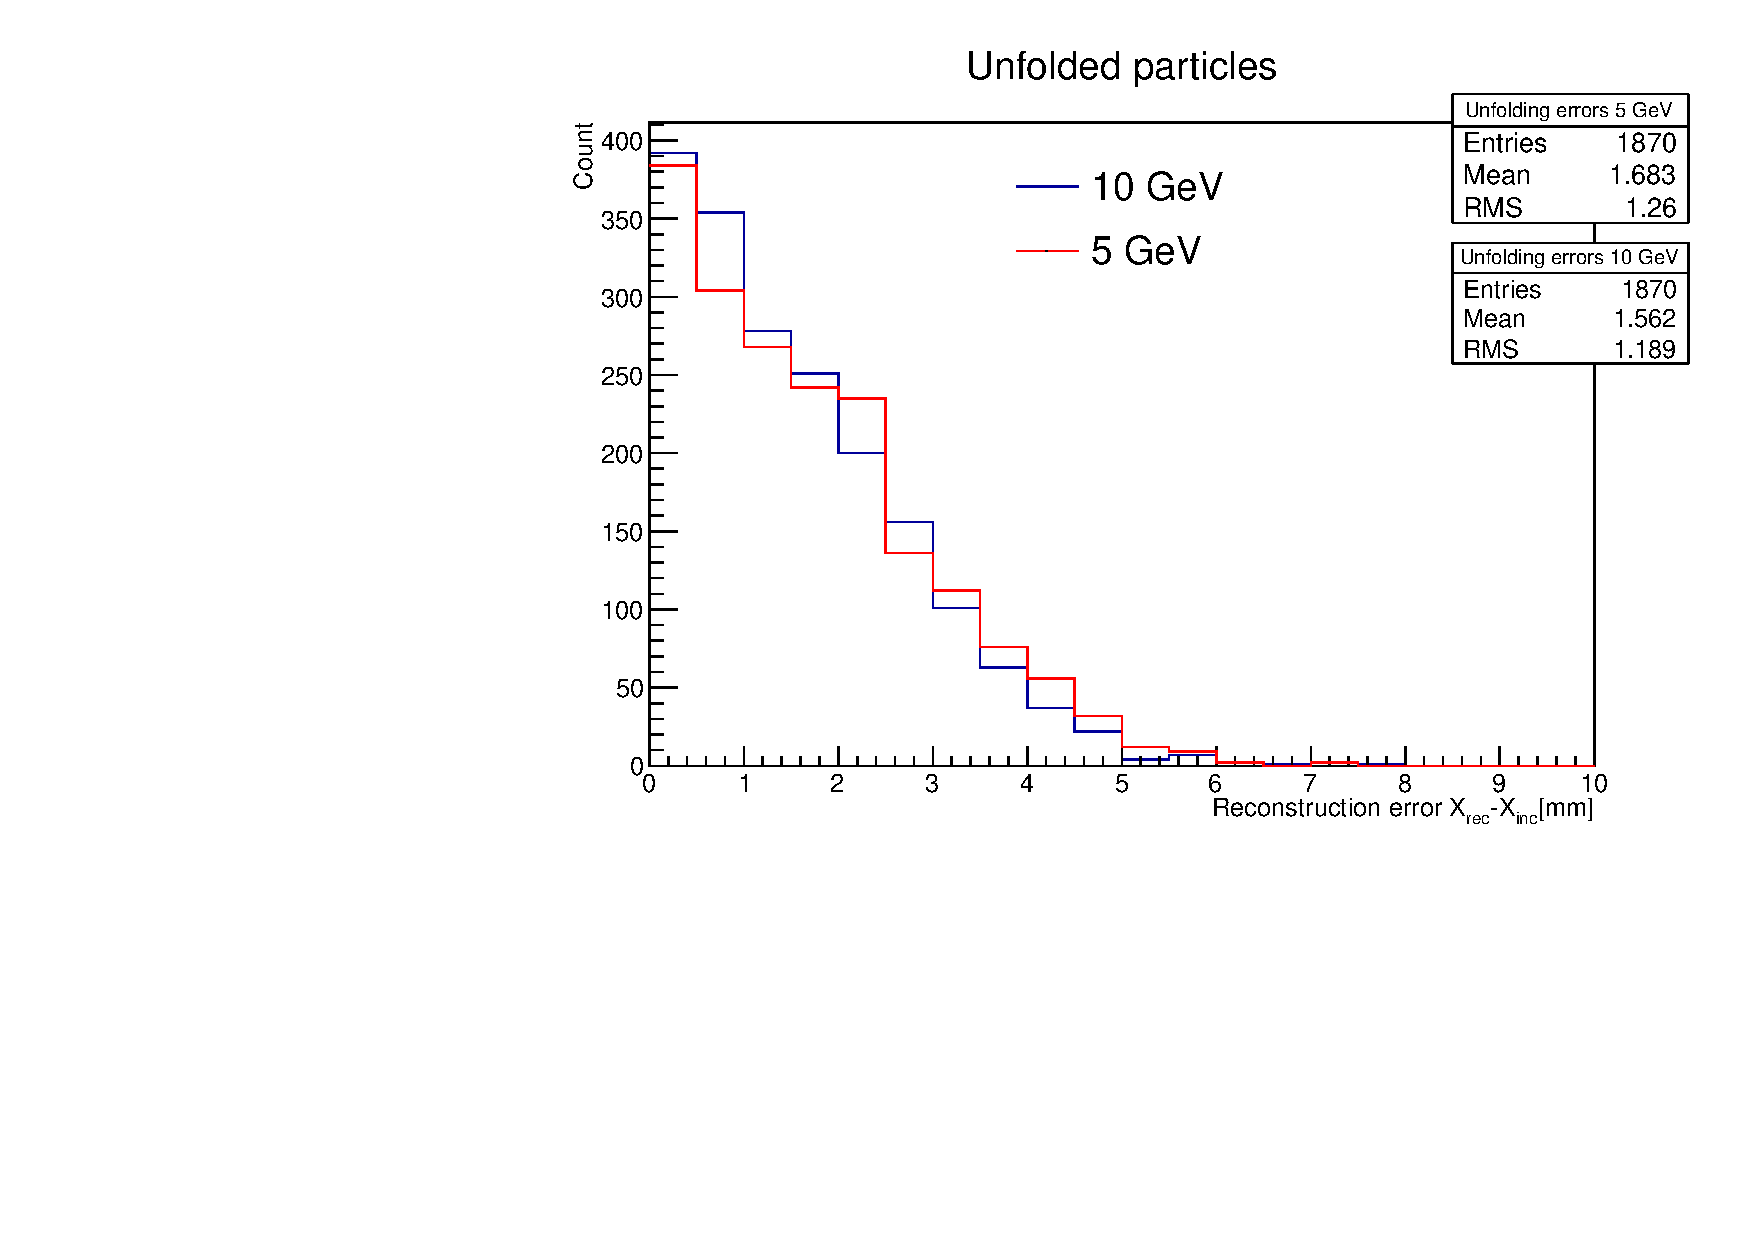
\includegraphics[clip, width=\textwidth]{figure/10_5/x_axis_small_1.pdf}
        \caption{10 + 5 GeV. }
    \end{subfigure}
    ~
    \begin{subfigure}[b]{0.48\textwidth}
        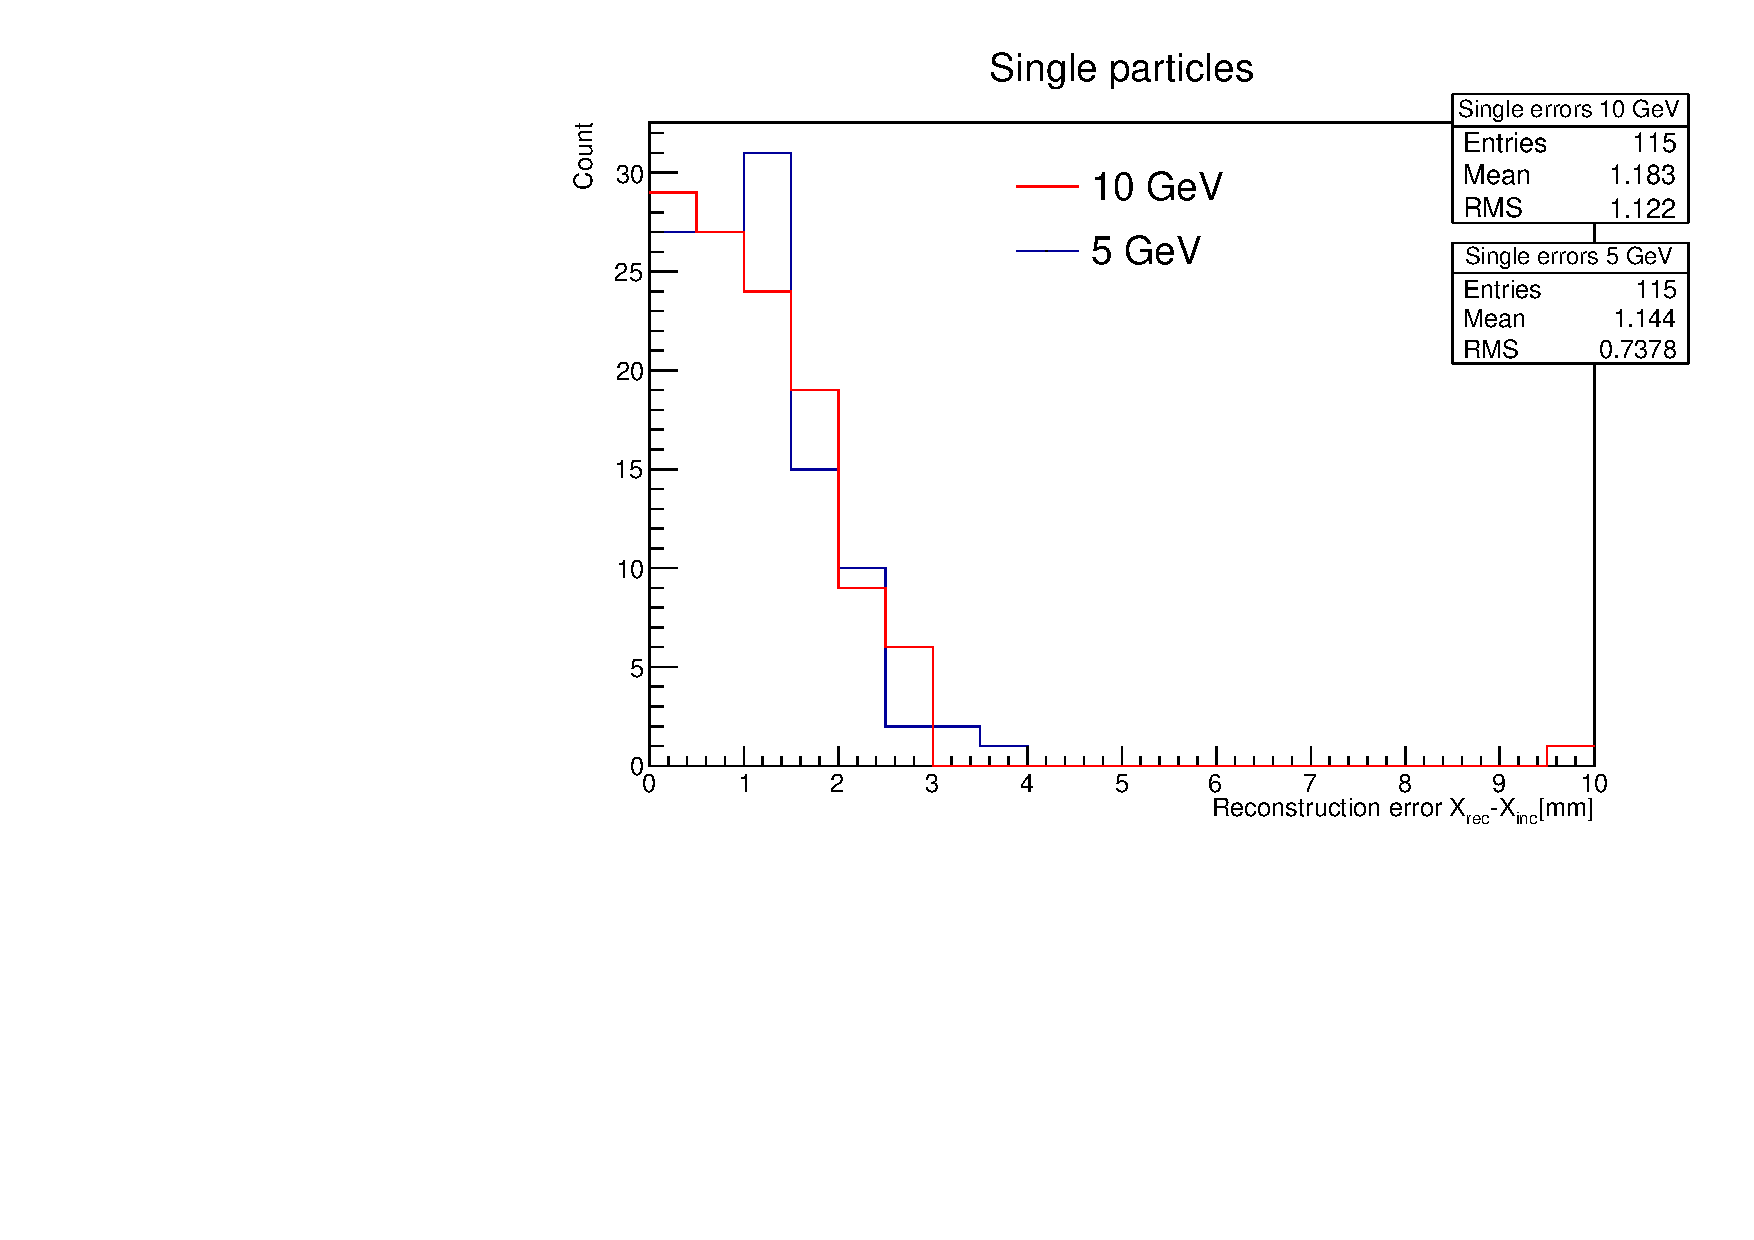
\includegraphics[clip,width=\textwidth]{figure/10_5/x_axis_small_2.pdf}
        \caption{10 + 5 GeV. }
    \end{subfigure}
    ~
    \begin{subfigure}[b]{0.48\textwidth}
        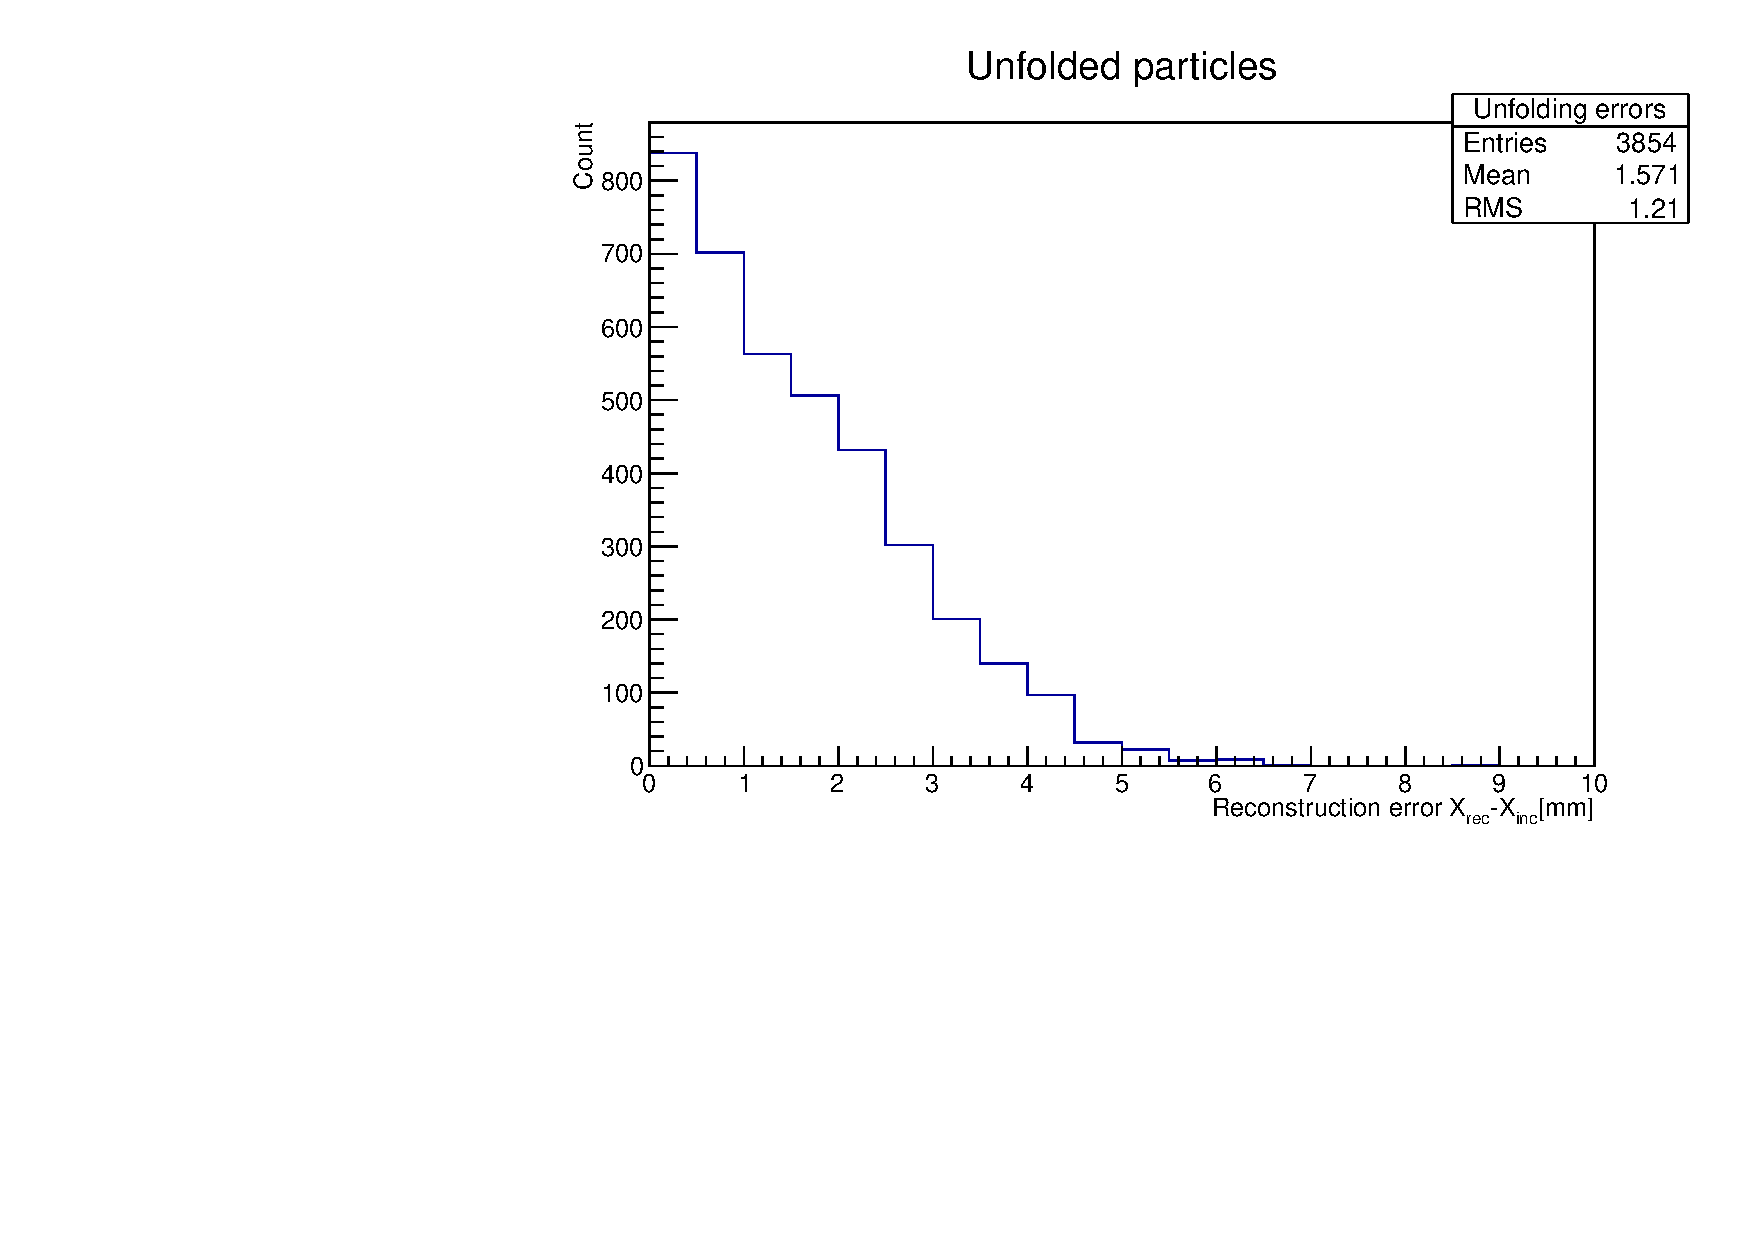
\includegraphics[clip, width=\textwidth]{figure/10_10/x_axis_small_1.pdf}
        \caption{10 + 10 GeV. }
    \end{subfigure}
    ~
    \begin{subfigure}[b]{0.48\textwidth}
        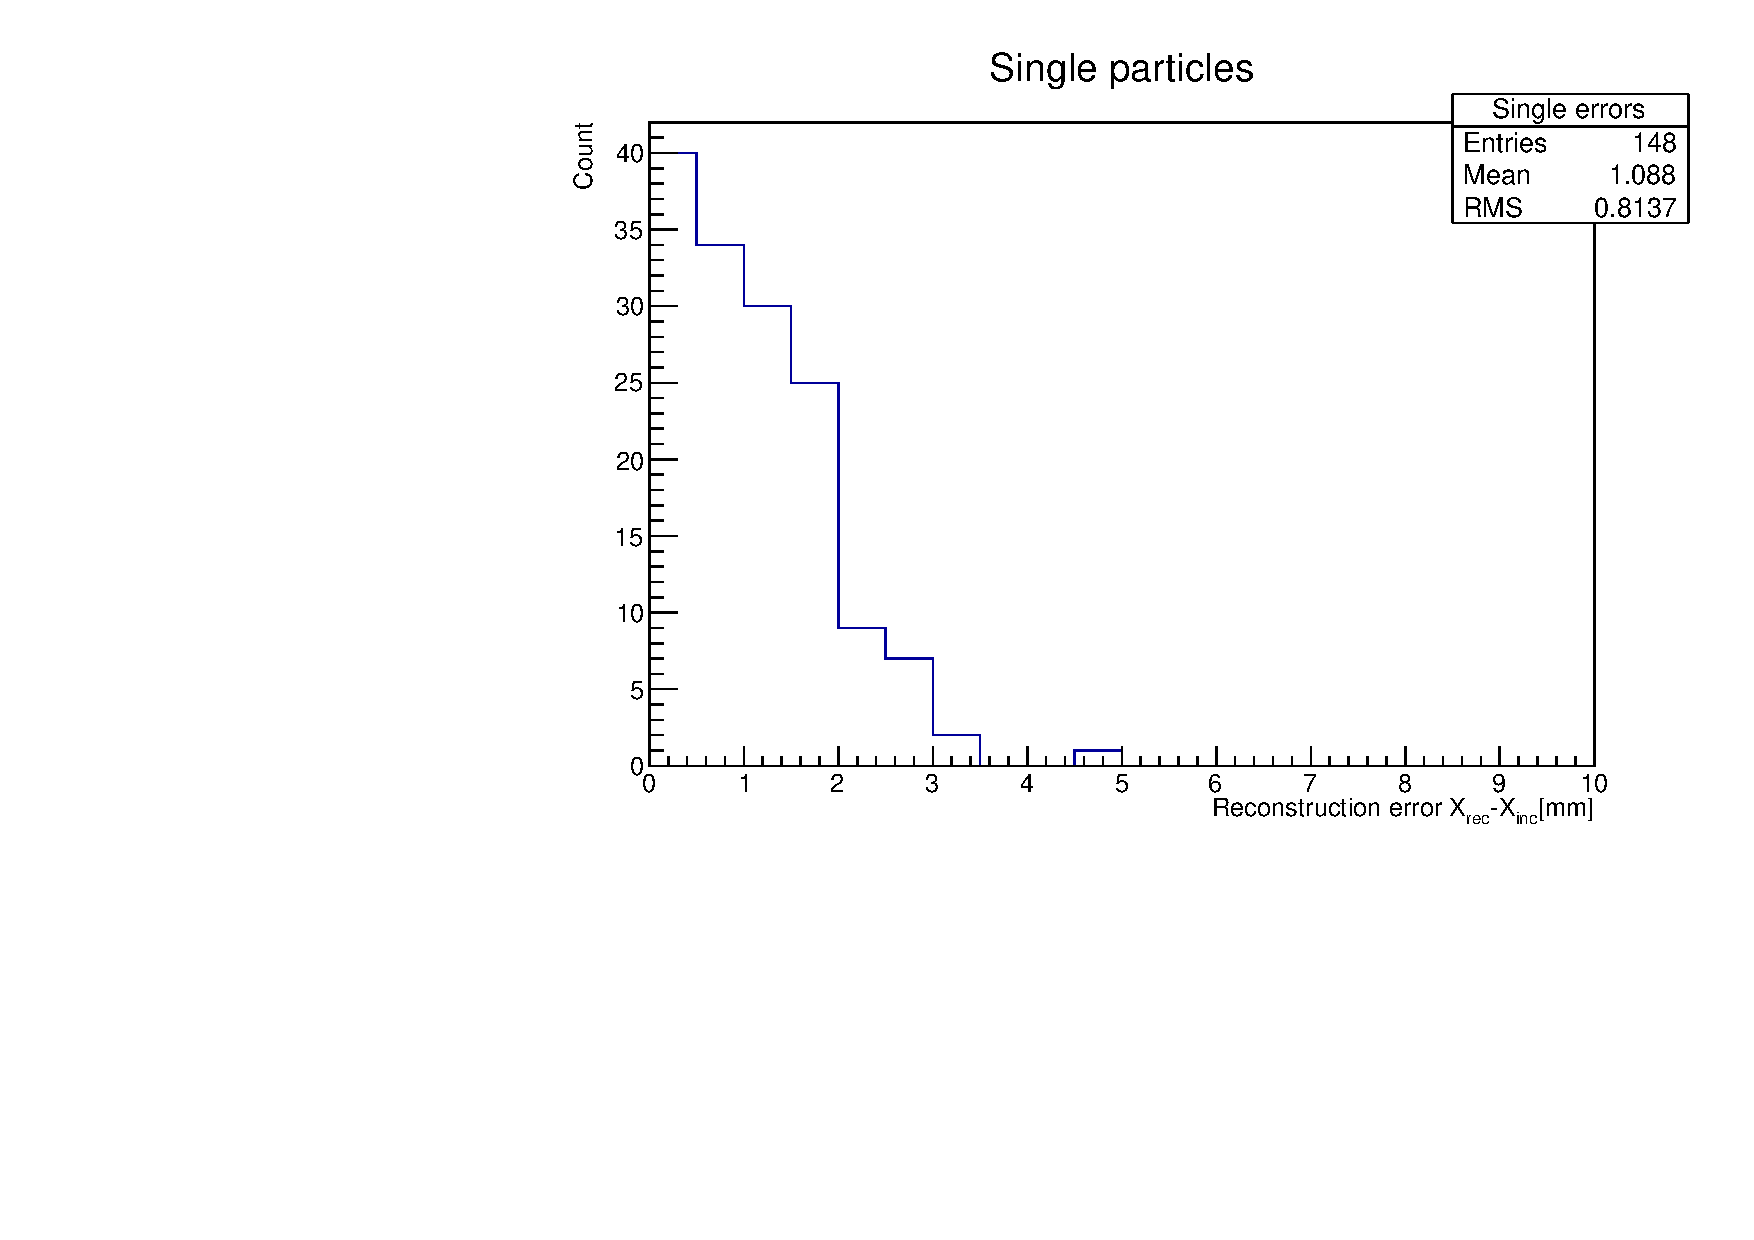
\includegraphics[clip,width=\textwidth]{figure/10_10/x_axis_small_2.pdf}
        \caption{10 + 10 GeV. }
    \end{subfigure}
    ~
    \begin{subfigure}[b]{0.48\textwidth}
        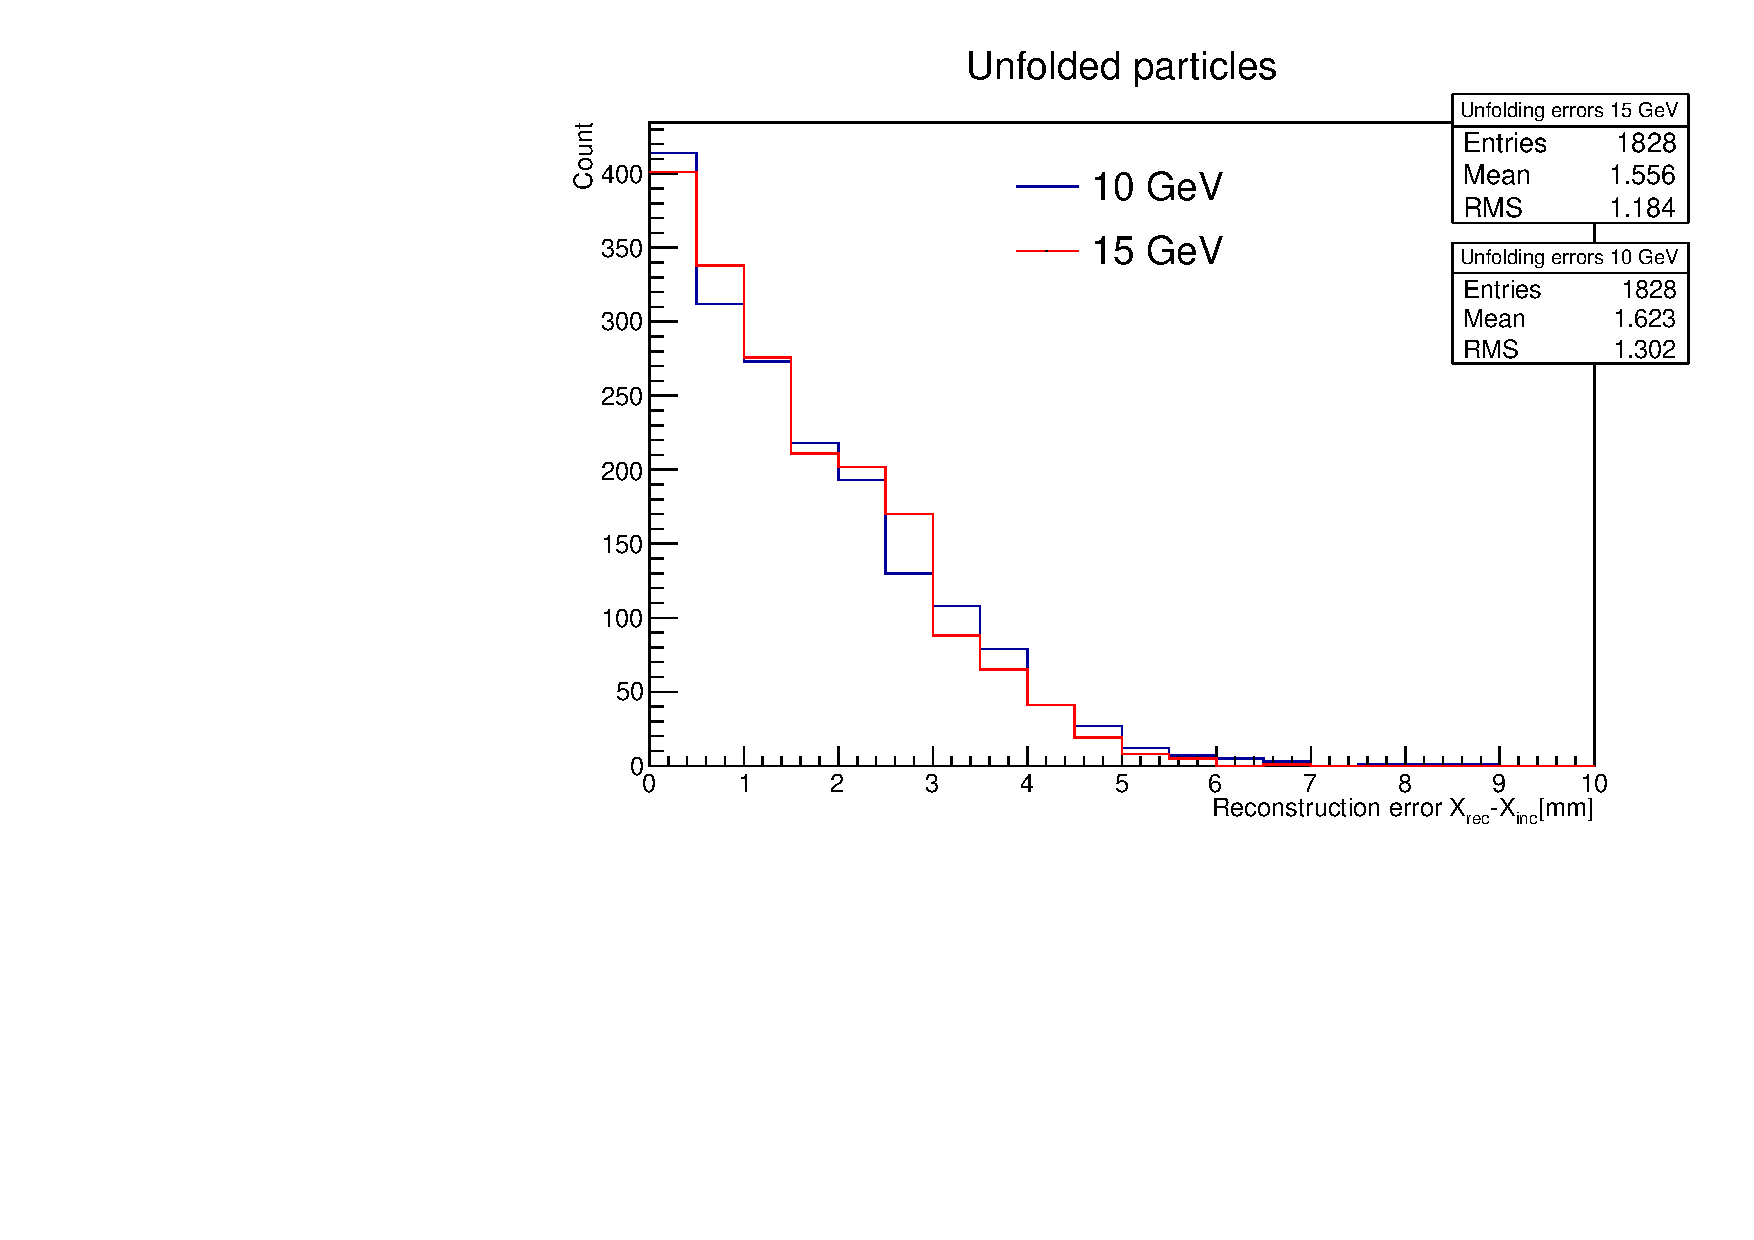
\includegraphics[clip, width=\textwidth]{figure/10_15/x_axis_small_1.pdf}
        \caption{10 + 15 GeV. }
    \end{subfigure}
    ~
    \begin{subfigure}[b]{0.48\textwidth}
        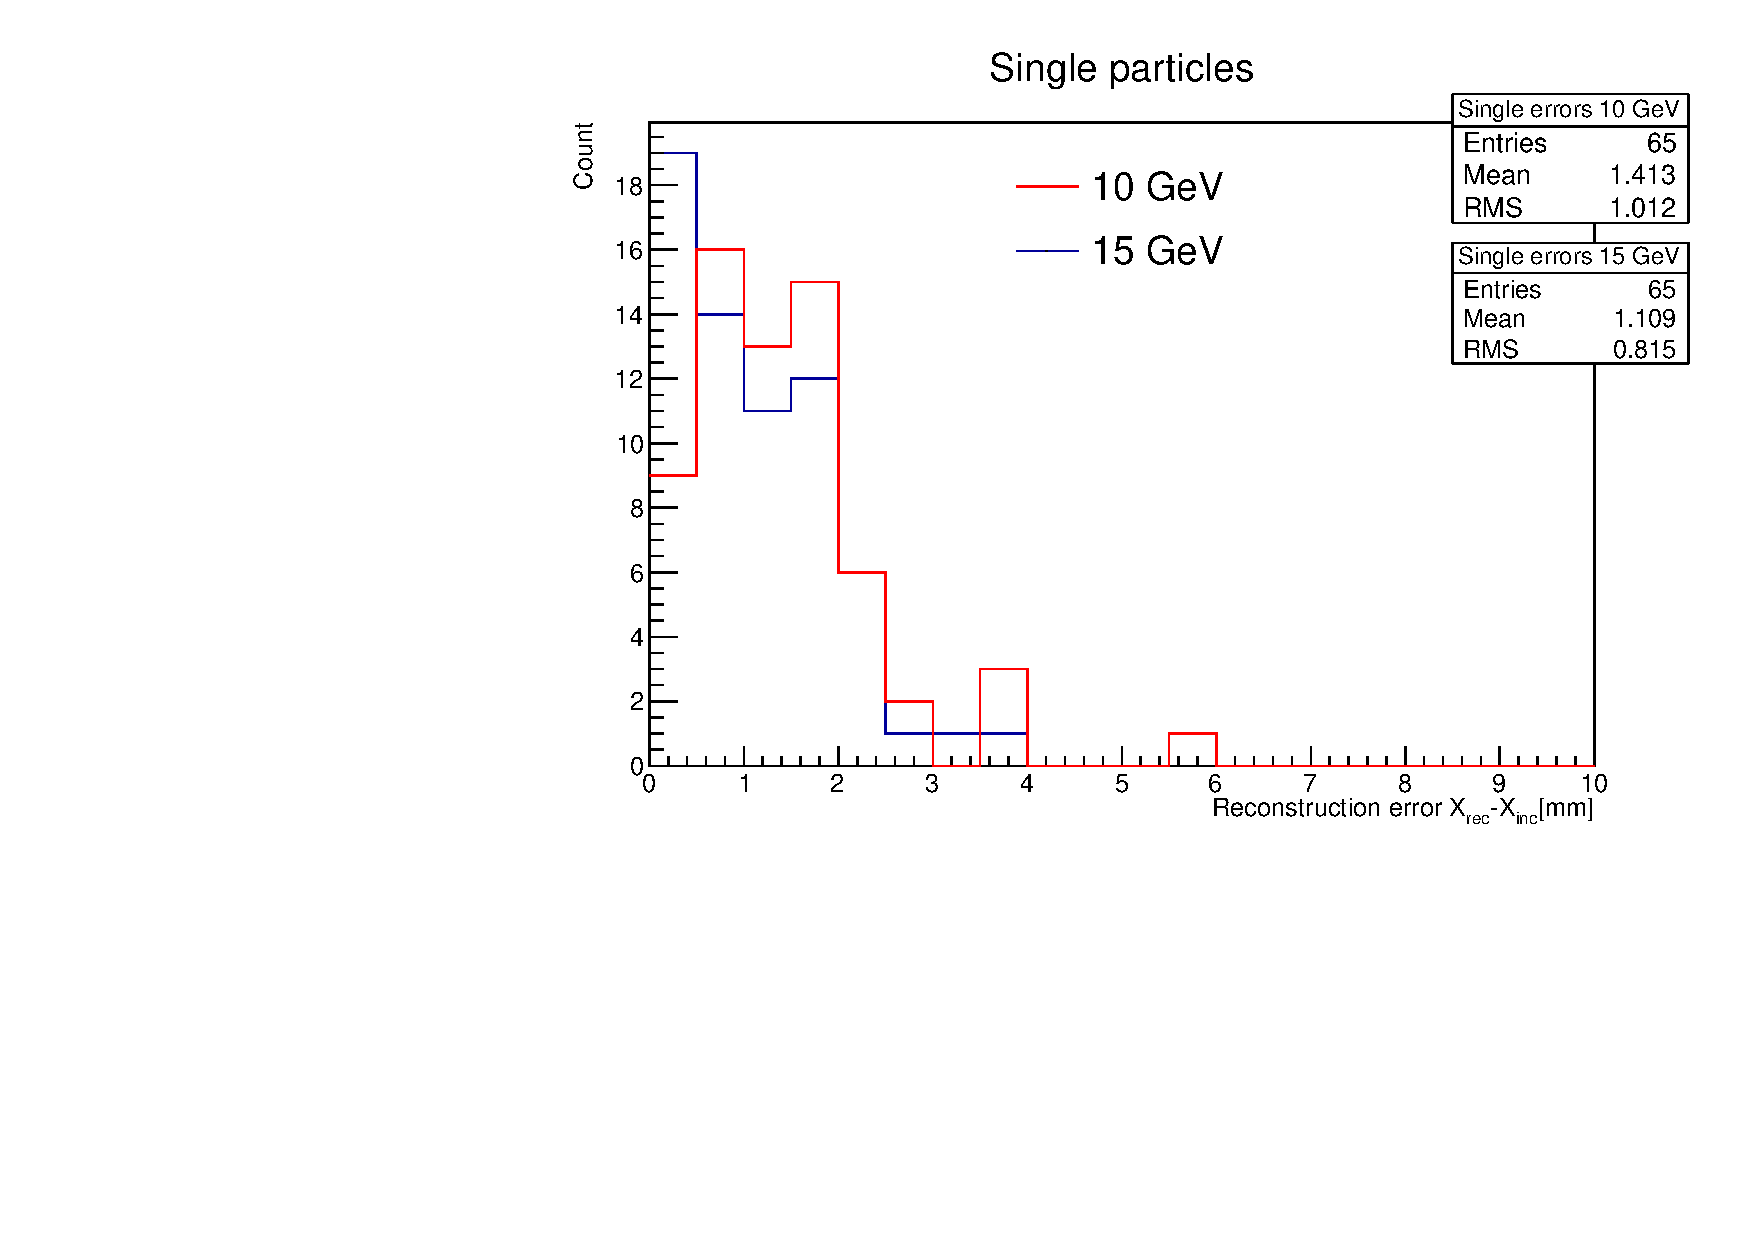
\includegraphics[clip,width=\textwidth]{figure/10_15/x_axis_small_2.pdf}
        \caption{10 + 15 GeV. }
    \end{subfigure}\\
    \caption{Histogramas del error de reconstrucci�n $X_{rec} - X_{inc}$ para varias combinaciones de part�culas $\gamma$. En cada gr�fico se muestra el error para cada una de las part�culas por separado (en el caso de 10+10 GeV s�lo se muestra el error para 10 GeV).}
    \label{fig:reconstruccion}
\end{figure}

Notar que s�lo se present� el error para $X$, los errores en $Y$ son presentados en el Ap�ndice B. El error para el eje $Y$ es mayor que para el eje $X$, la raz�n de esto se estudiar� con mayor profundidad en las conclusiones. 

\subsection{Reconstrucci�n de piones neutros}

Para estudiar la capacidad del detector preshower para detectar piones neutros decayendo en dos gammas muy cercanos entre s� se utilizaron simulaciones de piones lanzados al detector de manera perpendicular. S�lo los piones que decaen y para los cuales ambos gammas llegan al detector fueron considerados. Los piones fueron lanzados desde una distancia de 250~[cm] a la cara frontal del detector. Se utiliz� un rango de energ�a de 10-60 [GeV]. En la Figura~\ref{fig:piones} se observa la fracci�n de part�culas gammas producidas por piones neutros que fueron detectadas como dos part�culas diferentes. Se observa que a mayor energ�a es m�s dif�cil identificar el decaimiento del pi�n neutro como dos part�culas separadas. Esto se debe a que a mayor energ�a, menor el �ngulo de apertura entre los gammas, lo que hace mas dif�cil la identificaci�n. Incluso para energ�as bajas no se identifican la totalidad de piones, esto se produce porque a menor energ�a existe mayor probabilidad de que se produzca un gamma de baja energ�a que no sea identificado por el detector preshower.  

\begin{figure}[t]
\makebox[\textwidth][c]{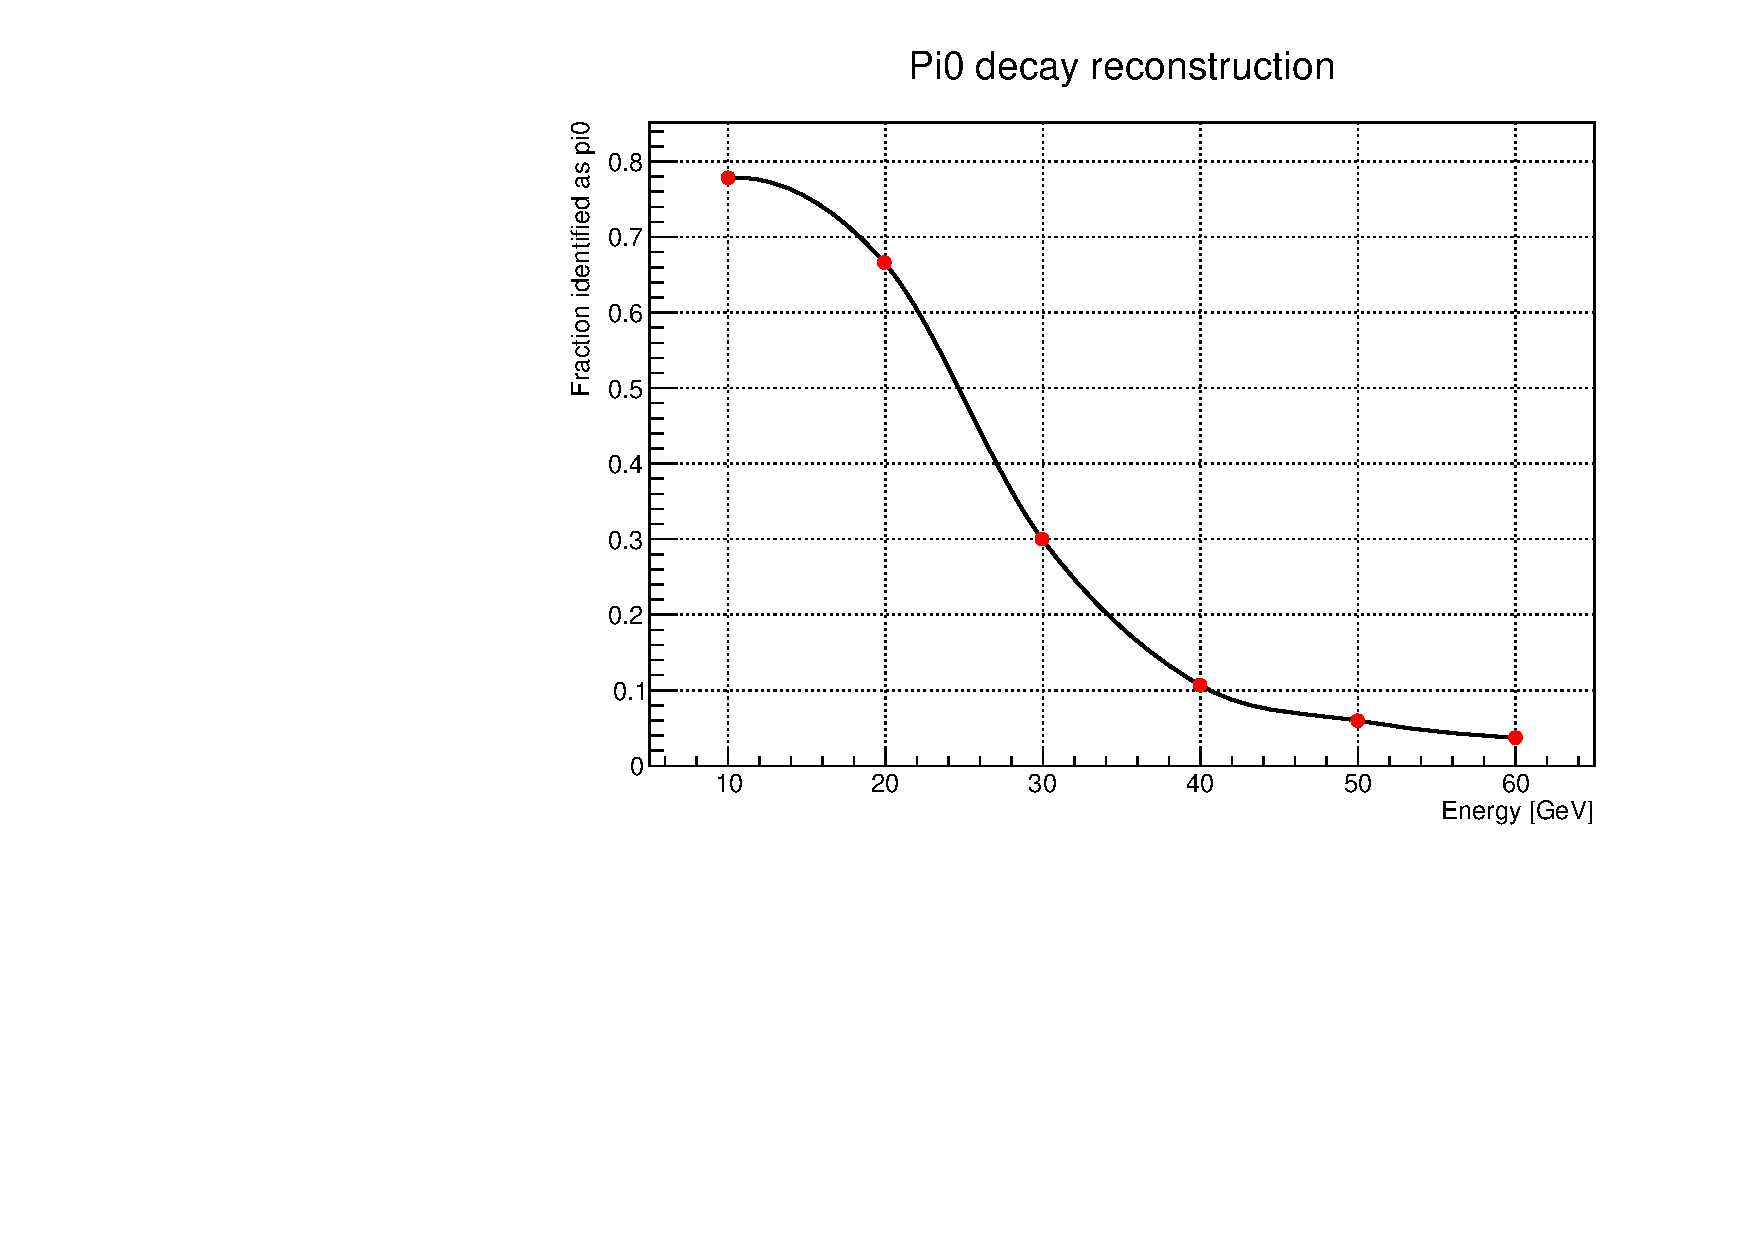
\includegraphics[width=15cm]{figure/pi0_plot.pdf}}
%{\centering 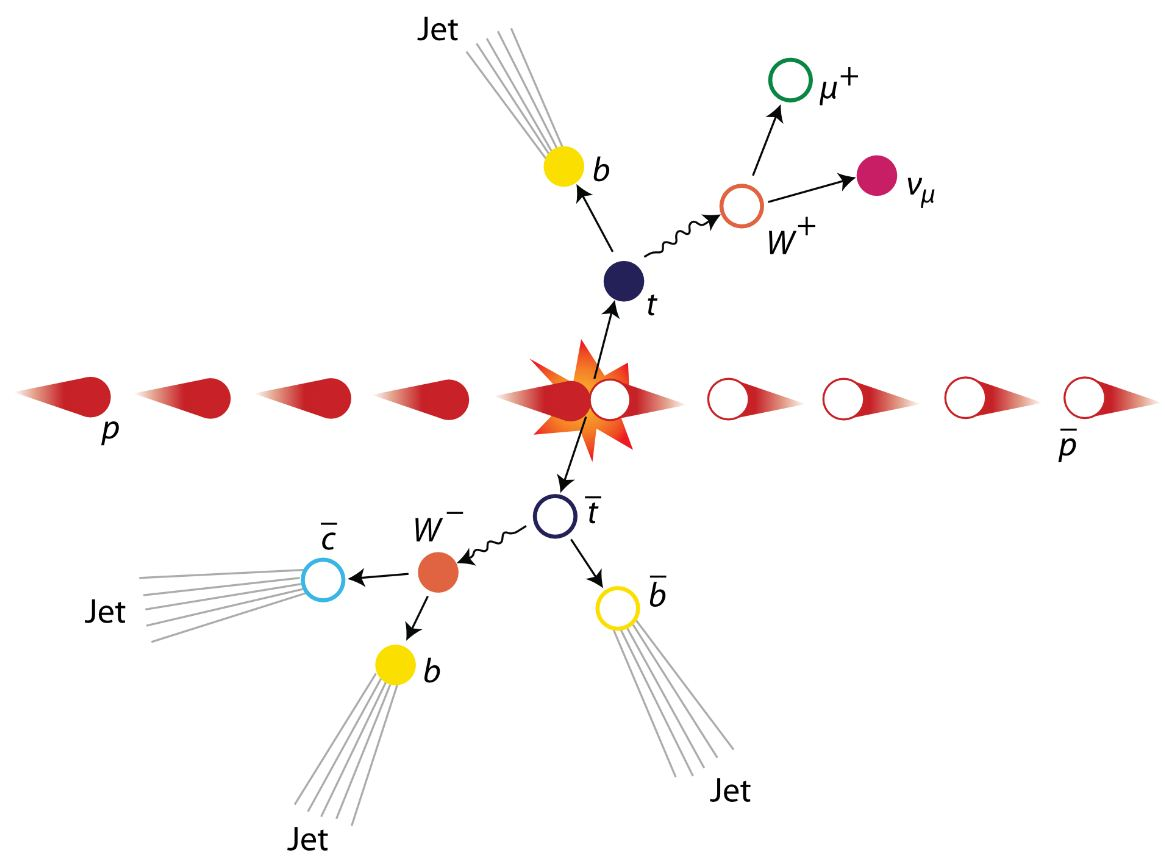
\includegraphics[width=10cm]{figure/collision.JPG}}
\caption[Dos]{ Fracci�n de $\pi^0$ decayendo en dos gammas que golpean el detector y que son identificados como dos gammas por el algoritmo de reconstrucci�n. Se presentan resultados para gammas en el rango de energ�a 10-60 GeV.  \label{fig:piones}}
\end{figure}




    \chapter{Conclusiones y Trabajo Futuro \label{conclusiones}}

En este trabajo hemos propuesto un algoritmo de reconstrucci�n completo para el detector preshower siendo construido por investigadores del Centro Cient�fico y Tecnol�gico de Valpara�so (CCTVal). El algoritmo es capaz de identificar y reconstruir la posici�n de part�culas muy cercanas entre s�. De esta manera soluciona un problema de gran importancia para el trabajo de detecci�n de part�culas en la f�sica de altas energ�as. El algoritmo es, adem�s, capaz de identificar piones neutros decayendo en dos gammas muy cercanos entre s�. Tambi�n, se estudi� el comportamiento del detector preshower en la identificaci�n de part�culas, de esto se pueden concluir algunos puntos de vital inter�s para pr�ximas iteraciones en el dise�o del detector presower.

\begin{itemize}
\item El detector preshower es capaz de identificar part�culas muy cercanas entre s�. La distancia m�nima desde la cual las part�culas pueden ser detectadas como dos part�culas separadas es alrededor de 20 [mm], como se observa en la Figura~\ref{fig:clusters}. Podemos comparar estos resultados a los del detector PHOS, presentados en~\cite{alice1999technical}. Los autores reportan una distancia m�nima para la detecci�n de dos part�culas de 26 [mm], es decir el detector preshower permite una ganancia en resoluci�n de alrededor de 23$\%$.  Esto ya es una ganancia considerable y puede ser mejorada a�n m�s en pr�ximas iteraciones del dise�o del detector. 
\item El algoritmo es capaz de reconstruir la posici�n de las part�culas incidentes. Es posible comparar los resultados en la reconstrucci�n de posici�n a los reportados por PHOS en la referencia mencionada con anterioridad. Ah� se reporta un r.m.s de la distribuci�n de errores ($\sqrt{\sum_i (x_{rec} - x_{inc})^2}$) para part�culas gammas de 1 y 10 GeV con un �ngulo de incidencia de 0 grados de aproximadamente 3.4[mm] y 1[mm]. Para el detector preshower el r.m.s para 1 y 10 GeV para part�culas individuales es de 0.9641[mm] para part�culas de 1[GeV] y 0.9198 para 10 [GeV]. Si bi�n para el caso de 10 [GeV] los errores son parecidos, para 1[GeV] el detector preshower se comporta considerablemente mejor. Esto es debido a que el dise�o de la matriz de cristales del detector Preshower permiten una mejor reconstrucci�n incluso cuando la energ�a de la part�cula incidente es menor.
\item El error de reconstrucci�n es mayor en el eje Y que en el eje X. Esto se entiende principalmente por dos razones. Seg�n el modelo de la ecuaci�n~\ref{eq:modelo} que considera los efectos de la electr�nica y dise�o f�sico del detector, la varianza de la propagaci�n de la energ�a en el eje Y es mayor que en el eje X.  Esto se debe a factores electr�nicos y f�sicos fuera del alcance del algoritmo de reconstrucci�n (por ejemplo, diferencias en el aislamiento de las fibras que transportan los fotones). El efecto de ensanchamiento de las lluvias se puede observar claramente en la Figura~\ref{fig:peaks}. Esto dificulta la reconstrucci�n de posici�n produciendo errores mayores en el eje Y. 

Otra raz�n de esta diferencia es el m�todo de resoluci�n de ambig�edades. Seg�n el funcionamiento actual del algoritmo, cuando dos part�culas son observadas en ambos ejes se resuelve el problema de ambig�edad mediante el uso de la diferencia de conteo de fotones entre las lluvias detectadas en cada eje. Como se mencion� al presentar el m�todo este algoritmo no funciona en el caso que ambas part�culas depositen una cantidad de energ�a similar. Aunque estos casos son poco probables, al ocurrir producen una mala elecci�n de posiciones en el eje Y (el algoritmo funciona emparejando posiciones en el eje Y a las posiciones reconstruidas en el eje X) lo que a su vez produce errores de reconstrucci�n muy mayores a la media (para un mayor an�lisis de este problema el lector se puede dirigir al Ap�ndice B, Figura~\ref{fig:errores_y}).

\item El detector preshower por s� s�lo no puede manejar la situaci�n en las que el �ngulo de incidencia es no perpendicular a la cara frontal del detector. Para lograr esto otros tipos de detectores implementan m�todos como la segmentaci�n transversal o la medici�n de los tiempos en los que la part�cula atraviesa el detector. Diferentes �ngulos de incidencia afectan los resultados del preshower. Por ejemplo, el error medio para part�culas individuales de 10 GeV es de 0.7402 [mm] cuando el �ngulo de incidencia es de 0 grados. En cambio, si el �ngulo es 6 grados el error medio pasa a ser 3.573 [mm]. Si bien el detector preshower no es capaz de solucionar este problema por s� solo, otras secciones podr�an medir el �ngulo de incidencia y mediante estas mediciones implementar correcciones de posici�n para los valores medidos por el detector preshower. 

\end{itemize}

En base a esto se propone como trabajo futuro:

\begin{itemize}
\item Se ha observado que un importante factor que afecta la capacidad del algoritmo para reconstruir la posici�n de la part�cula incidente de una manera precisa (especialmente en el eje Y) y que adem�s afecta la capacidad de identificar part�culas incidentes cercanas es el ensanchamiento de las lluvias debido a factores electr�nicos de la detecci�n. Este efecto se refleja en el modelo de propagaci�n utilizado para simular las mediciones del MPPC de la ecuaci�n~\ref{eq:modelo}. Esto conforma una mayor conclusi�n de este trabajo: Pr�ximas iteraciones del dise�o del detector preshower debiesen intentar mejorar estos valores, lo que producir� una mejora directa en la capacidad para identificar part�culas cercanas y la precisi�n de la reconstrucci�n del detector preshower.

\item El algoritmo de resoluci�n de ambig�edades es un foco claro para implementar mejoras al algoritmo de reconstrucci�n. Primero, es necesario implementar un algoritmo que funcione para un n�mero cualquiera de part�culas incidentes. El foco principal de este trabajo es producir un algoritmo funcional para las primeras etapas de prueba del detector preshower, en donde se desea medir su eficacia en la reconstrucci�n de dos part�culas gammas cercanas entre s�. Para etapas posteriores es necesario solucionar el problema de ambig�edad de una manera m�s general, lo que sin embargo, queda fuera del foco de este trabajo. Adem�s, posibles mejoras pueden ser introducidas mediante m�todos m�s avanzados de emparejamiento de lluvias electromagn�ticas, por ejemplo utilizando no s�lo el valor de fotoelectrones medidos, sino que tambi�n variables derivadas de la forma de las lluvias. Todo esto se deja como trabajo futuro.

\item Problemas como la p�rdida de precisi�n para �ngulos diferentes a cero peden ser solucionados mediante el trabajo conjunto del detector preshower con el resto de la cadena de detecci�n. Esto s�lo puede ser considerado en un contexto m�s amplio, teniendo un conocimiento m�s preciso del uso final del detector preshower. En la etapa actual de producci�n no se conoce la constituci�n final de la cadena de detecci�n, por lo que este tipo de trabajo solo se puede hacer en base a supuestos. Es por esto que esto deja como trabajo futuro.

\item Aunque en este trabajo s�lo se consider� que dos part�culas son identificables cuando forman dos clusters separados o dos m�ximos separables mediante el algoritmo de unfolding, es posible identificar dos part�culas incluso cuando s�lo un cluster es observado. Esto se realiza mediante la consideraci�n de la forma de las lluvias formadas. Es de esperar que una lluvia formada por dos part�culas sea m�s ancha que la formada por una sola. Aunque esto se puede realizar mediante cortes relativamente simples a valores como la varianza de la lluvia, los m�todos actuales para la identificaci�n de part�culas se basan en el uso de algoritmos de aprendizaje (por ejemplo~\cite{aurisano2016convolutional}) que mediante la utilizaci�n de varias variables que resumen la forma de la lluvia son capaces de identificar el tipo o n�mero de part�culas. Por otro lado, este tipo de identificaci�n puede ser realizada en otras capas de detecci�n, por ejemplo en un calor�metro completo, capaz de tener una imagen m�s precisa de la forma de la lluvia electromagn�tica. Experimentos iniciales han sido realizados en este camino utilizando una red neuronal que es capaz de aprender a identificar si la lluvia procede de una o m�s part�culas analizando variables como la varianza de la lluvia, el valor de la raz�n entre el peak y la energ�a total, el sesgo de la lluvia, entre otras. Mas experimentaci�n se necesita en este punto y se deja como trabajo futuro.
\end{itemize}


    %\include{5_experimentos/4_Experimentos}
    %\include{6_conclusion/5_Conclusion}

    \clearpage % o \cleardoublepage
    \addappheadtotoc
    \appendixpage
    \appendix
    \chapter{Conceptos B�sicos}

En esta secci�n se presentar� una breve descripci�n de los conceptos f�sicos relevantes para comprender de una manera general el dise�o y funcionamiento del detector Preshower. La finalidad de esta secci�n es entregar al lector, con conocimientos b�sicos en f�sica moderna, los conceptos principales que le permitir�n comprender de manera general las decisiones de dise�o tanto en la construcci�n del detector, pero principalmente, en la propuesta de algoritmo de reconstrucci�n. Para mayor informaci�n y un tratamiento m�s t�cnico de los temas el lector se puede dirigir a \cite{soria2011fisica,leo2012techniques,green2000physics}.

\section{Paso de part�culas por la materia}
El estudio de las interacciones de las part�culas con la materia constituye la base del estudio de los detectores. Un detector detectar� una part�cula mediante las interacciones que esta tiene con los materiales del detector, por lo que el estudio de las principales interacciones de las part�culas con la materia es indispensable para entender el funcionamiento de los detectores.

\subsection{Secci�n eficaz y recorrido libre}
La secci�n eficaz es un concepto fundamental en la f�sica de part�culas. Este se relaciona con la probabilidad de interacci�n de un part�cula con un blanco. Considerar un haz de part�culas que incide en un blanco de modo que son dispersadas (en parte) en un �ngulo $\theta$ en direcci�n de un detector, siendo el blanco de �rea $A$ menor que la superficie del haz. Considerar que el flujo de part�culas en el haz es $F[cm^{-2}s^{-1}]$ (n�mero de part�culas por unidad de �rea y por unidad de tiempo). Adem�s considerar que el blanco $X$ es muy delgado ($\delta x$), de manera que la probabilidad de que las part�culas del blanco se posicionen una delante de otra es baja. Tambi�n, el blanco tiene una densidad de $N$ part�culas, es decir que el haz incidente ver� $N\delta x$ part�culas. Sea, $N_s$ el n�mero promedio de part�culas dispersadas en el �ngulo $d\Omega$ del detector, entonces se puede definir la secci�n eficaz diferencial como:
\begin{equation}
\frac{d\sigma}{d\Omega} (E, \Omega) = \frac{1}{F}\frac{dN_s}{d\Omega}, \nonumber
\end{equation}
que es la fracci�n promedio de part�culas dispersadas hacia $d\Omega$ por unidad de tiempo y por unidad de flujo. La secci�n eficaz total se define como 
\begin{equation}
\sigma(E) = \int d\Omega \frac{d\sigma}{d\Omega}.\nonumber
\end{equation}
Ahora, debido a que el �rea del blanco es menor que el haz, el n�mero de part�culas que pueden interactuar del haz es $N_{inc}=FA$ y el n�mero promedio de part�culas dispersadas en $d\Omega$ es:
\begin{equation}
N_s(\Omega) = FAN\delta x \frac{d\sigma}{d\Omega},\nonumber
\end{equation}
entonces, el n�mero de part�culas dispersadas en todos los �ngulos es
\begin{align}
N_{tot} &= FAN\delta x \sigma  \\ \nonumber
 &= N_{inc}N\delta x \sigma,\nonumber
\end{align}
de esta manera se puede definir la probabilidad de interacci�n de una part�cula en un material de espesor $\delta x$ como
\begin{equation} \label{eq:prob}
\frac{N_{tot}}{N_{inc}} = n\sigma\delta x,
\end{equation}
es decir que la secci�n eficaz es proporcional a la probabilidad de interacci�n del haz incidente con el blanco.
El concepto de secci�n eficaz es fundamental y constituir� el valor principal para evaluar las posibles interacciones presentes en el detector. 
Se puede, tambi�n, calcular la \emph{distancia media recorrida} por una part�cula en un material de cualquier grosor $x$. Considerar $P(x)$ como la probabilidad de que una part�cula no tenga interacci�n en una distancia $x$ de material y $w dx$ como la probabilidad de tener una interacci�n entre $x$ y $dx$. La probabilidad de no tener una interacci�n entre $x$ y $x+dx$ es
\begin{align}
P(x + dx)=&  P(x)(1-wdx),\nonumber \\ 
P(x) + \frac{dP(x)}{dx}dx =&  P(x) - P(x)wdx,\nonumber\\ 
dP(x) =&  -wP(x)dx. \nonumber
\end{align} 
Resolviendo la ecuaci�n diferencial anterior y requiriendo que $P(0) = 1$ se obtiene que 
\begin{equation}
P(x) = exp(-wx). \nonumber
\end{equation} 
Finalmente, es posible calcular la distancia media recorrida por una part�cula en un material como
\begin{align}
\lambda &= \frac{\int xP(x)dx}{\int P(x) dx}\nonumber \\ 
 &= \frac{1}{w}\nonumber \\ 
 &= \frac{1}{N\sigma}. \nonumber
\end{align} 
Usando la ecuaci�n \ref{eq:prob} y el hecho de que la probabilidad de interacci�n en un blanco delgado puede ser expandida como
\begin{align}
P_{int}(\delta x) &= 1 - exp(-wx),\nonumber\\ 
&= 1-\bigg(1-\frac{\delta x}{\lambda} + ...\bigg),\nonumber\\ 
&\simeq \frac{\delta x}{\lambda}. \nonumber
\end{align} 
Entonces, la probabilidad de supervivencia queda como
\begin{equation}
P(x) = e^{-x/\lambda}. \nonumber
\end{equation}
El valor $\lambda$ tambi�n se conoce como longitud de atenuaci�n y se puede entender como la distancia a la cual la probabilidad de que la part�cula no sea absorbida cae en $1/e$.
La longitud de atenuaci�n es un valor importante para evaluar y comprar diferentes materiales utilizados como productores de lluvia en un detector calor�metro.

En la siguiente secci�n se analizar�n las interacciones de part�culas con la materia �tiles para comprender el funcionamiento del detector preshower.
\subsection{Interacci�n de part�culas con la materia}
Las part�culas pueden interactuar de muchas maneras con la materia, muchas de estas interacciones est�n muy estudiadas y sus secciones eficaces son conocidas. En este trabajo nos concentraremos en las interacciones sufridas por fotones y electrones que pudiesen tener influencia en el funcionamiento y posterior reconstrucci�n del detector preshower. El detector preshower es un detector del tipo calor�metro que produce lluvias electromagn�ticas (esto se proceder� a explicar en mayor detalle m�s adelante), por lo que son las interacciones involucradas en esto las que interesaran en este trabajo.
\subsubsection{Interacci�n de part�culas con �tomos}
En este caso la part�cula incidente interact�a directamente mediante colisiones con el �tomo. Se pueden dar dos casos, una colisi�n con los electrones del �tomo, de manera que el �tomo queda ionizado y la part�cula incidente pierde energ�a, o una colisi�n el�stica con el n�cleo del �tomo, donde la part�cula incidente cambia de direcci�n y pierde un poco de energ�a (despreciable). La perdida de energ�a por colisi�n con electrones es modelada por la f�rmula \emph{Bethe-Bloch} mientras que las colisiones con los n�cleos, en la que es mas probable que la part�cula incidente cambie de direcci�n, es modelada por la f�rmula de \emph{Rutherford}.
\subsubsection{Interacci�n de electrones y positrones}
Para electrones y positrones otra interacci�n del tipo electromagn�tica, conocida como radiaci�n de frenado (o \emph{bremsstahlung}), afecta a la part�cula incidente (adem�s de las interacciones por colisi�n), por lo que la perdida energ�a total ser�
\begin{equation}
\frac{dE}{dx} = \bigg(\frac{dE}{dx}\bigg)_{col} + \bigg(\frac{dE}{dx}\bigg)_{rad}. \nonumber 
\end{equation} 
La radiaci�n de frenado (o \emph{bremsstrahlung}) sucede en presencia de un campo el�ctrico intenso. En este los electrones son frenados y emiten fotones, perdiendo energ�a. Es la principal causa de p�rdida de energ�a a altas energ�a. El electron incidente con energ�a $E_i$ emite un fot�n de energ�a $E_\gamma = E_i - E_f$ donde $E_f$ es la energ�a final del electr�n. Es posible demostrar que la p�rdida de energ�a por la radiaci�n de frenado es linealmente proporcional con $E_i$. Adem�s, a altas energ�as la secci�n eficaz de la radiaci�n de frenado es casi constante y es posible definir la \emph{longitud de radiaci�n} $X_0$ como 
\begin{equation}
\frac{1}{X_0} = n_\alpha \sigma_{rad}, \nonumber
\end{equation} 
donde $n_\alpha$ es el n�mero de �tomos por $cm^3$ en el material y $\sigma_{rad}$ la secci�n eficaz de la radiaci�n de frenado. Es posible demostrar que 
\begin{equation}
E = E_0 e^{-x/X_0}, \nonumber
\end{equation} 
es decir, el valor $X_0$ representa la distancia media recorrida en la que el electr�n ha disminuido a $1/e$ de su valor de energ�a inicial mediante el proceso de bremsstahlung. La longitud de radiaci�n depende del material y ser� un valor importante a considerar al dise�ar un detector.

El positr�n, al igual que el electr�n, pierde energ�a por ionizaci�n y radiaci�n de frenado, sin embargo, a muy baja velocidad puede formar un \emph{positronio} con el electr�n, un part�cula muy parecida a un �tomo de hidr�geno pero con estados menos espaciados. El positronio se aniquila con secci�n eficaz $\sigma_{an}$ produciendo dos fotones de $0.511 MeV$, 
\begin{equation}
e^+ + e^- \rightarrow \gamma + \gamma, \nonumber
\end{equation} 
aunque tambi�n se pueden producir tres gammas finales (dependiendo del estado del positronio).

\subsubsection{Interacci�n de part�culas gamma}
Los fotones pueden interactuar de varias maneras con la materia, estas interacciones pueden producir part�culas cargadas que permitir�n identificar al fot�n. Las interacciones de fotones con la materia pueden ser por efecto fotoel�ctrico, efecto Compton, creaci�n de pares, difusi�n Rayleigh con un electr�n del material y absorci�n fotonuclear. Los dos �ltimos procesos son poco frecuentes en el rango de energ�a importante para este trabajo por lo que no se analizar�n. 

El efecto fotoel�ctrico ocurre cuando un fot�n es absorbido por un electr�n del �tomo, obteniendo este �ltimo la energ�a del fot�n incidente, si esta energ�a supera la funci�n de trabajo del material, el electr�n es liberado del �tomo. Los electrones liberados de esta manera son llamados fotoelectrones, para diferenciarlos de los electrones incidentes. La energ�a del electr�n liberado es $E_e = E_\gamma - E_b$, donde $E_b$ es la funci�n de trabajo y $E_\gamma$ es la energ�a del fot�n que es igual a $E_\gamma = h\nu$.

Por otro lado, el efecto de Compton se trata de una difusi�n el�stica del fot�n con un electr�n que act�a como si estuviese libre, $\gamma + e_- \rightarrow \gamma' + e'_-$. El fot�n sale en un �ngulo $\theta$ y con una nueva longitud de onda $\lambda'$, dada por $\lambda' - \lambda = \frac{h}{mc}(1-\cos\theta)$. Un diagrama de la interacci�n se muestra en la Figura \ref{fig:compton}.

\begin{figure}[t]
\makebox[\textwidth][c]{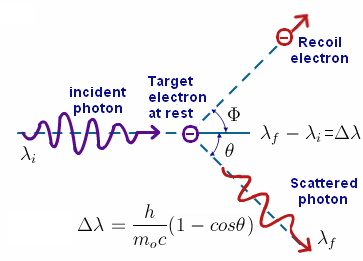
\includegraphics[width=8cm]{figure/compton2.png}}
%{\centering 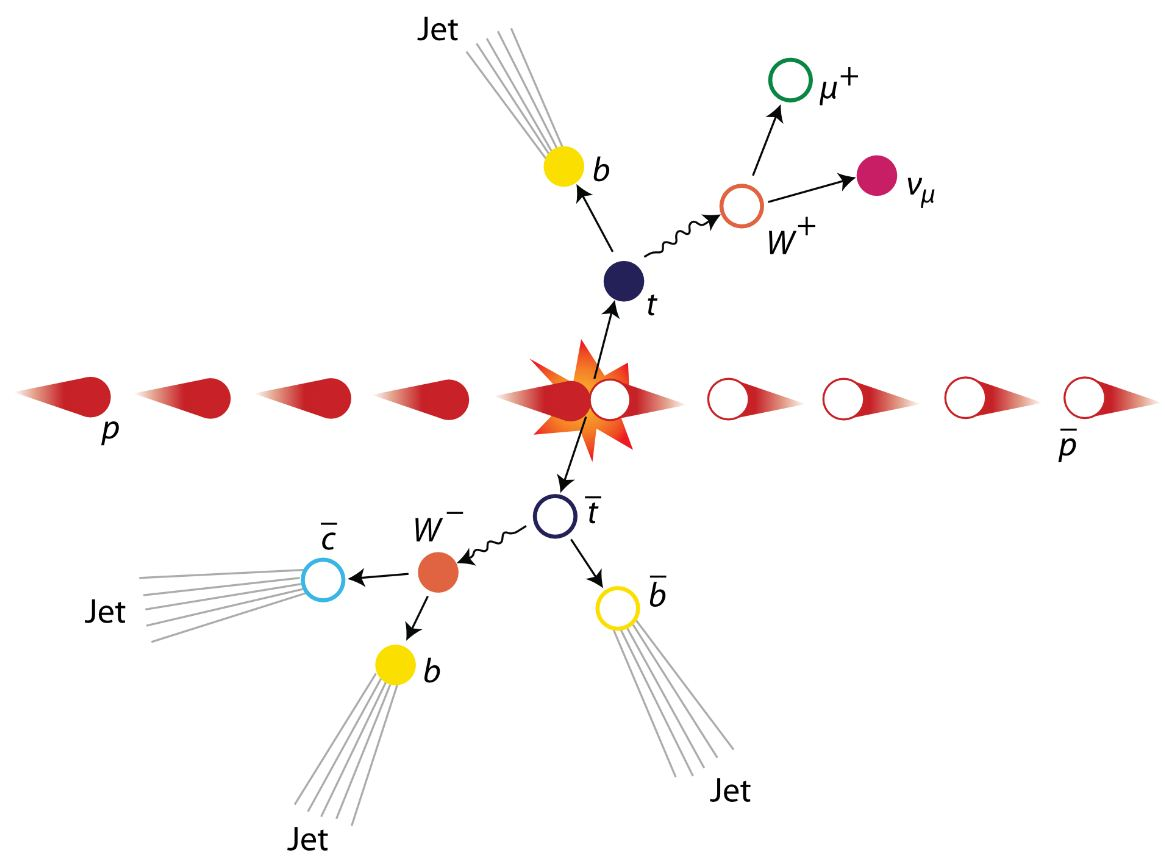
\includegraphics[width=10cm]{figure/collision.JPG}}
\caption[Colisi�n entre part�culas y part�culas secundarias producidas]{Diagrama del efecto compton entre un fot�n y un electr�n.\label{fig:compton}}
\end{figure}


La creaci�n de pares, proceso mediante el cual un fot�n produce un electr�n y un positr�n, $\gamma \rightarrow e^+ + e^-$, sucede en presencia de un campo el�ctrico intenso. Para que esto ocurra es necesario que la energ�a del fot�n cumpla que $E_\gamma \geq 1.022 MeV$. El �ngulo de emisi�n del par $e^\pm$ respecto al fot�n a alta energ�a sigue $\theta \sim \frac{mc^2}{E_\pm}$, por lo que a mayor energ�a menor el �ngulo de emisi�n.

A altas energ�as la creaci�n de pares es el proceso dominante, con secci�n eficaz $\sigma_{par}$ constante. Al igual que para el electr�n se puede introducir la longitud de conversi�n (atenuaci�n) $X_c$ como
\begin{equation}
\frac{1}{X_c} = n_\alpha \sigma_{par} = \frac{1}{\frac{9}{7}X_0}. \nonumber
\end{equation}
Adem�s, se cumple que la intensidad del haz de fotones se comporta en funci�n de $X_c$ como
\begin{equation}
I = I_0 e^{-x/X_c}. \nonumber
\end{equation}
 En la Figura \ref{fig:cross_section} se muestran diferentes longitudes de atenuaci�n dada la energ�a del fot�n incidente, para cada uno de los procesos analizados. La figura muestra longitudes de atenuaci�n comunes que deben ser adaptadas dependiendo del material. En esta se observa claramente como la producci�n de pares predomina a altas energ�as, mientras que en la regi�n de bajas energ�as el proceso predominante es el efecto fotoel�ctrico.

\begin{figure}[t]
\makebox[\textwidth][c]{\includegraphics[width=14cm]{figure/crosssection_2.png}}
%{\centering \includegraphics[width=10cm]{figure/collision.JPG}}
\caption[Colisi�n entre part�culas y part�culas secundarias producidas]{Longitud de atenuaci�n para diversos procesos de un fot�n.\label{fig:cross_section}}
\end{figure}


    \chapter{Resultados adicionales}
\label{ApendiceB}
En esta secci�n se presentar�n resultados adicionales del funcionamiento del algoritmo de reconstrucci�n.

\section{Reconstrucci�n de posici�n}

Como una forma de comprender mejor el funcionamiento del algoritmo de reconstrucci�n, podemos analizar los errores de reconstrucci�n para cada una de las posibilidades que se dan al reconstruir dos part�culas: 
\begin{enumerate}
\item S�lo una part�cula es identificada de manera err�nea.
\item Un cluster es identificado en uno de los ejes y en el otro un cluster con dos m�ximos.
\item Dos clusters son identificados en un eje y en el otro un cluster con un m�ximo.
\item Dos clusters separados son identificados en ambos ejes.
\item Dos clusters en un eje y en el otro un cluster con dos m�ximos.
\item Un cluster con dos m�ximos en ambos ejes.
\end{enumerate}

El algoritmo de unfolding debe ser aplicado en los casos 2, 5 y 6. Mientras que la resoluci�n de ambig�edades utilizando el conteo de fotoelectrones debe ser aplicada en los casos 3 y 6.

En la Figura~\ref{fig:10_1_errores} y~\ref{fig:10_10_errores} se presentan histogramas para el error de reconstrucci�n para cada uno de estos casos y para las combinaciones de part�culas de 10+1 GeV y 10+10 GeV. En el Cuadro~\ref{tab:errores_extra} se presentan los valores resumidos para el error de reconstrucci�n para las combinaciones de part�culas 10+1, 10+5, 10+10 y 10+15 GeV y para cada uno de los casos enumerados anteriormente. 

\begin{table}[h]
\centering
\begin{tabular}{|p{1cm} p{1cm}| p{1.8cm} |p{1.8cm} |p{1.8cm} |p{1.8cm}| p{1.8cm}| p{1.8cm} |}
\hline
    &  & \multicolumn{6}{c|}{Resoluci�n posici�n [mm]} \\\hline
\multicolumn{2}{|c|}{Energias  [GeV]} & Caso 1 & Caso 2 & Caso 3 & Caso 4 & Caso 5 & Caso 6  \\ \hline
\multirow{2}{*}{10 + 1} & 10  & 3.807 $\pm$ 5.137 & 2.1 $\pm$ 2.523 & 1.876 $\pm$ 2.66 & 1.382 $\pm$ 0.7241 & 1.632 $\pm$ 1.135 & 2.253 $\pm$ 1.081 \\ 
 & 1  & 8.862 $\pm$ 7.829  & 3.603 $\pm$ 4.685 & 3.032 $\pm$ 4.503  & 1.035 $\pm$ 0.4122  & 1.68 $\pm$ 1.357 & 3.093 $\pm$ 1.394 \\ \hline
\multirow{2}{*}{10 + 5} & 10  & 5.224 $\pm$ 6.268 & 2.538 $\pm$ 3.169 & 2.105 $\pm$ 2.943 & 1.18  $\pm$ 0.6835 & 2.051 $\pm$ 1.692 & 2.407 $\pm$ 1.103 \\ 
 & 5  & 6.936 $\pm$ 7.14  & 2.996 $\pm$ 3.798 & 3.187 $\pm$ 4.803  & 0.6828 $\pm$ 0.33  & 1.7 $\pm$ 1.043 & 2.67 $\pm$ 1.129 \\ \hline
 \multirow{2}{*}{10 + 10} & 10  & 6.397 $\pm$ 6.915 & 2.617 $\pm$ 3.588 & 2.773 $\pm$ 4.963 & 1.132  $\pm$ 0.7415 & 2.039 $\pm$ 1.408 & 2.526 $\pm$ 1.101 \\ \hline
 \multirow{2}{*}{10 + 15} & 10  & 5.929 $\pm$ 6.585 & 2.819 $\pm$ 3.709 & 3.153 $\pm$ 4.502 & 0.7519  $\pm$ 0.0 & 1.795 $\pm$ 0.9704 & 2.665 $\pm$ 1.424 \\ 
 & 15  & 5.656 $\pm$ 6.585  & 2.628 $\pm$ 3.471 & 2.145 $\pm$ 3.18  & 0.6303 $\pm$ 0.0  & 1.665 $\pm$ 0.9577 & 2.449 $\pm$ 1.088 \\ \hline
 \end{tabular}
\caption{Error de reconstrucci�n para part�culas $\gamma$ para cada uno de los casos del algoritmo. Se presentan resultados para part�culas de 1, 5, 10 y 15 GeV.  \label{tab:errores_extra}}
\end{table}


\begin{figure}
    \centering
    \begin{subfigure}[b]{0.48\textwidth}
        \includegraphics[clip, width=\textwidth]{figure/10_1/x_axis_1.pdf}
        \caption{Una part�cula identificada. }
    \end{subfigure}
    ~
    \begin{subfigure}[b]{0.48\textwidth}
        \includegraphics[clip,width=\textwidth]{figure/10_1/x_axis_2.pdf}
        \caption{Un cluster en un eje y un cluster con dos m�ximos en el otro. }
    \end{subfigure}
    ~
    \begin{subfigure}[b]{0.48\textwidth}
        \includegraphics[clip, width=\textwidth]{figure/10_1/x_axis_3.pdf}
        \caption{Dos clusters en un eje y un cluster con un m�ximo en el otro. }
    \end{subfigure}
    ~
    \begin{subfigure}[b]{0.48\textwidth}
        \includegraphics[clip,width=\textwidth]{figure/10_1/x_axis_4.pdf}
        \caption{Dos clusters en ambos ejes. }
    \end{subfigure}
    ~
    \begin{subfigure}[b]{0.48\textwidth}
        \includegraphics[clip, width=\textwidth]{figure/10_1/x_axis_5.pdf}
        \caption{Dos clusters en un eje y un cluster con dos m�ximos en el otro. }
    \end{subfigure}
    ~
    \begin{subfigure}[b]{0.48\textwidth}
        \includegraphics[clip,width=\textwidth]{figure/10_1/x_axis_6.pdf}
        \caption{Un cluster con dos m�ximos en ambos ejes.}
    \end{subfigure}\\
    \caption{Histogramas del error de reconstrucci�n $X_{rec} - X_{inc}$ para combinaciones de part�culas $\gamma$ de 10 y 1 GeV y diferentes casos del algoritmo de reconstrucci�n. En cada gr�fico se muestra el error para cada una de las part�culas por separado.}
    \label{fig:10_1_errores}
\end{figure}

\begin{figure}
    \centering
    \begin{subfigure}[b]{0.48\textwidth}
        \includegraphics[clip, width=\textwidth]{figure/10_10/x_axis_1.pdf}
        \caption{Una part�cula identificada. }
    \end{subfigure}
    ~
    \begin{subfigure}[b]{0.48\textwidth}
        \includegraphics[clip,width=\textwidth]{figure/10_10/x_axis_2.pdf}
        \caption{Un cluster en un eje y un cluster con dos m�ximos en el otro. }
    \end{subfigure}
    ~
    \begin{subfigure}[b]{0.48\textwidth}
        \includegraphics[clip, width=\textwidth]{figure/10_10/x_axis_3.pdf}
        \caption{Dos clusters en un eje y un cluster con un m�ximo en el otro. }
    \end{subfigure}
    ~
    \begin{subfigure}[b]{0.48\textwidth}
        \includegraphics[clip,width=\textwidth]{figure/10_10/x_axis_4.pdf}
        \caption{Dos clusters en ambos ejes. }
    \end{subfigure}
    ~
    \begin{subfigure}[b]{0.48\textwidth}
        \includegraphics[clip, width=\textwidth]{figure/10_10/x_axis_5.pdf}
        \caption{Dos clusters en un eje y un cluster con dos m�ximos en el otro. }
    \end{subfigure}
    ~
    \begin{subfigure}[b]{0.48\textwidth}
        \includegraphics[clip,width=\textwidth]{figure/10_10/x_axis_6.pdf}
        \caption{Un cluster con dos m�ximos en ambos ejes.}
    \end{subfigure}\\
    \caption{Histogramas del error de reconstrucci�n $X_{rec} - X_{inc}$ para dos part�culas $\gamma$ de 10 GeV y diferentes casos del algoritmo de reconstrucci�n.}
    \label{fig:10_10_errores}
\end{figure}

Algunas conclusiones que se pueden obtener de estos resultados:
\begin{itemize}
\item Los casos en que se observan dos clusters separados son poco probables en comparaci�n con el resto. Esto debido al ancho de las lluvias observadas por cada uno de los ejes (ensanchamiento propiciado por los efectos electr�nicos tomados en cuenta en el modelo de la ecuaci�n~\ref{eq:modelo}).
\item El error es mayor en los casos en que se observa s�lo un cluster o un m�ximo en alguno de los ejes. Esto es de esperar ya que en caso de observarse un m�ximo la posici�n reconstruida es una posici�n intermedia entre ambas part�culas, lo que aumenta el error de reconstrucci�n.
\item Aunque existen algunas diferencias entre los errores para cada uno de los casos, estas son mas bien peque�as, lo que demuestra que el algoritmo de reconstrucci�n funciona bien para cada uno de los posibles casos.
\end{itemize}

\section{Reconstrucci�n en el eje Y}

En la Figura~\ref{fig:errores_y} se presentan los errores de reconstrucci�n para el eje Y para las combinaciones de part�culas gamma de 10+1, 10+5, 10+10 y 10+15 GeV. Los errores son presentados para los caso en que las part�culas deban ser separadas mediante el algoritmo de unfolding y para cuando las part�culas se presentan en dos clusters totalmente separados.

\begin{figure}
    \centering
    \begin{subfigure}[b]{0.48\textwidth}
        \includegraphics[clip, width=\textwidth]{figure/10_1/y_axis_small_1.pdf}
        \caption{10 + 1 GeV. }
    \end{subfigure}
    ~
    \begin{subfigure}[b]{0.48\textwidth}
        \includegraphics[clip,width=\textwidth]{figure/10_1/y_axis_small_2.pdf}
        \caption{10 + 1 GeV. }
    \end{subfigure}
    ~
    \begin{subfigure}[b]{0.48\textwidth}
        \includegraphics[clip, width=\textwidth]{figure/10_5/y_axis_small_1.pdf}
        \caption{10 + 5 GeV. }
    \end{subfigure}
    ~
    \begin{subfigure}[b]{0.48\textwidth}
        \includegraphics[clip,width=\textwidth]{figure/10_5/y_axis_small_2.pdf}
        \caption{10 + 5 GeV. }
    \end{subfigure}
    ~
    \begin{subfigure}[b]{0.48\textwidth}
        \includegraphics[clip, width=\textwidth]{figure/10_10/y_axis_small_1.pdf}
        \caption{10 + 10 GeV. }
    \end{subfigure}
    ~
    \begin{subfigure}[b]{0.48\textwidth}
        \includegraphics[clip,width=\textwidth]{figure/10_10/y_axis_small_2.pdf}
        \caption{10 + 10 GeV. }
    \end{subfigure}
    ~
    \begin{subfigure}[b]{0.48\textwidth}
        \includegraphics[clip, width=\textwidth]{figure/10_15/y_axis_small_1.pdf}
        \caption{10 + 15 GeV. }
    \end{subfigure}
    ~
    \begin{subfigure}[b]{0.48\textwidth}
        \includegraphics[clip,width=\textwidth]{figure/10_15/y_axis_small_2.pdf}
        \caption{10 + 15 GeV. }
    \end{subfigure}\\
    \caption{Histogramas del error de reconstrucci�n $Y_{rec} - Y_{inc}$ para varias combinaciones de part�culas $\gamma$. En cada gr�fico se muestra el error para cada una de las part�culas por separado (en el caso de 10+10 GeV s�lo se muestra el error para 10 GeV).}
    \label{fig:errores_y}
\end{figure}

En base a los resultados para el eje Y se puede observar que:
\begin{itemize}
\item Los errores son mayores para el eje Y que para el eje X. Esto se explica en parte por la mayor varianza del modelo presentado en~\ref{eq:modelo}. Esta varianza representa los distintos efectos electr�nicos y f�sicos de la propagaci�n de la lluvia por las fibras. Una mayor varianza en las distribuciones normales del modelo provoca lluvias m�s anchas y por lo tanto m�s dif�ciles de reconstruir. Adem�s las lluvias se cubren entre ellas, haciendo parecer que s�lo una part�cula fue observada. 
\item Algunos peaks anormales son observados en las colas de la distribuci�n de errores, en especial para el caso 10+10 GeV. Esto se debe al funcionamiento del algoritmo de resoluci�n de ambig�edades. En los casos en que la energ�a depositada por ambas part�culas sea parecida (caso m�s probable para la combinaci�n 10+10) es posible que las posiciones sean emparejadas incorrectamente, produciendo un gran error en uno de los ejes. Debido al funcionamiento del algoritmo, el eje Y es el que se empareja a la reconstrucciones obtenidas en el eje X, por lo que se producen estos casos en los que el error es muy mayor a la media. Para solucionar esto es necesario trabajar m�s en el algoritmo de resoluci�n de ambig�edades. 
\end{itemize}

\section{Reconstrucci�n del conteo de fotoelectrones}

La reconstrucci�n de la energ�a incidente no es posible en el detector preshower. Esto debido a que la medici�n de cada MPPC es una funci�n del conteo de fotoelectrones que llegan por las fibras desde los cristales centelleadores. Esta medici�n es influenciada por otros factores, como la ganancia en el sistema de lectura, efectos �pticos en las fibras, perdida de energ�a por los bordes de la matriz, entre otros. Sin embargo, a�n es �til observar las distribuciones de fotoelectrones obtenidas por el algoritmo de reconstrucci�n para encontrar cualquier comportamiento anormal que pudiese estar indicando un mal funcionamiento del algoritmo. En la Figura~\ref{fig:10_1_ene} y~\ref{fig:10_10_ene} se observa el conteo de fotoelectrones para cada una de las part�culas en las combinaciones 10+1 y 10+10 GeV y para cada uno de los posibles casos del algoritmo.

\begin{figure}

    ~
    \begin{subfigure}[b]{0.48\textwidth}
        \includegraphics[clip,width=\textwidth]{figure/10_1/ene_2.pdf}
        \caption{Un cluster en un eje y un cluster con dos m�ximos en el otro. }
    \end{subfigure}
    ~
    \begin{subfigure}[b]{0.48\textwidth}
        \includegraphics[clip, width=\textwidth]{figure/10_1/ene_3.pdf}
        \caption{Dos clusters en un eje y un cluster con un m�ximo en el otro. }
    \end{subfigure}
    ~
    \begin{subfigure}[b]{0.48\textwidth}
        \includegraphics[clip,width=\textwidth]{figure/10_1/ene_4.pdf}
        \caption{Dos clusters en ambos ejes. }
    \end{subfigure}
    ~
    \begin{subfigure}[b]{0.48\textwidth}
        \includegraphics[clip, width=\textwidth]{figure/10_1/ene_5.pdf}
        \caption{Dos clusters en un eje y un cluster con dos m�ximos en el otro. }
    \end{subfigure}
    ~
    \begin{subfigure}[b]{0.48\textwidth}
        \includegraphics[clip,width=\textwidth]{figure/10_1/ene_6.pdf}
        \caption{Un cluster con dos m�ximos en ambos ejes.}
    \end{subfigure}\\
    \caption{Histogramas de reconstrucci�n del conteo de fotoelectrones para combinaciones de part�culas $\gamma$ de 10 y 1 GeV y diferentes casos del algoritmo de reconstrucci�n. En cada gr�fico se muestra la reconstrucci�n para cada una de las part�culas por separado.}
    \label{fig:10_1_ene}
\end{figure}

\begin{figure}

    ~
    \begin{subfigure}[b]{0.48\textwidth}
        \includegraphics[clip,width=\textwidth]{figure/10_10/ene_2.pdf}
        \caption{Un cluster en un eje y un cluster con dos m�ximos en el otro. }
    \end{subfigure}
    ~
    \begin{subfigure}[b]{0.48\textwidth}
        \includegraphics[clip, width=\textwidth]{figure/10_10/ene_3.pdf}
        \caption{Dos clusters en un eje y un cluster con un m�ximo en el otro. }
    \end{subfigure}
    ~
    \begin{subfigure}[b]{0.48\textwidth}
        \includegraphics[clip,width=\textwidth]{figure/10_10/ene_4.pdf}
        \caption{Dos clusters en ambos ejes. }
    \end{subfigure}
    ~
    \begin{subfigure}[b]{0.48\textwidth}
        \includegraphics[clip, width=\textwidth]{figure/10_10/ene_5.pdf}
        \caption{Dos clusters en un eje y un cluster con dos m�ximos en el otro. }
    \end{subfigure}
    ~
    \begin{subfigure}[b]{0.48\textwidth}
        \includegraphics[clip,width=\textwidth]{figure/10_10/ene_6.pdf}
        \caption{Un cluster con dos m�ximos en ambos ejes.}
    \end{subfigure}\\
    \caption{Histogramas de reconstrucci�n del conteo de fotoelectrones para combinaciones de part�culas $\gamma$ de 10 GeV y diferentes casos del algoritmo de reconstrucci�n.}
    \label{fig:10_10_ene}
\end{figure}

De los resultados de la reconstrucci�n de energ�a se observa que:
\begin{itemize}
\item Las part�culas de baja energ�a depositan menos fotoelectrones que las part�culas de mayor energ�a (observar el caso 10+1). Algo esperado y que indica que el algoritmo no esta realizando una reconstrucci�n err�nea del conteo de fotoelectrones.
\item Para los casos en que el algoritmo de unfolding debe ser implementado existe una peque�a diferencia en la media del conteo de fotoelectrones respecto a cuando no se usa el algoritmo. Esto se debe a que al realizar la reconstrucci�n, las energ�as que est�n bajo el umbral de ruido y que son descartadas en el caso de clusters separados, podr�an aportar en el caso de clusters solapados, ya que la suma del solapamiento de las lluvias supera el umbral de ruido. 
\end{itemize}



% ------------------------------------------------------------------------
% Se agrega la Bibliografía: Ojo, compilar con Latex y luego con Bibtex (2 veces)
% ------------------------------------------------------------------------
    \singlespacing
    \bibliographystyle{plain}
    \bibliography{8_bibliografia/bibliografia}

\end{document}
% ------------------------------------------------------------------------
